% Options for packages loaded elsewhere
\PassOptionsToPackage{unicode}{hyperref}
\PassOptionsToPackage{hyphens}{url}
%
\documentclass[
  italian,
]{book}
\usepackage{lmodern}
\usepackage{amssymb,amsmath}
\usepackage{ifxetex,ifluatex}
\ifnum 0\ifxetex 1\fi\ifluatex 1\fi=0 % if pdftex
  \usepackage[T1]{fontenc}
  \usepackage[utf8]{inputenc}
  \usepackage{textcomp} % provide euro and other symbols
\else % if luatex or xetex
  \usepackage{unicode-math}
  \defaultfontfeatures{Scale=MatchLowercase}
  \defaultfontfeatures[\rmfamily]{Ligatures=TeX,Scale=1}
\fi
% Use upquote if available, for straight quotes in verbatim environments
\IfFileExists{upquote.sty}{\usepackage{upquote}}{}
\IfFileExists{microtype.sty}{% use microtype if available
  \usepackage[]{microtype}
  \UseMicrotypeSet[protrusion]{basicmath} % disable protrusion for tt fonts
}{}
\makeatletter
\@ifundefined{KOMAClassName}{% if non-KOMA class
  \IfFileExists{parskip.sty}{%
    \usepackage{parskip}
  }{% else
    \setlength{\parindent}{0pt}
    \setlength{\parskip}{6pt plus 2pt minus 1pt}}
}{% if KOMA class
  \KOMAoptions{parskip=half}}
\makeatother
\usepackage{xcolor}
\IfFileExists{xurl.sty}{\usepackage{xurl}}{} % add URL line breaks if available
\IfFileExists{bookmark.sty}{\usepackage{bookmark}}{\usepackage{hyperref}}
\hypersetup{
  pdftitle={Tesi},
  pdfauthor={Andrea Locatelli},
  pdflang={it},
  hidelinks,
  pdfcreator={LaTeX via pandoc}}
\urlstyle{same} % disable monospaced font for URLs
\usepackage{color}
\usepackage{fancyvrb}
\newcommand{\VerbBar}{|}
\newcommand{\VERB}{\Verb[commandchars=\\\{\}]}
\DefineVerbatimEnvironment{Highlighting}{Verbatim}{commandchars=\\\{\}}
% Add ',fontsize=\small' for more characters per line
\usepackage{framed}
\definecolor{shadecolor}{RGB}{248,248,248}
\newenvironment{Shaded}{\begin{snugshade}}{\end{snugshade}}
\newcommand{\AlertTok}[1]{\textcolor[rgb]{0.94,0.16,0.16}{#1}}
\newcommand{\AnnotationTok}[1]{\textcolor[rgb]{0.56,0.35,0.01}{\textbf{\textit{#1}}}}
\newcommand{\AttributeTok}[1]{\textcolor[rgb]{0.77,0.63,0.00}{#1}}
\newcommand{\BaseNTok}[1]{\textcolor[rgb]{0.00,0.00,0.81}{#1}}
\newcommand{\BuiltInTok}[1]{#1}
\newcommand{\CharTok}[1]{\textcolor[rgb]{0.31,0.60,0.02}{#1}}
\newcommand{\CommentTok}[1]{\textcolor[rgb]{0.56,0.35,0.01}{\textit{#1}}}
\newcommand{\CommentVarTok}[1]{\textcolor[rgb]{0.56,0.35,0.01}{\textbf{\textit{#1}}}}
\newcommand{\ConstantTok}[1]{\textcolor[rgb]{0.00,0.00,0.00}{#1}}
\newcommand{\ControlFlowTok}[1]{\textcolor[rgb]{0.13,0.29,0.53}{\textbf{#1}}}
\newcommand{\DataTypeTok}[1]{\textcolor[rgb]{0.13,0.29,0.53}{#1}}
\newcommand{\DecValTok}[1]{\textcolor[rgb]{0.00,0.00,0.81}{#1}}
\newcommand{\DocumentationTok}[1]{\textcolor[rgb]{0.56,0.35,0.01}{\textbf{\textit{#1}}}}
\newcommand{\ErrorTok}[1]{\textcolor[rgb]{0.64,0.00,0.00}{\textbf{#1}}}
\newcommand{\ExtensionTok}[1]{#1}
\newcommand{\FloatTok}[1]{\textcolor[rgb]{0.00,0.00,0.81}{#1}}
\newcommand{\FunctionTok}[1]{\textcolor[rgb]{0.00,0.00,0.00}{#1}}
\newcommand{\ImportTok}[1]{#1}
\newcommand{\InformationTok}[1]{\textcolor[rgb]{0.56,0.35,0.01}{\textbf{\textit{#1}}}}
\newcommand{\KeywordTok}[1]{\textcolor[rgb]{0.13,0.29,0.53}{\textbf{#1}}}
\newcommand{\NormalTok}[1]{#1}
\newcommand{\OperatorTok}[1]{\textcolor[rgb]{0.81,0.36,0.00}{\textbf{#1}}}
\newcommand{\OtherTok}[1]{\textcolor[rgb]{0.56,0.35,0.01}{#1}}
\newcommand{\PreprocessorTok}[1]{\textcolor[rgb]{0.56,0.35,0.01}{\textit{#1}}}
\newcommand{\RegionMarkerTok}[1]{#1}
\newcommand{\SpecialCharTok}[1]{\textcolor[rgb]{0.00,0.00,0.00}{#1}}
\newcommand{\SpecialStringTok}[1]{\textcolor[rgb]{0.31,0.60,0.02}{#1}}
\newcommand{\StringTok}[1]{\textcolor[rgb]{0.31,0.60,0.02}{#1}}
\newcommand{\VariableTok}[1]{\textcolor[rgb]{0.00,0.00,0.00}{#1}}
\newcommand{\VerbatimStringTok}[1]{\textcolor[rgb]{0.31,0.60,0.02}{#1}}
\newcommand{\WarningTok}[1]{\textcolor[rgb]{0.56,0.35,0.01}{\textbf{\textit{#1}}}}
\usepackage{longtable,booktabs}
% Correct order of tables after \paragraph or \subparagraph
\usepackage{etoolbox}
\makeatletter
\patchcmd\longtable{\par}{\if@noskipsec\mbox{}\fi\par}{}{}
\makeatother
% Allow footnotes in longtable head/foot
\IfFileExists{footnotehyper.sty}{\usepackage{footnotehyper}}{\usepackage{footnote}}
\makesavenoteenv{longtable}
\usepackage{graphicx}
\makeatletter
\def\maxwidth{\ifdim\Gin@nat@width>\linewidth\linewidth\else\Gin@nat@width\fi}
\def\maxheight{\ifdim\Gin@nat@height>\textheight\textheight\else\Gin@nat@height\fi}
\makeatother
% Scale images if necessary, so that they will not overflow the page
% margins by default, and it is still possible to overwrite the defaults
% using explicit options in \includegraphics[width, height, ...]{}
\setkeys{Gin}{width=\maxwidth,height=\maxheight,keepaspectratio}
% Set default figure placement to htbp
\makeatletter
\def\fps@figure{htbp}
\makeatother
\setlength{\emergencystretch}{3em} % prevent overfull lines
\providecommand{\tightlist}{%
  \setlength{\itemsep}{0pt}\setlength{\parskip}{0pt}}
\setcounter{secnumdepth}{5}
\usepackage{pmboxdraw}
\usepackage{float}
\ifxetex
  % Load polyglossia as late as possible: uses bidi with RTL langages (e.g. Hebrew, Arabic)
  \usepackage{polyglossia}
  \setmainlanguage[]{italian}
\else
  \usepackage[shorthands=off,main=italian]{babel}
\fi
\usepackage[]{natbib}
\bibliographystyle{apalike}

\title{Tesi}
\author{Andrea Locatelli}
\date{}

\begin{document}
\maketitle

{
\setcounter{tocdepth}{1}
\tableofcontents
}
\hypertarget{secure-multi-party-computation}{%
\chapter{Secure multi-party computation}\label{secure-multi-party-computation}}

La Secure multi-party computation (SMPC) è una sottocategoria della crittografia che ha come obiettivo quello di creare metodi di calcolo congiunto di una funzione sugli input privati di 2 o più parti coinvolte.

A differenza dei compiti crittografici tradizionali, dove la crittografia garantisce la sicurezza e l'integrità della comunicazione o dell'archiviazione e l'avversario è esterno al sistema dei partecipanti, la crittografia in questo modello protegge la privacy dei partecipanti l'uno dall'altro.

Ci troviamo in un periodo in cui i dati diventano via via sempre più centrali e, ad oggi, infatti, oggetto di interesse per le aziende essi non saranno più semplici informazioni, bensì si trasformano in potenziali nuovi metodi di guadagno. La monetizzazione dei dati è il modello di business primario comune a molte delle più grandi aziende, nonché la priorità di tante altre.

L'applicazione di un simile modello di business richiede tuttavia la raccolta di grandi quantità di dati, e il successo è tanto più significativo quante più correlazioni e rapporti di casualità è possibile trovare combinando diverse fonti dati. E' necessario però considerare tutte le problematiche derivanti da questa dinamica

Il sottoprodotto di questo processo è, ad esempio, una possibile violazione della privacy individuale, in quanto le aziende posseggono molte informazioni personali dei loro utenti.

Sono state pensate dunque, per far fronte a questo precedente, soluzioni in cui sia possibile utilizzare fonti dati diverse senza la necessità di centralizzare l'informazione. In questo modo è possibile garantire che nessuna informazione venga rivelata nel corso delle operazioni.

Queste sono le premesse della Secure multiparty computation (SMPC). In altri termini, saremmo così in grado di consentire ai Data Scientist e Data Analyst di operare sui dati senza il bisogno di esporli o spostarli dalla loro sede di storage.

\hypertarget{panoramica}{%
\section{Panoramica}\label{panoramica}}

In una SMPC un dato numero di partecipanti \(p_1, p_2, ..., p_N\), ognuno dei quali ha dei dati privati \(d_1, d_2, ..., d_N\). I partecipanti vogliono calcolare il valore di una funzione pubblica con i loro dati privati: \(F(d_1, d_2, ..., d_N)\) mantenendo i loro input segreti.

Per esempio, supponiamo di avere tre parti Alice, Bob e Charlie, con i rispettivi input x, y e z che denotano i loro stipendi. Vogliono scoprire il più alto dei tre stipendi, senza rivelare all'altro quanto guadagna ognuno di loro. Matematicamente, questo si traduce in un calcolo: \(F(x, y, z) = max(x, y, z)\)

Se ci fosse una parte esterna fidata (diciamo che hanno un amico comune, Tony, che deve mantenere i segreti delle parti), ognuno potrebbe dire il proprio stipendio a Tony, lui potrebbe calcolare il massimo e dire quel numero a tutti loro.

L'obiettivo di SMPC è di progettare un protocollo in cui, scambiando messaggi solo tra di loro, Alice, Bob e Charlie possono ancora calcolare \(F(x, y, z)\) senza rivelare chi fa cosa e senza dover dipendere da terzi. Non dovrebbero saperne di più, impegnandosi nel loro protocollo, di quanto saprebbero interagendo con un Tony incorruttibile e perfettamente degno di fiducia.

In particolare, tutto ciò che le parti possono sapere è ciò che loro possono apprendere dall'output e dal loro stesso input. Così nell'esempio precedente, se l'output è \(z\), allora Charlie impara che il suo \(z\) è il valore massimo, mentre Alice e Bob imparano (se \(x\), \(y\) e \(z\) sono distinti), che il loro input non è uguale al massimo, e che il massimo è uguale a \(z\). Lo scenario di base può essere facilmente generalizzato ai casi in cui le parti hanno diversi input e output, e la funzione fornisce valori diversi alle diverse parti.

\newpage

Un protocollo di calcolo sicuro multipartitico deve offrire alcune garanzie di sicurezza, persino se alcune delle parti fossero in collusione o cercassero di violarne le regole:

\begin{itemize}
\tightlist
\item
  \textbf{Input Privacy}: Nessuna delle parti corrotte (o suo sottoinsieme) deve essere in grado di derivare alcuna informazione sui dati appartenenti alle altre parti, a eccezione di quanto rivelato dal risultato dell'operazione
\item
  \textbf{Correctness}: Nessuna delle parti corrotte (o suo sottoinsieme) deve essere in grado di indurre una parte onesta a produrre un risultato errato.
\end{itemize}

\hypertarget{garanzie-di-sicurezza}{%
\section{Garanzie di sicurezza}\label{garanzie-di-sicurezza}}

Un protocollo di calcolo a più parti deve essere sicuro per essere efficace. Nella crittografia moderna, la sicurezza di un protocollo è legata a una dimostrazione di sicurezza. La dimostrazione di sicurezza è una dimostrazione matematica in cui la sicurezza di un protocollo è ridotta a quella della sicurezza delle sue primitive sottostanti. Tuttavia, non è sempre possibile formalizzare la verifica di sicurezza del protocollo crittografico basata sulla conoscenza delle parti e sulla correttezza del protocollo. Per i protocolli MPC, l'ambiente in cui il protocollo opera è associato al paradigma del mondo reale/mondo ideale. Non si può dire che le parti non imparino nulla, poiché devono imparare l'output dell'operazione, e l'output dipende dagli input. Inoltre, la correttezza dell'output non è garantita, poiché la correttezza dell'output dipende dagli input delle parti, e si deve supporre che gli input siano corrotti.

Il paradigma del mondo reale/mondo ideale afferma due mondi:

\begin{itemize}
\tightlist
\item
  Nel \textbf{modello del mondo ideale}, esiste una parte incorruttibile fidata a cui ogni partecipante al protocollo invia il suo input. Questa parte fidata calcola la funzione da sola e rimanda l'output appropriato ad ogni parte.
\item
  Al contrario, nel \textbf{modello del mondo reale}, non esiste una parte fidata e tutto ciò che le parti possono fare è scambiare messaggi tra loro. Un protocollo è detto sicuro se non si può imparare di più sugli input privati di ogni parte nel mondo reale di quanto si potrebbe imparare nel mondo ideale. Nel mondo ideale, nessun messaggio viene scambiato tra le parti, quindi i messaggi scambiati nel mondo reale non possono rivelare alcuna informazione segreta.
\end{itemize}

\newpage

Il paradigma mondo reale/mondo ideale fornisce una semplice astrazione delle complessità di MPC per consentire la costruzione di un'applicazione sotto la premessa che il protocollo MPC nel suo nucleo sia in realtà un'esecuzione ideale. Se l'applicazione è sicura nel caso ideale, allora è sicura anche quando viene eseguito un protocollo reale.

A differenza delle applicazioni crittografiche tradizionali, come la crittografia o la firma, si deve assumere che l'avversario in un protocollo MPC sia uno dei giocatori impegnati nel sistema (o che controlla le parti interne). Quella/e parti corrotte possono colludere per violare la sicurezza del protocollo.

Sia \(n\) il numero di parti nel protocollo e \(t\) il numero di parti che possono essere avversarie. I protocolli e le soluzioni per il caso di \(t<n/2\) (cioè quando si assume una maggioranza onesta) sono diversi da quelli in cui non viene fatta tale assunzione. Quest'ultimo caso include l'importante caso di calcolo a due parti in cui uno dei partecipanti può essere corrotto, e il caso generale in cui un numero illimitato di partecipanti è corrotto e collude per attaccare i partecipanti onesti.

Gli avversari affrontati dai diversi protocolli possono essere classificati in base a quanto sono disposti a deviare dal protocollo. Ci sono essenzialmente due tipi di avversari, ognuno dei quali dà luogo a diverse forme di sicurezza (e ognuno si adatta a diversi scenari del mondo reale):

\begin{itemize}
\tightlist
\item
  \textbf{Sicurezza semi-onesta (passiva)}: In questo caso, si assume che le parti corrotte cooperino semplicemente per raccogliere informazioni dal protocollo, ma non si discostino dalle specifiche del protocollo. Questo è un tipo di avversario semplice e ingenuo, che produce una sicurezza debole in situazioni reali. Tuttavia, i protocolli che raggiungono questo livello di sicurezza impediscono la perdita involontaria di informazioni tra le parti (altrimenti collaboranti), e sono quindi utili se questa è l'unica preoccupazione. Inoltre, i protocolli nel modello semi-onesto sono abbastanza efficienti, e sono spesso un primo passo importante per raggiungere livelli più alti di sicurezza.
\item
  \textbf{Sicurezza malevola (attiva)}: In questo caso, l'avversario può arbitrariamente discostarsi dall'esecuzione del protocollo nel suo tentativo di ingannare. I protocolli che raggiungono la sicurezza in questo modello forniscono una garanzia di sicurezza molto alta. Nel caso di maggioranza delle parti che si comportano scorrettamente: L'unica cosa che un avversario può fare nel caso di maggioranza disonesta è far sì che le parti oneste interrompano avendo rilevato l'imbroglio. Se le parti oneste ottengono l'output, allora hanno la garanzia che sia corretto. La loro privacy è sempre preservata.
\end{itemize}

\newpage

La sicurezza contro gli avversari attivi porta tipicamente ad una riduzione dell'efficienza che porta alla sicurezza nascosta, una forma ridotta di sicurezza attiva. La sicurezza nascosta cattura situazioni più realistiche, in cui gli avversari attivi sono disposti a barare ma solo se non vengono scoperti. Per esempio, la loro reputazione potrebbe essere danneggiata, impedendo la futura collaborazione con altre parti oneste.

Quindi, i protocolli che sono segretamente sicuri forniscono meccanismi per garantire che, se alcune delle parti non seguono le istruzioni, allora sarà notato con alta probabilità. In un certo senso, gli avversari segreti sono quelli attivi costretti ad agire passivamente a causa di preoccupazioni esterne non crittografiche (ad esempio il business). Questo meccanismo stabilisce un ponte tra i due modelli nella speranza di trovare protocolli che siano efficienti e abbastanza sicuri nella pratica.

Come molti protocolli crittografici, la sicurezza di un protocollo MPC può basarsi su diversi presupposti:

\begin{itemize}
\tightlist
\item
  \textbf{Computazionale} (cioè basata su qualche problema matematico, come la fattorizzazione) o \textbf{incondizionata}, cioè basata sull'indisponibilità fisica dei messaggi sui canali (di solito con qualche probabilità di errore che può essere resa arbitrariamente ridotta).
\item
  Il modello potrebbe assumere che i partecipanti utilizzino una rete sincronizzata, dove un messaggio inviato a un ``tick'' arriva sempre al ``tick'' successivo, o che esista un canale di trasmissione sicuro e affidabile, o che esista un canale di comunicazione sicuro tra ogni coppia di partecipanti dove un avversario non può leggere, modificare o generare messaggi nel canale, ecc.
\end{itemize}

\newpage

\hypertarget{two-party-computation}{%
\section{Two-party computation}\label{two-party-computation}}

Una particolare sotto-categoria delle SMPC è la Two-party computation. Questa categoria descrive uno scenario in cui 2 parti parti comunicano tra di loro per la risoluzione di un problema senza scambiarsi informazioni sensibili e senza l'utilizzo di una terza parte fidata.

Lo scenario a due parti è particolarmente interessante, non solo dal punto di vista delle applicazioni, ma anche perché si possono applicare tecniche speciali nel contesto a due parti che non si applicano nel caso a più parti. Infatti, il calcolo sicuro a più parti è stato presentato per la prima volta nell'impostazione a due parti. Il lavoro originale è spesso citato come proveniente da uno dei due articoli di Yao; anche se gli articoli non contengono effettivamente quello che ora è noto come il Yao's garbled circuit protocol.

Il protocollo di base di Yao è sicuro contro gli avversari semi-onesti ed è estremamente efficiente in termini di numero di passaggi, che è costante, e indipendente dalla funzione obiettivo che viene valutata. La funzione è vista come un circuito booleano, con ingressi in binario di lunghezza fissa. Un circuito booleano è un insieme di porte collegate con tre diversi tipi di fili: fili di ingresso al circuito, fili di uscita al circuito e fili intermedi. Ogni porta riceve due fili d'ingresso e ha un singolo filo d'uscita che potrebbe essere fan-out (cioè essere passato a più porte al livello successivo). La semplice valutazione del circuito viene fatta valutando ogni porta a turno; assumendo che le porte siano state ordinate topologicamente. Il gate è rappresentato come una tabella di verità tale che per ogni possibile coppia di bit (quelli provenienti dal gate dei fili di ingresso) la tabella assegna un unico bit di uscita; che è il valore del filo di uscita del gate. I risultati della valutazione sono i bit ottenuti nei fili di uscita del circuito.

Yao ha spiegato come confondere un circuito (nascondere la sua struttura) in modo che due parti, mittente e ricevitore, possano imparare l'uscita del circuito e nient'altro. Ad un alto livello, il mittente prepara il circuito confuso e lo invia al ricevitore, che ignaro valuta il circuito, imparando le codifiche corrispondenti all'uscita sua e del mittente. Poi si limita a rimandare le codifiche del mittente, permettendo a quest'ultimo di calcolare la sua parte di output. Il mittente invia la mappatura dalle codifiche di uscita dei ricevitori ai bit al ricevitore, permettendo a quest'ultimo di ottenere la propria uscita. Nel capitolo successivo andremo più in profondità spiegando dettagliatamente la logica di funzionamento.

\hypertarget{yao-garbled-circuit}{%
\chapter{Yao Garbled Circuit}\label{yao-garbled-circuit}}

Si supponga che Alice e Bob siano disposti a calcolare in modo sicuro una funzione \(f(x, y)\) mantenendo segreti i rispettivi input \(x\) e \(y\).

Per fare ciò, essi modellano prima la funzione \(f\) come un circuito booleano, questo è possibile poiché esiste un circuito booleano \(C\) che calcola l'uscita di \(f\) per qualsiasi funzione \(f\) con ingressi di dimensione fissa. Tuttavia, il modo in cui tale modellazione viene eseguita può dipendere dalla funzione e non sarà ulteriormente discusso qui. Successivamente Alice confonderà il circuito booleano e:

\begin{enumerate}
\def\labelenumi{\arabic{enumi}.}
\tightlist
\item
  Per ogni filo \(w_i\) del circuito \(C\), sceglie casualmente due valori segreti \(w^{0}_{i}\), \(w^{1}_{i}\), dove \(w^{j}_{i}\) è il valore confuso del valore \(j \in \{0,1\}\) del filo \(w_i\). Si noti che \(w^{j}_{i}\) non può rivelare \(j\) di per sé, quindi Alice deve tenere traccia di \(i\) e \(j\). Questo deve essere fatto per ogni singolo filo di ingresso e di uscita di ogni porta logica del circuito, tranne che per le porte di uscita del circuito che possono essere lasciate in chiaro.
\item
  Alice dovrà costruire una tabella di verità confusa (GTT) \(T_i\) per ciascuna delle porte logiche \(G_i\) in \(C\).
\end{enumerate}

\newpage

Queste tabelle devono essere tali che dati valori confusi lungo il suo insieme di fili d'ingresso, \(T_i\) permetterà di recuperare l'uscita confusa di questo \(G_i\) e nessun'altra informazione. Questo si ottiene attraverso la crittografia dei valori di uscita. Di seguito dettaglierò ulteriormente il garbling delle porte.

\begin{figure}
\centering

\includegraphics{./media/01.png}
\caption{\label{fig:chunk-label}AND gate con etichette e tabella di verità.}
\end{figure}

In seguito, Alice può tradurre ogni bit del suo input nei suoi corrispondenti valori confusi sui fili di ingresso del circuito. Successivamente può inviare il circuito, ora confuso, dove ogni porta è sostituita dal suo GTT a Bob con il suo input criptato.

Dopo che Bob ha ricevuto il circuito confuso, poiché tutti i fili d'ingresso sono criptati e solo Alice conosce la mappatura dei valori criptati e i bit reali, Bob ha bisogno di eseguire un Oblivious transfer con Alice per ciascuno dei suoi bit d'ingresso, in modo che Alice possa informarlo di quali valori criptati corrispondono ai suoi bit d'ingresso e sapere quali sono i suoi bit d'ingresso reali.

\begin{quote}
\textbf{Oblivius transfer}: tipo di protocollo in cui il mittente trasmette un pezzo di informazione a un ricevitore, tra tante potenziali, ma rimane ignaro al mittente quale pezzo di informazione sia stato trasmesso.
\end{quote}

Quindi significa che per ogni filo di ingresso, Bob sceglierà una tra le due stringhe casuali \(w^{0}_{i}\), \(w^{1}_{i}\) che corrispondono rispettivamente a \(0\) e \(1\), ma senza conoscere il contenuto della stringa che non sceglie. E grazie alle proprietà del Oblivious transfer Alice non può conoscere l'input di Bob.

Allora Bob ha tutti i valori necessari per calcolare l'uscita del circuito, come discuterò in seguito. Una volta fatto ciò, può comunicare i valori di uscita ad Alice. Così Bob è stato in grado di ottenere l'uscita di \(f\) senza rivelare il suo input, né conoscere l'input di Alice, questo significa che Alice e Bob hanno simulato con successo una terza parte fidata e hanno eseguito un SMPC sicuro.

\newpage

\hypertarget{garbling-logical-gates}{%
\section{Garbling Logical Gates}\label{garbling-logical-gates}}

La nozione di garbling delle porte logiche e della loro tabella di verità è cruciale in questa dinamica. Senza perdita di generalità, considererò solo le porte logiche con due fili di ingresso e un filo di uscita. Come spiegato precedentemente, per una data porta \(G \in C\) e i suoi fili d'ingresso \(W_0, W_1\) e il suo filo di uscita \(W\), Alice doveva scegliere sei diverse stringhe casuali, \(w^{0}_{0}, w^{1}_{0}, w^{0}_{1}, w^{1}_{1}, w^0, w^1\) che ha assegnato a ciascun valore dei fili in una mappatura uno a uno, dove \(w^{j}_{i}\) rappresenta la stringa casuale assegnata al valore \(j\) del filo \(W_i\).

Quindi, per confondere la tabella di verità di \(G\) in modo da non rivelare alcuna informazione dati due valori di ingresso \(w_0\), \(w_1\) eccetto il suo valore di uscita \(w\) e nemmeno il tipo di porta logica, Alice può criptare i valori di uscita \(w_0\), \(w_1\) usando i valori di ingresso confusi come chiavi, adottando un dato schema di crittografia simmetrica \(\mathbb{E}\). Uso la notazione \(\mathbb{E}_{k_0,k_2}(x) = \mathbb{E}_{k_0}(\mathbb{E}_{k_1}(x))\) per indicare la cifratura doppia con due chiavi date \(k_0, k_1\). Come esempio, criptiamo la tabella di verità della porta AND della figura:

\[\begin{array}{c|c|c||c}
W_0 & W_1 & W & \text{Garbled value} \\ \hline
        w_0^0 & w_1^0 & w^0 & \mathbb{E}_{w_0^0,w_1^0}(w^0) \\
        w_0^0 & w_1^1 & w^0 & \mathbb{E}_{w_0^0,w_1^1}(w^0) \\
        w_0^1 & w_1^0 & w^0 & \mathbb{E}_{w_0^1,w_1^0}(w^0)\\
        w_0^1 & w_1^1 & w^1 & \mathbb{E}_{w_0^1,w_1^1}(w^1) \\
\end{array}\]

La GTT \(T\) del gate \(G\) è semplicemente l'insieme \(\left\lbrace\mathbb{E}_{w_0^j,w_1^k}(w^{G(j,k)}) \mid j,k \in \left\lbrace0,1\right\rbrace \right\rbrace\) dei valori confusi, dove \(G(j,k)\) corrisponde all'uscita della porta \(G\) sotto ingressi \((j,k)\).

\newpage

\hypertarget{valutazione-del-garbled-circuit}{%
\section{Valutazione del Garbled Circuit}\label{valutazione-del-garbled-circuit}}

Una volta che Bob ha ricevuto il circuito confuso \(C\) da Alice e ha ottenuto i valori confusi del suo input attraverso diversi Oblivious transfer, può valutare il circuito.

È importante capire che un circuito confuso differisce da un normale circuito booleano. In un circuito booleano infatti, semantica e sintassi sono fondamentalmente le stesse: vengono assegnati ad ogni filo due possibili valori semantici, cioè Vero o Falso, che sintatticamente si denotano come un segnale con valori 1 o 0 rispettivamente.

In questi segnali erano pubblici, gli stessi segnali sono associati ad ogni filo e chiunque può dedurre dal segnale quale sia il suo valore semantico. Questa condizione cambia però in un circuito confuso poiché i valori semantici di ogni segnale, eccetto quelli di uscita del circuito, sono ora segreti e i segnali variano da un filo all'altro.

Così, per valutare il circuito, per ogni porta \(G_i\) del circuito, Bob può provare a decifrare i valori nella tabella di verità associata \(T_i\) usando i valori di ingresso della porta come chiavi. Una delle voci in \(T_i\) sarà poi decifrata nell'uscita del gate. Quindi sembra necessario avere un oracolo che confermi il successo della decrittazione delle voci di \(T_i\), tuttavia un trucco che descriverò in dettaglio ora, chiamato permute-and-point usato per la prima volta in \citep{fval} e poi spiegato chiaramente nella tesi di Phillip Rogoway \citep{prog}, permette di decidere quale voce della GTT deve essere decrittata dati gli input confusi, permettendo calcoli più veloci e impedendo comunque al valutatore di dedurre qualcosa dall'ordine delle voci della tabella di verità.

\hypertarget{permute-and-point}{%
\section{Permute-and-point}\label{permute-and-point}}

Il meccanismo di Permute-and-point funziona nel seguente modo: per ogni filo di ingresso e uscita \(w_i\), Alice concatena un bit casuale \(a \in \{0,1\}\) alla fine del suo valore confuso \(w^{0}_i\) e concatena il suo valore inverso \(b = \overline{a} = 1 - a\) alla fine di \(w^{1}_{i}\). Permette dunque di associare ciascuna delle 4 permutazioni di 2 bit a una delle entrate della GTT, senza avere alcuna correlazione tra i bit e i valori della tabella della verità non confusa. In questo modo Alice può semplicemente ordinare la GTT secondo l'ordinamento naturale e darla a Bob che sarà quindi in grado di dedurre quale voce deve decifrare su un dato input. Per ottenere una rappresentazione chiara di questo trucco, quei bit possono essere visti come una coppia di colori, come rappresentato nella figura 2.2, in cui si notano le modalità con cui la tabella di verità viene modificata in modo da tenere conto di questo metodo.

\newpage

\begin{figure}
\centering
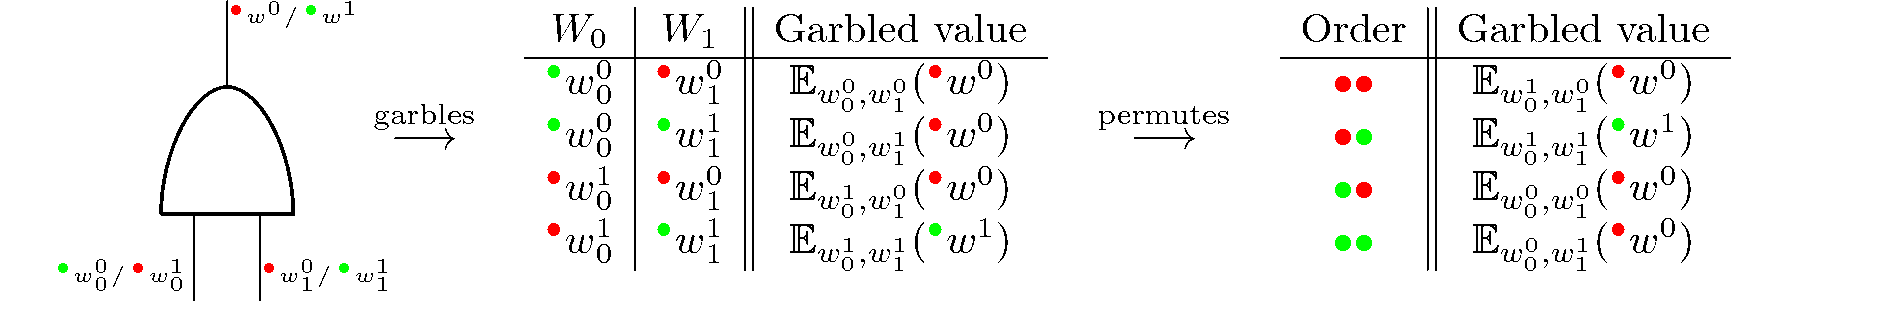
\includegraphics{./media/02.png}
\caption{AND garbled con permute on point}
\end{figure}

Queste modifiche permettono a Bob di decifrare semplicemente la voce il cui indice corrisponde ai colori associati ai suoi fili di ingresso e quindi di ottenere il valore del filo di uscita e il suo colore, permettendogli di valutare ulteriormente il circuito.

\hypertarget{esempio-di-valutazione}{%
\section{Esempio di Valutazione}\label{esempio-di-valutazione}}

\begin{figure}
\centering
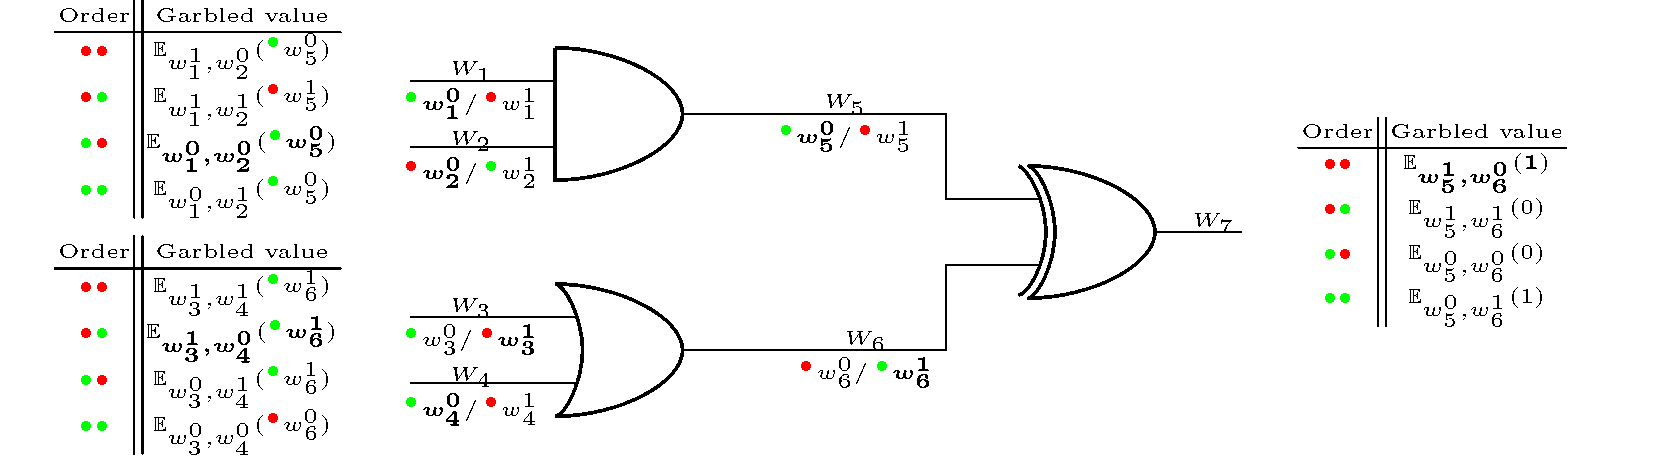
\includegraphics{./media/03.png}
\caption{AND garbled con permute on point}
\end{figure}

Vediamo ora come si potrebbe valutare il circuito confuso rappresentato nella Figura 2.3 usando il metodo permute-and-point che abbiamo discusso sopra. Assumiamo che i valori semantici di ingresso di \((W_1,W_2,W_3,W_4)\) siano \((0,0,1,0)\), il che significa che l'input confuso effettivo è \(({\color{green}\bullet}{}w_1^0,{\color{red}\bullet}{}w_2^0,{\color{red}\bullet}{}w_3^1,{\color{green}\bullet}{}w_4^0)\) dove gli \(w^i_j\) sono i valori casuali che Alice ha scelto quando ha confuso il circuito, come visto sopra. Assumiamo anche che Alice abbia già fornito il suo input confuso, diciamo \((W_1,W_3)\), e che Bob abbia già ottenuto il suo input confuso \((W_2,W_4)\) da Alice attraverso due applicazioni di Oblivious transfer come descritto nel paragrafo riguardante.

Bob comincerà quindi a valutare prima la porta AND utilizzando l'ingresso \(({\color{green}\bullet}{}w_1^0,{\color{red}\bullet}{}w_2^0)\), dato che ha i colori \(\color{green}\bullet\color{red}\bullet\) cercherà di decifrare la terza voce della GGT della porta AND, che funziona e quindi gli fornirà il valore confuso \({\color{green}\bullet}{}w_5^0\).

Potrà poi continuare la sua valutazione con la seconda porta, che è la porta OR. Guardando il suo ingresso \(({\color{red}\bullet}{}w_3^1,{\color{green}\bullet}{}w_4^0)\) e proverà a decifrare la voce corrispondente a \(\color{red}\bullet\color{green}\bullet\) con le chiavi \((w_3^1,w_4^0)\), essa si decifra nel valore confuso \({\color{green}\bullet}{}w_6^1\).

Potrà ora decifrare la porta XOR finale usando l'ingresso calcolato \(({\color{green}\bullet}{}w_5^0,{\color{green}\bullet}{}w_6^1)\), decifrando così la voce \(\color{green}\bullet\color{green}\bullet\) che gli fornisce il risultato finale: \(1\).

Bob non sa quale sia stato l'input di Alice, ne conosce solo l'output finale ``1'' e le stringhe generate casualmente \(w_1^0,w_2^0,w_3^1,w_4^0,w_5^0,w_6^1\). Egli può ancora, per esempio, dedurre dal circuito che i valori semantici di \(w_5^0\) e \(w_6^1\) sono opposti, tuttavia questo sistema non gli permette di invertire il circuito confuso fino ai valori di ingresso di Alice.

Ci sono circuiti in cui non è assicurata la privacy, come per esempio un circuito che calcola la somma degli ingressi. Tuttavia, in questo caso di esempio Bob, conoscendo i suoi valori semantici di ingresso, può semplicemente limitare gli ingressi di Alice a un sottoinsieme dei possibili ingressi, ma non può determinare in modo univoco i reali valori di ingresso di Alice.

\hypertarget{la-sintesi-dei-circuiti}{%
\chapter{La sintesi dei circuiti}\label{la-sintesi-dei-circuiti}}

Nel capitolo precedente abbiamo discusso dell'importanza della presenza di un circuito logico all'interno del protocollo creato da Yao. La scelta di un circuito efficiente rende la computazione e i tempi di calcolo delle operazioni non elevati. Ciò che rende efficace la scelta è trovare il giusto bilanciamento tra numero di input che le 2 parti coinvolte devono immettere nel circuito e, nel caso di un dominio multivalore, scegliere un dominio non troppo elevato che andrebbe ad immettere, per ogni valore di input, troppi valori che porterebbero ad aumentare i costi totali del circuito.

La scelta di questi circuiti viene facilitata dall'utilizzo di strumenti chiamati \emph{sintetizzatori}, questi tool sono stati creati per andare a ridurre le dimensioni dei circuiti dati loro in ingresso. All'interno di questo lavoro sono stati utilizzati 2 tool differenti: \textbf{MVSIS} e \textbf{ABC}, entrambi sono stati sviluppati nel tempo dall'università di Berkley, essi contengono diversi metodi di sintesi capaci di andare a eliminare nodi e ridondanze superflue nei circuiti e sintetizzare il circuito andandone a cambiare radicalmente la struttura interna de i nodi.

\newpage

\hypertarget{mvsis}{%
\section{MVSIS}\label{mvsis}}

MVSIS è il primo tool in grado di manipolare circuiti con una logica multivalore. Per la sua creazione si è preso come modello \textbf{SIS}, un tool sviluppato e specifico per la logica binaria, cercando di mantenerne simile la logica di funzionamento.

\hypertarget{design-specification}{%
\subsection{Design specification}\label{design-specification}}

Un circuito multivalore (MV circuit) può essere dato come valore di input a \textbf{MVSIS} tramite l'apposito comando (\texttt{read\_blifmv}), oltre a circuiti multivalore possono essere dati in input anche circuiti binari. Internamente, la rappresentazione del progetto è una rete di nodi MV; ogni nodo rappresenta una rappresenta una funzione MV con una singola uscita a più valori. Un'importante distinzione con alcuni altri metodi multivalore è che ogni variabile del nodo può avere un dominio diverso. L'intervallo per la variabile \(y_k\) è rappresentato dall'insieme \$P\_k=\{0,1,\ldots,p\_k -1 \}. La funzione il cui esito dà UN SET dei mintermi (Una sola uscita con 0 o 1) per i quali \(f_k = i\) (la funzione al nodo \(k\) è uguale al valore \(i\) ) è chiamata \emph{i-set} della funzione \(f_k\) e viene memorizzata in forma SOP (Somma di prodotti). Nel caso di logica a 2 valori, l'insieme 0 corrisponde all'off-set e l'insieme 1 all'on set. Una variabile MV yk è associata all'uscita del nodo k. Un margine congiunge \(k\) a \(j\) se uno qualsiasi degli i-set di \(j\) dipende esplicitamente da \(y_k\). La rete ha un insieme di ingressi primari (che possono essere tutti a più valori) e un insieme di nodi di ingressi primari.

\hypertarget{semplificazione-dei-nodi}{%
\subsection{Semplificazione dei nodi}\label{semplificazione-dei-nodi}}

L'i-set (uno per ogni valore di output) di un nodo multivalore può essere semplificato con 2 comandi:

\begin{itemize}
\tightlist
\item
  SIMPLIFY
\item
  FULLSIMP
\end{itemize}

FULLSIMP tra le 2 opzioni è quella che garantisce una semplificazione più efficace.Utilizza il CODC (Compatible Observability Don't Cares) e MV-image computation. Ogni i-set del nodo è poi semplificato da ESPRESSO-MV utilizzando i valori ricavati dalle 2 tecniche precedenti.

\newpage

\hypertarget{kernel-e-cube-extraction}{%
\subsection{Kernel e Cube Extraction}\label{kernel-e-cube-extraction}}

Un altro importante step nell'ottimizzazione del circuito consiste nell'applicare metodi algebrici per estrarre nuovi nodi che hanno divisori comuni per altri nodi. Si sono sviluppate nuove tecniche algebriche per la logica MV che trattano uniformemente le variabili binarie e multi-valore. Esse includono metodi per
trovare sottoespressioni comuni, divisione semi-algebrica, decomposizione di una rete multi-valore e fattorizzazione di una forma SOP. I comandi rilevanti e le brevi descrizioni delle loro capacità sono elencati di seguito.

\begin{enumerate}
\def\labelenumi{\arabic{enumi}.}
\tightlist
\item
  \textbf{FX}: estrae buoni divisori comuni e crea nuovi nodi nella rete, reimpostando altri nodi in termini di questi.
\item
  \textbf{Decomp}: fa una completa fattorizzazione multivaloriale degli i-sets di ogni nodo e suddivide i nodi secondo queste fattorizzazioni. Dopo questo, \textbf{resub}, usando la divisione algebrica multivalore, può essere eseguita per eliminare i fattori duplicati.
\end{enumerate}

\hypertarget{altri-comandi-per-la-manipolazione-dei-nodi}{%
\subsection{Altri comandi per la manipolazione dei nodi}\label{altri-comandi-per-la-manipolazione-dei-nodi}}

\begin{enumerate}
\def\labelenumi{\arabic{enumi}.}
\tightlist
\item
  \textbf{Collapsing}: converte l'intera rete multilivello in modo che le forme SOP per ogni uscita siano in termini di soli ingressi primari. Così il numero di nodi nella rete sarà esattamente il numero di uscite primarie.
\item
  \textbf{Merging}: Prende tutti i nodi e forza un'unione creando un singolo nodo multi-valore costruendo in \emph{i-set} per ogni combinazione di valori creata. Se ci sono più \emph{i-set} creati uguali vengono uniti in un singolo nodo.
\item
  \textbf{Encoding}: è come l'inverso del merging di funzioni binarie. Cerca di trovare una buona codifica binaria per ogni variabile multi-valore nella rete, compresi gli ingressi e le uscite primarie. Alla fine, ogni segnale è codificato come un segnale binario. Quindi un file binario può essere scritto. Formato da 2 fasi:

  \begin{enumerate}
  \def\labelenumii{\arabic{enumii}.}
  \tightlist
  \item
    Inizia dagli ingressi e per ogni nodo, determina se uno dei suoi fanin può essere usato per codificare parzialmente il nodo.
  \item
    inizia dalle uscite e in ordine topologico inverso lavora a ritroso fino agli ingressi primari. Ad ogni nodo, le sue uscite sono codificate utilizzando le informazioni su come sono utilizzati i suoi fanout
  \end{enumerate}
\item
  \textbf{Pair decoding}: Simile al merging ma utilizza un altro modo per scegliere quali modi unire.
\item
  \textbf{Bi-decomposition}: crea dei nodi multi-valore intermedi. Prende una rete MV appiattita o parzialmente appiattita e ne genera un'altra composta da porte MAX e MIN multi-valutate a due ingressi e da iterali multi-valutati. Vengono sfruttate sia l'incompletezza della specifica iniziale che le flessibilità generate nel processo di composizione.
\end{enumerate}

\hypertarget{abc}{%
\section{ABC}\label{abc}}

ABC è un sistema software in sviluppo per la sintesi e la verifica di circuiti logici sequenziali binari che appaiono in progetti hardware. ABC combina un'ottimizzazione logica scalabile basata su And-Inverter Graphs (AIGs), una mappatura tecnologica basata su DAG per tabelle di look-up e celle standard e algoritmi innovativi per la sintesi e la verifica sequenziale.

Questo programma nasce dalle esperienze assimilate dall'uso di SIS, VIS e MVSIS.
Questi sistemi non forniscono un ambiente di programmazione flessibile per implementare le recenti innovazioni. In particolare, l'ambiente SIS è obsoleto e piuttosto inefficiente nella gestione di grandi circuiti. VIS, progettato come strumento di verifica formale per specifiche multi-valore, non fornisce abbastanza flessibilità per la sintesi binaria. MVSIS nonostante il suo ampio utilizzo:

\begin{itemize}
\tightlist
\item
  Le strutture dati e gli algoritmi di base di MVSIS possono essere resi considerevolmente più semplici e facili da usare assumendo reti binarie,
\item
  Un posto centrale nel nuovo sistema dovrebbe essere dato a una nuova struttura dati, le AIG (reti logiche multilivello composte da AND e inverter a due ingressi), che promette miglioramenti nella qualità e nel tempo di esecuzione della sintesi e della verifica.
\end{itemize}

La comprensione di queste problematiche ha spinto a ri-sviluppare i pacchetti di base di MVSIS risultando in un nuovo ambiente di programmazione chiamato ABC. Come suggerisce il nome, l'obiettivo primario è quello di mantenere strutture di dati semplici e flessibili per una vasta gamma di applicazioni.

L'obiettivo del progetto ABC è quello di fornire un'implementazione pubblica degli algoritmi di sintesi combinatoria e sequenziale allo stato dell'arte e, allo stesso tempo, creare un ambiente open-source, in cui tali applicazioni possano essere sviluppate e confrontate. La versione attuale di ABC può ottimizzare/mappare/realizzare progetti industriali a livello di gate con 100K porte e 10K elementi sequenziali cont tempi di calcolo non superiori al minuto in un computer moderno.

\hypertarget{sintesi-combinatoria}{%
\subsection{Sintesi combinatoria}\label{sintesi-combinatoria}}

I metodi di logica combinatoria utilizzati da ABC all'interno dei suoi script (resyn e resyn2) sono tipicamente 10-100 volte più veloci se comparati agli script utilizzati all'interno di SIS o MVSIS.

In ABC, i confini dei nodi sono inizialmente distrutti dall'hashing strutturale (comando \emph{strash}), che trasforma una rete logica in un AIG. I confini possono essere ricreati su richiesta usando il comando \emph{renode}, che può essere visto come un inverso del comando SIS \emph{eliminate}. Nel flusso di sintesi presentato sopra la logica viene trasformata a livello di AIG senza creare nodi.

\begin{itemize}
\tightlist
\item
  \textbf{Balance}: prende come ingresso un AIG e lo bilancia.
\item
  \textbf{Cleanup}: Rimuove i nodi logici che non sono a ventaglio in PO e latches.
\item
  \textbf{Collapse}: Collassa tutto il circuito ad una rete ad un solo livello. Le funzioni dei nodi sono rappresentate utilizzando le BDD.
\item
  \textbf{Dsd}: Applica la decomposizione disjoint-support utilizzando l'algoritmo di Bertacco/Damiani \citep{ICCAD97}.
\item
  \textbf{fx}: Rileva la logica di condivisione estraendo i divisori a due cubi e i divisori a due lettere a un cubo usando l'algoritmo di Rajski/Vasudevamurthi \citep{TCAD92}.
\item
  \textbf{Multi}: Espande l'AIG a due ingressi in una rete di porte AND a più ingressi.
\item
  \textbf{refactor}: Esegue il collasso iterativo e il refactoring dei coni logici nell'AIG, che cerca di ridurre il numero di nodi AIG e il numero di livelli logici.
\item
  \textbf{renode}: Assume che l'input sia un AIG. Crea i confini dei nodi in questo AIG e collassa la logica intermedia per formare nodi più grandi.
\item
  \textbf{rewrite}: Assume che l'input sia un AIG. Crea i legami tra i nodi in questo AIG e collassa la logica intermedia per formare nodi più grandi.
\item
  \textbf{rr}: Esegue la rimozione della ridondanza per le AIG.
\item
  \textbf{strash}: Trasforma la rete corrente in un AIG tramite un livello di hashing strutturale. L'AIG risultante è una rete logica composta da porte AND a due ingressi e invertitori rappresentati come attributi complementari sui bordi. L'hashing strutturale è una trasformazione puramente combinatoria, che non modifica il numero e le posizioni delle porte.
\item
  \textbf{sweep}: sweep classico applicabile alla rete logica corrente che risulta in una rete logica. Sweep esegue i seguenti compiti: rimuove i nodi dangling (nodi senza fanout), collassa i buffer e gli inverter nei loro fanout, propaga le costanti, e rimuove i fanin duplicati. Sweep non può essere applicato a un AIG perché un AIG è strutturalmente hashed e quindi non ha buffer, invertitori e nodi costanti non propagati. Per rimuovere i nodi dandling nella rete logica, usate cleanup.
\end{itemize}

\newpage

\hypertarget{sintesi-sequenziale}{%
\subsection{Sintesi sequenziale}\label{sintesi-sequenziale}}

La sintesi sequenziale trasforma la rete corrente modificando la sua logica insieme agli elementi di memorizzazione (latches o flip-flops), se presenti. La rete risultante può avere una codifica di stato e uno spazio di stato diversi rispetto alla rete originale, ma le due reti sono sequenzialmente equivalenti (cioè, partendo dagli stati iniziali, per le stesse sequenze di vettori d'ingresso, producono sequenze identiche di vettori d'uscita).

\begin{itemize}
\tightlist
\item
  \textbf{Cycle}: Simula la rete sequenziale con un input casuale e aggiorna il suo stato attuale.
\item
  \textbf{init}: Ripristina gli stati iniziali di tutte le porte della rete corrente.
\item
  \textbf{lcorr} - Implementazione suddivisa di registro-corrispondenza usando l'induzione semplice. Rileva e fonde registri sequenzialmente equivalenti.
\item
  \textbf{retime}: Implementa diversi tipi di retiming:

  \begin{itemize}
  \tightlist
  \item
    most forward;
  \item
    most backward;
  \item
    minimum-register;
  \item
    minimum-delay euristico;
  \item
    delay-optimal retiming \citep{ICCD_1997}
  \end{itemize}

  Le porte sono condivise in modo ottimale attraverso gli archi di fanout quando il circuito è trasformato dall'AIG in una rete logica. Il calcolo degli stati iniziali dopo il retiming è ridotto a un problema SAT, che viene risolto usando MiniSat.
\item
  \textbf{scleanup}: Esegue la pulizia sequenziale (rimuove i nodi e le latches che non sono a fanout).
\item
  \textbf{ssw}: Implementa la segnali corrispondenti usando l'induzione K-step. Rileva e fonde i nodi sequenzialmente equivalenti.
\item
  \textbf{undc}: Si può utilizzare questo comando prima di eseguire la verifica sequenziale, per convertire i registri con gli stati iniziali don't-care in registri con uno stato iniziale costante-0.
\item
  \textbf{xsim}: Esegue la simulazione con valore \(X\) della rete sequenziale corrente.
\end{itemize}

\hypertarget{analisi}{%
\chapter{Analisi}\label{analisi}}

Il protocollo di Yao prevede, durante i suoi scambi, che le due parti concordino anche sulla trasmissione di un circuito a cui entrambi gli attori debbano inserire dei valori di input. Uno degli scopi della nostra tesi consiste nel testare l'efficacia dell'utilizzo di un multi valore rispetto all'utilizzo ``classico'' di un circuito booleano concentrandoci sul fattore di costo computazionale delle operazioni.

Siamo partiti quindi selezionando un set di circuiti binari con differente numero di ingressi, uscite e livelli. Con questa base ci si è poi concentrati sul trovare una metodologia di conversione dei circuiti per portarli da un `classico' dominio booleano ad uno multi-valore dove i valori non sono più rappresentati sa 0 e 1 ma da da un set più ampio di valori ma mantenendo le funzionalità del circuito. Una volta ottenuta una controparte per ogni circuito si è proceduto con un confronto dei circuiti in modo da individuare quali di questi set siano più efficaci.

\newpage

\hypertarget{studio-del-circuito-binario}{%
\section{Studio del circuito binario}\label{studio-del-circuito-binario}}

Analizzando i circuiti per testare la nostra tesi abbiamo dovuto sviluppare una tecnica di conversione dei circuiti binari di partenza. Le caratteristiche di una naturale rappresentazione di un circuito consiste nella sua divisione in nodi, ognuno di essi rappresentato da una tabella di verità i cui input e output vanno a collegarsi tra di loro tramite dei collegamenti. Soffermandoci sulle tabelle di verità abbiamo notato come andando ad applicare un raggruppamento di \(n\) bit per ogni riga della tabella si riuscirebbe a rappresentare un valore di dominio più grande di quello binario del circuito in analisi riducendo il numero di input richiesti dal gate.

\[\begin{matrix}
    \underbrace{10} & \underbrace{11} & \underbrace{00} \\
    \downarrow & \downarrow & \downarrow  &mod_3 \\
    2 & 3 & 0
\end{matrix}\]

Con questo approccio non andiamo a snaturare quella che è la logica della tabella originale poiché, sapendo il qual è il nuovo dominio applicato, riusciamo ad invertire il processo di conversione ritornando al circuito originale.

I vincoli di questo approccio di conversione dei circuiti booleani risiede nel fatto che, per ora, la conversione possa essere fatta solamente con un numero pari di input e che il numero di output sia un divisore del numero di bit utilizzati per il raggruppamento.

\newpage

Una volta definito il metodo di conversione si è passati alla scelta del nuovo dominio da applicare ai circuiti con l'obiettivo di trovare il giusto compromesso per ottenere:

\begin{itemize}
\item
  Una riduzione degli input che faccia diminuire il costo del circuito di ingresso per il circuito di ingresso
\item
  Utilizzare un dominio che risulti controproducente: avere un dominio superiore a quello booleano ma troppo elevato significherebbe che, per ogni input, ogni parte dovrebbe portare inserire tanti valori di input quanti quelli del dominio richiesto e, se si sceglie un dominio troppo grande, nonostante la riduzione degli input ci si troverebbe comunque con un costo totale del circuito elevato. Si è deciso quindi di sperimentare 2 approcci alla scelta di questo valore, uno statico e uno dinamico.

  \begin{itemize}
  \tightlist
  \item
    \textbf{Statico}: per ognuno dei circuiti andremo ad applicare lo stesso valore di dominio, il valore scelto è 3, andremo quindi a raggruppare ogni 2 valori per riga della tabella di verità;
  \item
    \textbf{Dinamico}: ogni circuito viene analizzato andando a trovare il numero di input e output, successivamente viene calcolato il valore di M.C.D. e:

    \begin{itemize}
    \tightlist
    \item
      Se il valore trovato consente alla tabella di verità convertita di avere almeno 2 valori di input si utilizza quel valore per raggruppare i bit delle righe, altrimenti il valore viene dimezzato
    \item
      Se il valore risultante è un numero che creerebbe un dominio troppo grande viene utilizzato il dominio 3, come nel caso statico.
    \end{itemize}
  \end{itemize}
\end{itemize}

Definite tutte le logiche di conversione si è dovuto cercare un formato di file che rappresentasse i circuiti che rispettasse le esigenze per applicare tutte le elaborazioni sopra descritte e che sia utilizzato come uno standard di rappresentazione in modo che i risultati ottenuti possano essere utilizzati dai software di sintesi che andremo ad utilizzare successivamente durante l'elaborazione della sperimentazione. Si necessita dunque di una rappresentazione che abbia la possibilità che i circuiti con output multipli siano rappresentati sulla stessa linea all'interno della tabella della verità.

Tra i vari formati a disposizione la scelta è ricaduta sul formato \texttt{PLA} già ampiamente utilizzato per la rappresentazione di circuiti.

\newpage

\hypertarget{analisi-della-struttura-pla}{%
\subsection{Analisi della struttura PLA}\label{analisi-della-struttura-pla}}

Un file PLA ha la seguente struttura

\begin{verbatim}
.i 4
.o 2
.ilb x1 x2 y1 y2
.ob f1 f2
0--0 00    
0001 01
0-11 --
1-11 01
0101 10
10-- 01
11-- 00
.end
\end{verbatim}

Questo \texttt{PLA} di esempio rappresenta un circuito composto da una sola tabella di verità, la sintassi va a descrivere:

\begin{itemize}
\tightlist
\item
  \texttt{.i}: numero di valori di input;
\item
  \texttt{.o}: numero di valori di output;
\item
  \texttt{.ilb}: nomi e ordine delle variabili di input;
\item
  \texttt{.ob}: nomi e ordine delle variabili di output.
\end{itemize}

Il resto del file rappresenta la tabella di verità con i possibile valori che si ottengono combinando i valori di input\_file per ottenere gli output.Il circuito sopra descritto presenta 4 variabili di input e 2 valori di output. Come possiamo notare all'interno della tabella di verità non tutti i valori sono booleani ma è presente anche il valore \texttt{-}, esso prende il nome di \textbf{don't care} e può assumere 2 significati:

\begin{itemize}
\tightlist
\item
  Quando \texttt{-} è presente negli output di una riga significa che l'output per quella determinata riga non mi interessa;
\item
  Quando \texttt{-} è presente negli input significa che in quella posizione la variabile a cui fa riferimento può assumere un qualsiasi valore non andando ad influire sul valore di output che si andrà ad ottenere.
\end{itemize}

\newpage

\hypertarget{la-gestione-dei-dont-care-durante-la-conversione}{%
\subsection{La gestione dei don't care durante la conversione}\label{la-gestione-dei-dont-care-durante-la-conversione}}

I dont't care sono una caratteristica dei file pla che deve essere gestita in modo funzionale ai cambi di dominio che andremo a fare all'interno delle tabelle di verità dei nostri circuiti in quanto, se affrontato nel modo sbagliato, modificherebbe la logica dell'intero circuito rendendo la conversione errata. Per spiegare meglio come tratteremo questa caratteristica dei \textbf{PLA} presenterò l'esempio di un esempio utilizzando un circuito semplice che come valore di dominio di conversione il valore 3. Il circuito avrà la seguente struttura.

\begin{verbatim}
.i 4
.o 2
.ilb x1 x2 y1 y2
.ob f1 f2
0--0 00    
0001 01
0-11 --
1-11 01
0101 10
10-- 01
11-- 00
.end
\end{verbatim}

Una volta deciso il nostro nuovo dominio di conversione sappiamo di quanti bit dobbiamo raggruppare per rappresentare il nostro nuovo dominio, nel nostro caso essendo il domino 3, il numero di bit per rappresentare il valore più grande di questo dominio abbiamo bisogno di un raggruppamento a 2 bit. Procediamo quindi a scandire riga per riga il circuito raggruppando i bit a blocchi di 2 tutti i valori di input e di output.

\begin{verbatim}
0- -0 00    
00 01 01
0- 11 --
1- 11 01
01 01 10
10 -- 01
11 -- 00
\end{verbatim}

Una volta creati questi cluster di bit ci accorgiamo come i dont't care in alcuni casi ci rendano impossibile la conversione al nuovo dominio, per risolvere questo problema dovremo andare a sviluppare questi valori di don't care in `normali' valori booleani.

\newpage

Non è sempre necessario andare a sviluppare i don't care, andiamo a differenziare 2 possibili casistiche di intervento:

\begin{itemize}
\tightlist
\item
  Quando il numero di `-' è uguale al numero di bit del raggruppamento multivalore, in questo caso non c'è la necessità di sviluppare i valori, sarà sufficiente inserire al posto della coppia un unovo \texttt{-} rappresentante il don't care.
  \[ \begin{array}{ccc}
        10 & -- & 01 \\ & \downarrow & \\ 2 & - & 1 
    \end{array}\]
\item
  Quando nel gruppo di bit raggruppati il numero di \texttt{-} è minore del numero di bit richiesti. In questo caso dobbiamo procedere con l'espansione del dont't care a valori di verità in modo da poter affrontare correttamente la conversione nel nuovo dominio.
  \[ \begin{array}{cccc}
            1- & 11 & 01\\
            & \downarrow &\\
            10 & 11 & 01\\
            11 & 11 & 01\\
            & \downarrow &\\
            2 & 3 & 1\\
            3 & 3 & 1
        \end{array}\]
\end{itemize}

\newpage

Così facendo è possibile sviluppare tutto il circuito binario e ottenere una conversione esatta. Il circuito convertito
sarà quindi.

\begin{verbatim}
00 0
02 0
10 0
12 0
01 1
03 -
13 -
23 1
11 2
2- 1
3- 0
\end{verbatim}

Con questa struttura è dunque possibile procedere con l'analisi dei circuiti proseguendo con l'attività di sintesi logica.

\hypertarget{implementazione-della-conversione}{%
\section{Implementazione della conversione}\label{implementazione-della-conversione}}

La conversione dei circuiti in analisi viene implementata utilizzando il linguaggio di programmazione Python nella versione 3.8 senza l'ausilio di nessun package esterno, vengono utilizzate solamente librerie comprese nel linguaggio. Questa dinamica fa si che il sistema sia ``ready to use'' una volta installato il linguaggio di programmazione se non già presente all'interno del SO.

\hypertarget{analisi-del-circuito}{%
\subsection{Analisi del circuito}\label{analisi-del-circuito}}

\begin{Shaded}
\begin{Highlighting}[]
\KeywordTok{def}\NormalTok{ read\_pla(path\_file):}
\NormalTok{    inp }\OperatorTok{=} \VariableTok{None}
\NormalTok{    out }\OperatorTok{=} \VariableTok{None}
\NormalTok{    inp\_array }\OperatorTok{=}\NormalTok{ []}
\NormalTok{    out\_array }\OperatorTok{=}\NormalTok{ []}
\NormalTok{    truth\_table }\OperatorTok{=}\NormalTok{ []}
    \ControlFlowTok{with} \BuiltInTok{open}\NormalTok{(path\_file, }\StringTok{\textquotesingle{}r\textquotesingle{}}\NormalTok{) }\ImportTok{as}\NormalTok{ input\_file:}
        \ControlFlowTok{for}\NormalTok{ line }\KeywordTok{in}\NormalTok{ input\_file.readlines():}
            \ControlFlowTok{if} \StringTok{\textquotesingle{}.i\textquotesingle{}} \KeywordTok{in}\NormalTok{ line }\KeywordTok{and}\NormalTok{ line[}\DecValTok{2}\NormalTok{] }\OperatorTok{==} \StringTok{\textquotesingle{} \textquotesingle{}}\NormalTok{:}
\NormalTok{                inp }\OperatorTok{=}\NormalTok{ line.split(}\StringTok{\textquotesingle{} \textquotesingle{}}\NormalTok{)[}\DecValTok{1}\NormalTok{]}
            \ControlFlowTok{elif} \StringTok{\textquotesingle{}.o\textquotesingle{}} \KeywordTok{in}\NormalTok{ line }\KeywordTok{and}\NormalTok{ line[}\DecValTok{2}\NormalTok{] }\OperatorTok{==} \StringTok{\textquotesingle{} \textquotesingle{}}\NormalTok{:}
\NormalTok{                out }\OperatorTok{=}\NormalTok{ line.split(}\StringTok{\textquotesingle{} \textquotesingle{}}\NormalTok{)[}\DecValTok{1}\NormalTok{]}
            \ControlFlowTok{elif} \StringTok{\textquotesingle{}.ilb\textquotesingle{}} \KeywordTok{in}\NormalTok{ line:}
\NormalTok{                inp\_array }\OperatorTok{=}\NormalTok{ line.strip().split(}\StringTok{\textquotesingle{} \textquotesingle{}}\NormalTok{)[}\DecValTok{1}\NormalTok{:]}
            \ControlFlowTok{elif} \StringTok{\textquotesingle{}.ob\textquotesingle{}} \KeywordTok{in}\NormalTok{ line:}
\NormalTok{                out\_array }\OperatorTok{=}\NormalTok{ line.strip().split(}\StringTok{\textquotesingle{} \textquotesingle{}}\NormalTok{)[}\DecValTok{1}\NormalTok{:]}
            \ControlFlowTok{elif} \StringTok{\textquotesingle{}.end\textquotesingle{}} \KeywordTok{in}\NormalTok{ line:}
                \ControlFlowTok{continue}
            \ControlFlowTok{else}\NormalTok{:}
\NormalTok{                line }\OperatorTok{=}\NormalTok{ \{}
                    \StringTok{\textquotesingle{}inp\textquotesingle{}}\NormalTok{:  line.strip().split(}\StringTok{\textquotesingle{} \textquotesingle{}}\NormalTok{)[}\DecValTok{0}\NormalTok{],}
                    \StringTok{\textquotesingle{}out\textquotesingle{}}\NormalTok{:  line.strip().split(}\StringTok{\textquotesingle{} \textquotesingle{}}\NormalTok{)[}\DecValTok{1}\NormalTok{]}
\NormalTok{                \}}
\NormalTok{                truth\_table.append(line)}
    \ControlFlowTok{return}\NormalTok{ inp, out, inp\_array, out\_array, truth\_table}
\end{Highlighting}
\end{Shaded}

La funzione prende in input un circuito binario in formato PLA e, riga per riga, analizza le informazioni in base al prefisso all'interno di ogni riga del file che va a differenziare le informazioni del circuito. Scandendo il fil recupera:

\begin{itemize}
\tightlist
\item
  Tabella delle verità
\item
  Numero di input
\item
  Numero di output
\item
  Array contenente il nome delle variabili di input;
\item
  Array contenente il nome delle variabili di output;
\end{itemize}

Queste informazioni serviranno successivamente per convertire il circuito e calcolare costi.

\hypertarget{espansione-dei-dont-care}{%
\subsection{Espansione dei don't care}\label{espansione-dei-dont-care}}

Una volta ottenuto tutte le informazioni disponibili dal circuito dato bisogna andare ad identificare all'interno delle tabelle di verità quali sono i \emph{don't care} a cui bisogna espandere i valori e quelli che si possono ignorare. Questo passaggio è stato la parte più impegnativa riguardante le funzionalità del programma.

\begin{Shaded}
\begin{Highlighting}[]
\NormalTok{n\_dont\_care }\OperatorTok{=} \StringTok{\textquotesingle{}\textquotesingle{}}
    \ControlFlowTok{for}\NormalTok{ i }\KeywordTok{in} \BuiltInTok{range}\NormalTok{(dv):}
\NormalTok{        n\_dont\_care }\OperatorTok{+=} \StringTok{\textquotesingle{}{-}\textquotesingle{}}
\end{Highlighting}
\end{Shaded}

\newpage

Questo semplice ciclo va a replicare il numero di \texttt{-} consecutivi che rispecchiano i gruppi di don't care da ignorare in base al dominio di conversione dato al circuito.

\begin{Shaded}
\begin{Highlighting}[]
\NormalTok{len\_truth\_table }\OperatorTok{=} \BuiltInTok{len}\NormalTok{(truth\_table)}
\NormalTok{i }\OperatorTok{=} \DecValTok{0}
\ControlFlowTok{while}\NormalTok{ i }\OperatorTok{\textless{}}\NormalTok{ len\_truth\_table:}
    \ControlFlowTok{if} \StringTok{\textquotesingle{}{-}\textquotesingle{}} \KeywordTok{in}\NormalTok{ truth\_table[i][}\StringTok{\textquotesingle{}inp\textquotesingle{}}\NormalTok{]:}
\NormalTok{        truth\_table[i][}\StringTok{\textquotesingle{}inp\textquotesingle{}}\NormalTok{] }\OperatorTok{=} \StringTok{\textquotesingle{}\textquotesingle{}}\NormalTok{.join(truth\_table[i[}\StringTok{\textquotesingle{}inp\textquotesingle{}}\NormalTok{])}
\NormalTok{        truth\_table[i][}\StringTok{\textquotesingle{}inp\textquotesingle{}}\NormalTok{] }\OperatorTok{=}\NormalTok{ [truth\_table[i][}\StringTok{\textquotesingle{}inp\textquotesingle{}}\NormalTok{[a:a}\OperatorTok{+}\NormalTok{dv]}
                                 \ControlFlowTok{for}\NormalTok{ a }\KeywordTok{in} \BuiltInTok{range}\NormalTok{(}\DecValTok{0}\NormalTok{, le(truth\_table[i][}\StringTok{\textquotesingle{}inp\textquotesingle{}}\NormalTok{], dv)]}
        \ControlFlowTok{for}\NormalTok{ a }\KeywordTok{in} \BuiltInTok{range}\NormalTok{(}\BuiltInTok{len}\NormalTok{(truth\_table[i][}\StringTok{\textquotesingle{}inp\textquotesingle{}}\NormalTok{])):}
            \ControlFlowTok{if}\NormalTok{ truth\_table[i][}\StringTok{\textquotesingle{}inp\textquotesingle{}}\NormalTok{][a] }\OperatorTok{==}\NormalTok{ n\_dont\_care:}
\NormalTok{                truth\_table[i][}\StringTok{\textquotesingle{}inp\textquotesingle{}}\NormalTok{][a] }\OperatorTok{=} \StringTok{\textquotesingle{}k\textquotesingle{}}\OperatorTok{*}\NormalTok{le(n\_dont\_care)}
\NormalTok{        truth\_table[i][}\StringTok{\textquotesingle{}inp\textquotesingle{}}\NormalTok{] }\OperatorTok{=} \StringTok{\textquotesingle{}\textquotesingle{}}\NormalTok{.join(truth\_table[i[}\StringTok{\textquotesingle{}inp\textquotesingle{}}\NormalTok{])}
\NormalTok{        new\_lines }\OperatorTok{=}\NormalTok{ resolve\_dont\_care(truth\_table[i],}\StringTok{\textquotesingle{}inp\textquotesingle{}}\NormalTok{)}
\NormalTok{        truth\_table }\OperatorTok{=}\NormalTok{ truth\_table[:i] }\OperatorTok{+}\NormalTok{ new\_lines }\OperatorTok{+}\NormalTok{truth\_table[i}\OperatorTok{+}\DecValTok{1}\NormalTok{:]}
\NormalTok{        len\_truth\_table }\OperatorTok{=} \BuiltInTok{len}\NormalTok{(truth\_table)}
\NormalTok{    i }\OperatorTok{+=} \DecValTok{1}
\end{Highlighting}
\end{Shaded}

Per andare a differenziare quali siano i \emph{don't care} da espandere e quali no a quest ultimi viene sostituito il simbolo \emph{-} con un valore \emph{k} in modo da poterli gestire meglio nelle funzioni successive. Alla fine delle operazioni verranno ripristinati con il simbolo corretto.

\newpage

\hypertarget{resolve-dont-care}{%
\subsubsection{Resolve don't care}\label{resolve-dont-care}}

\begin{Shaded}
\begin{Highlighting}[]
\KeywordTok{def}\NormalTok{ resolve\_dont\_care(line, in\_out):}
    \CommentTok{\# Conto qunati {-} e creo 2\^{}n nuove linee}
\NormalTok{    n\_dc }\OperatorTok{=} \BuiltInTok{pow}\NormalTok{(}\DecValTok{2}\NormalTok{, line[in\_out].count(}\StringTok{\textquotesingle{}{-}\textquotesingle{}}\NormalTok{))}

\NormalTok{    input\_entry }\OperatorTok{=}\NormalTok{ line[in\_out]}
\NormalTok{    new\_array }\OperatorTok{=}\NormalTok{ []}

    \ControlFlowTok{for}\NormalTok{ h }\KeywordTok{in} \BuiltInTok{range}\NormalTok{(line[in\_out].count(}\StringTok{\textquotesingle{}{-}\textquotesingle{}}\NormalTok{)):}
\NormalTok{        val\_array }\OperatorTok{=}\NormalTok{ create\_0\_1\_array(n\_dc, }\BuiltInTok{pow}\NormalTok{(}\DecValTok{2}\NormalTok{, h))}
        \ControlFlowTok{if}\NormalTok{ h }\OperatorTok{==} \DecValTok{0}\NormalTok{:}
            \ControlFlowTok{for}\NormalTok{ i }\KeywordTok{in} \BuiltInTok{range}\NormalTok{(n\_dc):}
\NormalTok{                it }\OperatorTok{=} \DecValTok{0}
\NormalTok{                new\_line }\OperatorTok{=}\NormalTok{ []}
                \ControlFlowTok{for}\NormalTok{ j }\KeywordTok{in} \BuiltInTok{range}\NormalTok{(}\BuiltInTok{len}\NormalTok{(input\_entry)}\OperatorTok{{-}}\DecValTok{1}\NormalTok{, }\OperatorTok{{-}}\DecValTok{1}\NormalTok{, }\OperatorTok{{-}}\DecValTok{1}\NormalTok{):}
                    \ControlFlowTok{if}\NormalTok{ input\_entry[j] }\OperatorTok{==} \StringTok{\textquotesingle{}{-}\textquotesingle{}} \KeywordTok{and}\NormalTok{ it }\OperatorTok{==} \DecValTok{0}\NormalTok{:}
\NormalTok{                        new\_line.append(val\_array[(}\BuiltInTok{len}\NormalTok{(val\_array)}\OperatorTok{{-}}\DecValTok{1}\NormalTok{) }\OperatorTok{{-}}\NormalTok{ i])}
\NormalTok{                        it }\OperatorTok{+=} \DecValTok{1}
                    \ControlFlowTok{else}\NormalTok{:}
\NormalTok{                        new\_line.append(line[in\_out][j])}
\NormalTok{                new\_array.append(new\_line[::}\OperatorTok{{-}}\DecValTok{1}\NormalTok{])}
        \ControlFlowTok{else}\NormalTok{:}
\NormalTok{            it }\OperatorTok{=} \DecValTok{0}
            \ControlFlowTok{for}\NormalTok{ c, l }\KeywordTok{in} \BuiltInTok{enumerate}\NormalTok{(new\_array):}
                \ControlFlowTok{for}\NormalTok{ j }\KeywordTok{in} \BuiltInTok{range}\NormalTok{(}\BuiltInTok{len}\NormalTok{(l)}\OperatorTok{{-}}\DecValTok{1}\NormalTok{, }\OperatorTok{{-}}\DecValTok{1}\NormalTok{, }\OperatorTok{{-}}\DecValTok{1}\NormalTok{):}
                    \ControlFlowTok{if}\NormalTok{ l[j] }\OperatorTok{==} \StringTok{\textquotesingle{}{-}\textquotesingle{}} \KeywordTok{and}\NormalTok{ it }\OperatorTok{==} \DecValTok{0}\NormalTok{:}
\NormalTok{                        l[j] }\OperatorTok{=}\NormalTok{ val\_array[(}\BuiltInTok{len}\NormalTok{(val\_array)}\OperatorTok{{-}}\DecValTok{1}\NormalTok{) }\OperatorTok{{-}}\NormalTok{ c]}
\NormalTok{                        it }\OperatorTok{+=} \DecValTok{1}
\NormalTok{                it }\OperatorTok{=} \DecValTok{0}

    \ControlFlowTok{if}\NormalTok{ in\_out }\OperatorTok{==} \StringTok{\textquotesingle{}inp\textquotesingle{}}\NormalTok{:}
        \ControlFlowTok{return}\NormalTok{ [\{}\StringTok{\textquotesingle{}inp\textquotesingle{}}\NormalTok{:  l, }\StringTok{\textquotesingle{}out\textquotesingle{}}\NormalTok{:  line[}\StringTok{\textquotesingle{}out\textquotesingle{}}\NormalTok{]\} }\ControlFlowTok{for}\NormalTok{ l }\KeywordTok{in}\NormalTok{ new\_array]}
    \ControlFlowTok{else}\NormalTok{:}
        \ControlFlowTok{return}\NormalTok{ [\{}\StringTok{\textquotesingle{}inp\textquotesingle{}}\NormalTok{:  line[}\StringTok{\textquotesingle{}inp\textquotesingle{}}\NormalTok{], }\StringTok{\textquotesingle{}out\textquotesingle{}}\NormalTok{:  l\} }\ControlFlowTok{for}\NormalTok{ l }\KeywordTok{in}\NormalTok{ new\_array]}
\end{Highlighting}
\end{Shaded}

Questa funzione prende in ingresso la linea da espandere e per ogni sua iterazione \emph{(it)} va a sostituire ogni simbolo \texttt{-} con un valore di verità. La funzione restituirà la l'espansione della linea.

\newpage

Come possiamo notare dal \texttt{return} della funzione questa operazione di espansione è possibile sia sugli input che su gli output.

\hypertarget{create_0_1_array}\NormalTok{ (count\_1 }\OperatorTok{+}\NormalTok{ count\_0) }\OperatorTok{\textless{}}\NormalTok{ count\_1 }
        \ControlFlowTok{else} \BuiltInTok{str}\NormalTok{(}\DecValTok{0}\NormalTok{) }\ControlFlowTok{for}\NormalTok{ i }\KeywordTok{in} \BuiltInTok{range}\NormalTok{(le)]}
\end{Highlighting}
\end{Shaded}

Questa funzione restituisce una tabella di verità data una line con all'interno un numero di \emph{don't care} che necessitano di espansione.

Questo tabella creata verrà inserita al posto della linea con i \emph{don't care} del circuito in così da avere la tabella corretta per la conversione.

\newpage

\hypertarget{la-conversione-in-multi-valore}{%
\section{La conversione in multi valore}\label{la-conversione-in-multi-valore}}

Le funzioni viste nelle sezioni precedenti restituiscono come valore di output una matrice corrispondente alla tabella della verità sviluppata. Questa tabella verrà utilizzata dalla funzione di conversione seguendo lo schema spiegato all'inizio del capitolo.

\begin{Shaded}
\begin{Highlighting}[]
\KeywordTok{def}\NormalTok{ create\_mv\_truth\_table(truth\_array, dv):}
\NormalTok{    conv\_truth }\OperatorTok{=}\NormalTok{ []}
    \ControlFlowTok{for}\NormalTok{ line }\KeywordTok{in}\NormalTok{ truth\_array:}
\NormalTok{        line[}\StringTok{\textquotesingle{}inp\textquotesingle{}}\NormalTok{] }\OperatorTok{=} \StringTok{\textquotesingle{}\textquotesingle{}}\NormalTok{.join(line[}\StringTok{\textquotesingle{}inp\textquotesingle{}}\NormalTok{])}
\NormalTok{        line[}\StringTok{\textquotesingle{}inp\textquotesingle{}}\NormalTok{] }\OperatorTok{=}\NormalTok{ [line[}\StringTok{\textquotesingle{}inp\textquotesingle{}}\NormalTok{][i }\OperatorTok{*}\NormalTok{ dv:(i }\OperatorTok{+} \DecValTok{1}\NormalTok{) }\OperatorTok{*}\NormalTok{ dv]}
            \ControlFlowTok{for}\NormalTok{ i }\KeywordTok{in} \BuiltInTok{range}\NormalTok{((}\BuiltInTok{len}\NormalTok{(line[}\StringTok{\textquotesingle{}inp\textquotesingle{}}\NormalTok{]) }\OperatorTok{+}\NormalTok{ dv }\OperatorTok{{-}} \DecValTok{1}\NormalTok{) }\OperatorTok{//}\NormalTok{ dv)]}
        \ControlFlowTok{if} \StringTok{\textquotesingle{}{-}\textquotesingle{}} \KeywordTok{not} \KeywordTok{in}\NormalTok{ line[}\StringTok{\textquotesingle{}out\textquotesingle{}}\NormalTok{]:}
\NormalTok{            line[}\StringTok{\textquotesingle{}out\textquotesingle{}}\NormalTok{] }\OperatorTok{=} \StringTok{\textquotesingle{}\textquotesingle{}}\NormalTok{.join(line[}\StringTok{\textquotesingle{}out\textquotesingle{}}\NormalTok{])}
\NormalTok{            line[}\StringTok{\textquotesingle{}out\textquotesingle{}}\NormalTok{] }\OperatorTok{=}\NormalTok{ [line[}\StringTok{\textquotesingle{}out\textquotesingle{}}\NormalTok{][i }\OperatorTok{*}\NormalTok{ dv:(i }\OperatorTok{+} \DecValTok{1}\NormalTok{) }\OperatorTok{*}\NormalTok{ dv]}
                \ControlFlowTok{for}\NormalTok{ i }\KeywordTok{in} \BuiltInTok{range}\NormalTok{((}\BuiltInTok{len}\NormalTok{(line[}\StringTok{\textquotesingle{}out\textquotesingle{}}\NormalTok{]) }\OperatorTok{+}\NormalTok{ dv }\OperatorTok{{-}} \DecValTok{1}\NormalTok{) }\OperatorTok{//}\NormalTok{ dv)]}
\NormalTok{            l\_supp\_inp }\OperatorTok{=}\NormalTok{ []}
\NormalTok{            l\_supp\_out }\OperatorTok{=}\NormalTok{ []}
            \ControlFlowTok{for}\NormalTok{ val }\KeywordTok{in}\NormalTok{ line[}\StringTok{\textquotesingle{}inp\textquotesingle{}}\NormalTok{]:}
                \ControlFlowTok{if} \StringTok{\textquotesingle{}{-}\textquotesingle{}} \KeywordTok{not} \KeywordTok{in}\NormalTok{ val:}
\NormalTok{                    l\_supp\_inp.append(}\BuiltInTok{int}\NormalTok{(val, }\DecValTok{2}\NormalTok{))}
                \ControlFlowTok{else}\NormalTok{:}
\NormalTok{                    l\_supp\_inp.append(}\StringTok{\textquotesingle{}{-}\textquotesingle{}}\NormalTok{)}
            \ControlFlowTok{for}\NormalTok{ val }\KeywordTok{in}\NormalTok{ line[}\StringTok{\textquotesingle{}out\textquotesingle{}}\NormalTok{]:}
\NormalTok{                l\_supp\_out.append(}\BuiltInTok{int}\NormalTok{(val, }\DecValTok{2}\NormalTok{))}
\NormalTok{            conv\_truth.append(\{}
                \StringTok{\textquotesingle{}inp\textquotesingle{}}\NormalTok{:  l\_supp\_inp,}
                \StringTok{\textquotesingle{}out\textquotesingle{}}\NormalTok{:  l\_supp\_out}
\NormalTok{            \})}
    \ControlFlowTok{return}\NormalTok{ conv\_truth}
\end{Highlighting}
\end{Shaded}

La funzione prende in ingresso la matrice espansa creata precedentemente e il numero di bit da utilizzare per rappresentare il massimo numero del nuovo dominio multivalore.

Inizialmente la funzione `spezza' la stringa dei valori di input in gruppi di tanti elementi quanti sono i bit per rappresentare il massimo numero, successivamente viene controllato se il gruppo è composto da:

\begin{itemize}
\tightlist
\item
  \textbf{dont't care}: si procede sostituendo con un singolo simbolo `-'
\item
  \textbf{numeri binari}: si procede con la conversione tramite il metodo int(), ad esso servono 2 parametri:

  \begin{itemize}
  \tightlist
  \item
    un numero o una stringa di numeri da convertire
  \item
    la base a cui si vuole fare la conversione
  \end{itemize}
\end{itemize}

Una volta scandita tutta la tabella di verità siamo giunti al circuito convertito, l'utlimo passo ora consiste nell'andare a creare un file compatibile per la sintesi dei circuiti.

\hypertarget{la-creazione-del-file-blfmv}{%
\section{La creazione del file blfmv}\label{la-creazione-del-file-blfmv}}

Per i circuiti multi valore non viene adottato il formato PLA in quanto viene utilizzato solamente per i circuiti binari. Facciamo uso di un altro formato standard appositamente creato per la logica multi valore, il formato \emph{blfmv}.

Questo formato deriva dal formato \emph{blif} utilizzato per la logica binaria.

\begin{Shaded}
\begin{Highlighting}[]
\ImportTok{import}\NormalTok{ string}
\NormalTok{mv\_input }\OperatorTok{=}\NormalTok{ [i }\ControlFlowTok{for}\NormalTok{ i }\KeywordTok{in} \BuiltInTok{list}\NormalTok{(string.ascii\_lowercase)[}
\NormalTok{    :}\BuiltInTok{len}\NormalTok{(mv\_table[}\DecValTok{0}\NormalTok{][}\StringTok{\textquotesingle{}inp\textquotesingle{}}\NormalTok{])]]}
\NormalTok{mv\_output }\OperatorTok{=}\NormalTok{ [}\StringTok{\textquotesingle{}o}\SpecialCharTok{\{\}}\StringTok{\textquotesingle{}}\NormalTok{.}\BuiltInTok{format}\NormalTok{(i) }\ControlFlowTok{for}\NormalTok{ i }\KeywordTok{in} \BuiltInTok{range}\NormalTok{(}\BuiltInTok{len}\NormalTok{(mv\_table[}\DecValTok{0}\NormalTok{][}\StringTok{\textquotesingle{}out\textquotesingle{}}\NormalTok{]))]}
\ControlFlowTok{with} \BuiltInTok{open}\NormalTok{(}\StringTok{\textquotesingle{}}\SpecialCharTok{\{\}}\StringTok{/blfmv/}\SpecialCharTok{\{\}}\StringTok{.mv\textquotesingle{}}\NormalTok{.}\BuiltInTok{format}\NormalTok{(working\_dir, nomefile), }\StringTok{\textquotesingle{}w\textquotesingle{}}\NormalTok{) }\ImportTok{as}\NormalTok{ blif:}
\NormalTok{    blif.write(}\StringTok{\textquotesingle{}.model }\SpecialCharTok{\{\}}\CharTok{\textbackslash{}n}\StringTok{\textquotesingle{}}\NormalTok{.}\BuiltInTok{format}\NormalTok{(working\_dir, nomefile))}
\NormalTok{    blif.write(}\StringTok{\textquotesingle{}.inputs }\SpecialCharTok{\{\}}\CharTok{\textbackslash{}n}\StringTok{\textquotesingle{}}\NormalTok{.}\BuiltInTok{format}\NormalTok{(}
        \StringTok{\textquotesingle{} \textquotesingle{}}\NormalTok{.join(}\BuiltInTok{map}\NormalTok{(}\BuiltInTok{str}\NormalTok{, mv\_input))))}
\NormalTok{    blif.write(}\StringTok{\textquotesingle{}.outputs }\SpecialCharTok{\{\}}\CharTok{\textbackslash{}n}\StringTok{\textquotesingle{}}\NormalTok{.}\BuiltInTok{format}\NormalTok{(}
        \StringTok{\textquotesingle{} \textquotesingle{}}\NormalTok{.join(}\BuiltInTok{map}\NormalTok{(}\BuiltInTok{str}\NormalTok{, mv\_output))))}
\NormalTok{    blif.write(}\StringTok{\textquotesingle{}.mv }\SpecialCharTok{\{\}}\StringTok{ }\SpecialCharTok{\{\}}\CharTok{\textbackslash{}n}\StringTok{\textquotesingle{}}\NormalTok{.}\BuiltInTok{format}\NormalTok{(}
        \StringTok{\textquotesingle{}, \textquotesingle{}}\NormalTok{.join(}\BuiltInTok{map}\NormalTok{(}\BuiltInTok{str}\NormalTok{, mv\_input)), mv))}
\NormalTok{    blif.write(}\StringTok{\textquotesingle{}.mv }\SpecialCharTok{\{\}}\StringTok{ }\SpecialCharTok{\{\}}\CharTok{\textbackslash{}n}\StringTok{\textquotesingle{}}\NormalTok{.}\BuiltInTok{format}\NormalTok{(}
        \StringTok{\textquotesingle{}, \textquotesingle{}}\NormalTok{.join(}\BuiltInTok{map}\NormalTok{(}\BuiltInTok{str}\NormalTok{, mv\_output)), mv))}
    \ControlFlowTok{for}\NormalTok{ count, out }\KeywordTok{in} \BuiltInTok{enumerate}\NormalTok{(mv\_output):}
\NormalTok{        blif.write(}\StringTok{\textquotesingle{}.table }\SpecialCharTok{\{\}}\StringTok{ }\SpecialCharTok{\{\}}\CharTok{\textbackslash{}n}\StringTok{\textquotesingle{}}\NormalTok{.}\BuiltInTok{format}\NormalTok{(}\StringTok{\textquotesingle{} \textquotesingle{}}\NormalTok{.join(}\BuiltInTok{map}\NormalTok{(}\BuiltInTok{str}\NormalTok{,mv\_input)), out))}
        \ControlFlowTok{for}\NormalTok{ line }\KeywordTok{in}\NormalTok{ mv\_table:}
\NormalTok{            blif.write(}\StringTok{\textquotesingle{}}\SpecialCharTok{\{\}}\StringTok{ }\SpecialCharTok{\{\}}\CharTok{\textbackslash{}n}\StringTok{\textquotesingle{}}\NormalTok{.}\BuiltInTok{format}\NormalTok{(}
                \StringTok{\textquotesingle{} \textquotesingle{}}\NormalTok{.join(}\BuiltInTok{map}\NormalTok{(}\BuiltInTok{str}\NormalTok{, line[}\StringTok{\textquotesingle{}inp\textquotesingle{}}\NormalTok{])), line[}\StringTok{\textquotesingle{}out\textquotesingle{}}\NormalTok{][count]))}
\NormalTok{    blif.write(}\StringTok{\textquotesingle{}.end}\CharTok{\textbackslash{}n}\StringTok{\textquotesingle{}}\NormalTok{)}
\end{Highlighting}
\end{Shaded}

Questa funzione crea un file \emph{.mv} relativo al circuito creato. Scegliamo questa tipo di file e sintassi poiché nelle fasi successive utilizzeremo dei software che accettano questa sintassi per valutare e sintetizzare i circuiti.

\newpage

\hypertarget{la-sintesi}{%
\section{La sintesi}\label{la-sintesi}}

Una volta ottenuto sia il circuito booleano che quello multivalore procediamo con la sintesi dei circuiti. Quest'ultima si pone l'obiettivo di ridurre e ottimizzare la struttura dei circuiti stessi andando a diminuire il numero di ingressi e di tabelle della verità in modo da avere dei costi totali minori.

I programmi utilizzati per la sintesi logica sono entrambi sviluppati dall'università di Berkley e sono disponibili con licenza open source.

Per la sintesi durante l'analisi sperimentale sono state utilizzate 2 alternative:

\begin{itemize}
\tightlist
\item
  MVSIS
\item
  ABC
\end{itemize}

\hypertarget{mvsis-1}{%
\subsection{MVSIS}\label{mvsis-1}}

E' il primo programma utilizzato, al suo interno troviamo diversi metodi di sintesi da poter applicare che sfruttano tecniche differenti. La particolarità di questo tool consiste nel fatto che il programma accetti come input sia circuiti binari che multivalore. Il lato negativo dell'utilizzo di questo porgramma è che l'ultima versione di questo software risale al 2005 e quindi non è più mantenuto.

\hypertarget{abc-1}{%
\subsection{ABC}\label{abc-1}}

ABC, come la sua alternativa descritta sopra, mette a disposizione delle tecniche di sintesi con il vantaggio di avere degli script pronti che uniscono più metodi in modo da avere la certezza di non commettere errori o di utilizzare una concatenazione di metodi inefficace.

ABC è un'evoluzione di MVSIS e del più vecchio SIS. Viene tuttora mantenuto ma, a differenza di MVSIS, se gli viene dato in ingresso un valore di input esso viene successivamente convertito in binario e solo in seguito è possibile utilizzare i metodi di sintesi.

Una caratteristica molto utile di questi programmi sta nel fatto che essi accettano come parametri di ingresso degli script contenenti tutte le istruzioni da eseguire.Successivamente mostrerò come tutto il processo di analisi viene automatizzato sfruttando questa caratteristica.

\newpage

\hypertarget{la-sintesi-tramite-i-software}{%
\subsection{La sintesi tramite i software}\label{la-sintesi-tramite-i-software}}

La letteratura mette già a disposizione delle sequenze di metodi di sintesi e pulizia dei circuiti efficace ed efficiente, questi comandi si possono chiamare semplicemente dando in input ai due programmi un file contenente un alias per questa sequenza di istruzioni.

\begin{verbatim}
source abc_alias.abc
read_blif_mv ./prova/blfmv/amd.mv
strash
compress2
cl
resyn2
cl
write_blif_mv ./prova/blfmv/synth/amd.mv
\end{verbatim}

Il programma, in questo caso \emph{abc}, non fa altro che prendere come input uno dei circuiti creati precedentemente e, applicando i metodi di sintesi crea un altro file contenente il circuito sintetizzato. In questo modo è successivamente possibile fare dei successivi confronti una volta sintetizzati tutti i circuiti.

\hypertarget{il-calcolo-dei-costi-del-circuito}{%
\section{Il calcolo dei costi del circuito}\label{il-calcolo-dei-costi-del-circuito}}

Il costo del circuito viene calcolato sulla base 2 fattori fondamentali:

\begin{itemize}
\tightlist
\item
  Quanti input devono inviare entrambe le parti
\item
  Quanti valori devono inviare per ciascun valore di input in base al dominio
\end{itemize}

Per calcolare questo tipo di informazioni si devono effettuare delle operazioni di lettura sui file precedentemente creati analizzando 2 fattori:

\begin{itemize}
\tightlist
\item
  Gli ingressi di ogni tabella di verità del circuito (andando a controllare quali dei valori di input devono essere inseriti da una delle parti e quali sono ingressi di valori di output delle altre tabelle.)
\item
  Il dominio dei valori di input che devono inserire le parti.
\end{itemize}

\newpage

\hypertarget{blfmv-vs-pla}{%
\subsection{blfmv vs pla}\label{blfmv-vs-pla}}

Per fare il confronto sopra citato si è preferito utilizzare file che avessero la stessa sintassi di rappresentazione del circuito, sia nel caso multi valore che in quello booleano.

Il formato \emph{pla} non dispone di un'alternativa per i file multivalore ma non è ancora supportata dai tool che abbiamo in utilizzo. Per questo motivo si è deciso di utilizzare il formato \emph{blif} per rappresentare i circuiti binari. \emph{Blif} è l'alternativa binaria a \emph{blfmv}, la sintassi è la stessa con la differenza che non viene specificato il dominio dei valori di input in quanto sempre booleano.

La differenza con \emph{pla} invece sta nel fatto che gli output non possono essere più di 1 per tabella: nella rappresentazione avrò quindi, per ogni nodo del circuito, tante tabelle quanti gli output di quel nodo. Questa tipologia di rappresentazione è utilizzata anche nei file \emph{blfmv} quindi sarà possibile una comparazione 1:1 tra binario e multivalore.

Per effettuare questa conversione vengono in aiuto i tool \emph{ABC} e \emph{MVSIS} poiché entrambi contengono metodi di conversione automatica da \emph{pla} a \emph{blif}. Questa operazione viene effettuata tramite uno script contenente le istruzioni da eseguire e dato come parametro di ingresso al programma.

\begin{verbatim}
read_pla ./prova/pla/alu2.pla
write_blif ./prova/blif/alu2.blif
\end{verbatim}

Ora abbiamo a disposizione tutti i file per poter fare il confronto dei costi

\hypertarget{implementazione}{%
\subsection{Implementazione}\label{implementazione}}

\begin{Shaded}
\begin{Highlighting}[]
\ControlFlowTok{with} \BuiltInTok{open}\NormalTok{(}\StringTok{\textquotesingle{}}\SpecialCharTok{\{\}}\StringTok{/}\SpecialCharTok{\{\}}\StringTok{\textquotesingle{}}\NormalTok{.}\BuiltInTok{format}\NormalTok{(working\_dir, circuito)) }\ImportTok{as}\NormalTok{ circ:}
    \BuiltInTok{input} \OperatorTok{=} \VariableTok{None}
\NormalTok{    output }\OperatorTok{=} \VariableTok{None}
\NormalTok{    mv }\OperatorTok{=} \BuiltInTok{int}\NormalTok{(}\DecValTok{0}\NormalTok{)}
\NormalTok{    table\_array }\OperatorTok{=}\NormalTok{ []}
    \ControlFlowTok{for}\NormalTok{ line }\KeywordTok{in}\NormalTok{ circ.readlines():}
        \ControlFlowTok{if} \StringTok{\textquotesingle{}.inputs\textquotesingle{}} \KeywordTok{in}\NormalTok{ line.strip():}
            \BuiltInTok{input} \OperatorTok{=}\NormalTok{ line.strip().split(}\StringTok{\textquotesingle{} \textquotesingle{}}\NormalTok{)[}\DecValTok{1}\NormalTok{:]}
        \ControlFlowTok{if} \StringTok{\textquotesingle{}.outputs\textquotesingle{}} \KeywordTok{in}\NormalTok{ line.strip():}
\NormalTok{            output }\OperatorTok{=}\NormalTok{ line.strip().split(}\StringTok{\textquotesingle{} \textquotesingle{}}\NormalTok{)[}\DecValTok{1}\NormalTok{:]}
        \ControlFlowTok{if} \StringTok{\textquotesingle{}.mv\textquotesingle{}} \KeywordTok{in}\NormalTok{ line.strip():}
            \ControlFlowTok{if}\NormalTok{ mv }\OperatorTok{\textless{}} \BuiltInTok{int}\NormalTok{(line.strip().split(}\StringTok{\textquotesingle{} \textquotesingle{}}\NormalTok{)[}\OperatorTok{{-}}\DecValTok{1}\NormalTok{]):}
\NormalTok{                mv }\OperatorTok{=} \BuiltInTok{int}\NormalTok{(line.strip().split(}\StringTok{\textquotesingle{} \textquotesingle{}}\NormalTok{)[}\OperatorTok{{-}}\DecValTok{1}\NormalTok{])}
        \ControlFlowTok{if} \StringTok{\textquotesingle{}.table\textquotesingle{}} \KeywordTok{in}\NormalTok{ line.strip():}
\NormalTok{            l }\OperatorTok{=}\NormalTok{ line.strip().split(}\StringTok{\textquotesingle{} \textquotesingle{}}\NormalTok{)}
\NormalTok{            table\_array.append(}
\NormalTok{                \{}
                    \StringTok{\textquotesingle{}input\textquotesingle{}}\NormalTok{:    l[}\DecValTok{1}\NormalTok{:}\BuiltInTok{len}\NormalTok{(l)}\OperatorTok{{-}}\DecValTok{1}\NormalTok{],}
                    \StringTok{\textquotesingle{}output\textquotesingle{}}\NormalTok{:   l[}\OperatorTok{{-}}\DecValTok{1}\NormalTok{]}
\NormalTok{                \}}
\NormalTok{            )}
        \ControlFlowTok{if} \StringTok{\textquotesingle{}.names\textquotesingle{}} \KeywordTok{in}\NormalTok{ line.strip():}
\NormalTok{            l }\OperatorTok{=}\NormalTok{ line.strip().split(}\StringTok{\textquotesingle{} \textquotesingle{}}\NormalTok{)}
\NormalTok{            table\_array.append(}
\NormalTok{                \{}
                    \StringTok{\textquotesingle{}input\textquotesingle{}}\NormalTok{:    l[}\DecValTok{1}\NormalTok{:}\BuiltInTok{len}\NormalTok{(l)}\OperatorTok{{-}}\DecValTok{1}\NormalTok{],}
                    \StringTok{\textquotesingle{}output\textquotesingle{}}\NormalTok{:   l[}\OperatorTok{{-}}\DecValTok{1}\NormalTok{]}
\NormalTok{                \}}
\NormalTok{            )}
    \CommentTok{\# i blif non hanno .mv, quindi gli do il valore di dominio}
    \ControlFlowTok{if}\NormalTok{ mv }\OperatorTok{==} \DecValTok{0}\NormalTok{:}
\NormalTok{        mv }\OperatorTok{=} \DecValTok{2}
    \ControlFlowTok{return}\NormalTok{ \{}
        \StringTok{\textquotesingle{}dominio\textquotesingle{}}\NormalTok{:   mv,}
        \StringTok{\textquotesingle{}input\textquotesingle{}}\NormalTok{:    }\BuiltInTok{input}\NormalTok{,}
        \StringTok{\textquotesingle{}output\textquotesingle{}}\NormalTok{:   output,}
        \StringTok{\textquotesingle{}tabelle\textquotesingle{}}\NormalTok{:  table\_array}
\NormalTok{    \}}
\end{Highlighting}
\end{Shaded}

In questa funzione, dato un circuito sia binario che mutli-valore, esso prende tutte le informazioni utili per poter effettuare il calcolo

\begin{Shaded}
\begin{Highlighting}[]
\NormalTok{costo }\OperatorTok{=} \DecValTok{0}
\ControlFlowTok{for}\NormalTok{ t }\KeywordTok{in}\NormalTok{ circuito[}\StringTok{\textquotesingle{}tabelle\textquotesingle{}}\NormalTok{]:}
\NormalTok{    intersection }\OperatorTok{=} \BuiltInTok{len}\NormalTok{(}\BuiltInTok{set}\NormalTok{(circuito[}\StringTok{\textquotesingle{}input\textquotesingle{}}\NormalTok{]).intersection(t[}\StringTok{\textquotesingle{}input\textquotesingle{}}\NormalTok{]))}
\NormalTok{    costo }\OperatorTok{=}\NormalTok{ costo }\OperatorTok{+} \BuiltInTok{pow}\NormalTok{(circuito[}\StringTok{\textquotesingle{}dominio\textquotesingle{}}\NormalTok{], intersection)}
\ControlFlowTok{return}\NormalTok{ costo}
\end{Highlighting}
\end{Shaded}

Fatto questo ho ottenuto tutti i valori di costo sia dei circuiti booleani che binari.

\begin{Shaded}
\begin{Highlighting}[]
\ControlFlowTok{with} \BuiltInTok{open}\NormalTok{(}\StringTok{\textquotesingle{}calcolo\_costi.csv\textquotesingle{}}\NormalTok{, }\StringTok{\textquotesingle{}a\textquotesingle{}}\NormalTok{) }\ImportTok{as} \BuiltInTok{file}\NormalTok{:}
    \BuiltInTok{file}\NormalTok{.write(}
        \StringTok{\textquotesingle{}NOME CIRC;COSTO BOOLEANO;INPUT ALICE;INPUT BOB;DOMINIO MULTIVALORE;COSTO MULTIVALORE;INPUT ALICEINPUT BOB}\CharTok{\textbackslash{}n}\StringTok{\textquotesingle{}}\NormalTok{)}
    \ControlFlowTok{for}\NormalTok{ blfmv }\KeywordTok{in}\NormalTok{ listdir(}\StringTok{\textquotesingle{}}\SpecialCharTok{\{\}}\StringTok{/blfmv\textquotesingle{}}\NormalTok{.}\BuiltInTok{format}\NormalTok{(working\_dir)):}
        \ControlFlowTok{if}\NormalTok{ blfmv.endswith(}\StringTok{\textquotesingle{}.mv\textquotesingle{}}\NormalTok{):}
            \BuiltInTok{print}\NormalTok{(blfmv)}
\NormalTok{            circ\_mv }\OperatorTok{=}\NormalTok{ info\_circuito(}
                \StringTok{\textquotesingle{}}\SpecialCharTok{\{\}}\StringTok{/blfmv/synth\textquotesingle{}}\NormalTok{.}\BuiltInTok{format}\NormalTok{(working\_dir),blfmv)}
\NormalTok{            costo\_mv }\OperatorTok{=}\NormalTok{ calcolo\_costo\_circuito(circ\_mv)}
            \ControlFlowTok{if} \BuiltInTok{len}\NormalTok{(circ\_mv[}\StringTok{\textquotesingle{}input\textquotesingle{}}\NormalTok{]) }\OperatorTok{\%} \DecValTok{2} \OperatorTok{!=} \DecValTok{0}\NormalTok{:}
\NormalTok{                alice\_var\_mv }\OperatorTok{=} \BuiltInTok{int}\NormalTok{(}\BuiltInTok{len}\NormalTok{(circ\_mv[}\StringTok{\textquotesingle{}input\textquotesingle{}}\NormalTok{])}\OperatorTok{/} \DecValTok{2}\NormalTok{)}
\NormalTok{                bob\_var\_mv }\OperatorTok{=} \BuiltInTok{int}\NormalTok{(}\BuiltInTok{len}\NormalTok{(circ\_mv[}\StringTok{\textquotesingle{}input\textquotesingle{}}\NormalTok{]) }\OperatorTok{/}\DecValTok{2}\NormalTok{) }\OperatorTok{+} \DecValTok{1}
            \ControlFlowTok{else}\NormalTok{:}
\NormalTok{                alice\_var\_mv }\OperatorTok{=} \BuiltInTok{int}\NormalTok{(}\BuiltInTok{len}\NormalTok{(circ\_mv[}\StringTok{\textquotesingle{}input\textquotesingle{}}\NormalTok{])}\OperatorTok{/} \DecValTok{2}\NormalTok{)}
\NormalTok{                bob\_var\_mv }\OperatorTok{=} \BuiltInTok{int}\NormalTok{(}\BuiltInTok{len}\NormalTok{(circ\_mv[}\StringTok{\textquotesingle{}input\textquotesingle{}}\NormalTok{]) }\OperatorTok{/}\DecValTok{2}\NormalTok{)}
\NormalTok{            circ\_bool }\OperatorTok{=}\NormalTok{ info\_circuito(}
                \StringTok{\textquotesingle{}}\SpecialCharTok{\{\}}\StringTok{/blif/synth\textquotesingle{}}\NormalTok{.}\BuiltInTok{format}\NormalTok{(working\_dir), }\StringTok{\textquotesingle{}}\SpecialCharTok{\{\}}\StringTok{blif\textquotesingle{}}\NormalTok{.}\BuiltInTok{format}\NormalTok{(blfmv.split(}\StringTok{\textquotesingle{}.\textquotesingle{}}\NormalTok{)[}\DecValTok{0}\NormalTok{]))}
\NormalTok{            costo\_bool }\OperatorTok{=}\NormalTok{ calcolo\_costo\_circuito(circ\_bool)}
            \ControlFlowTok{if} \BuiltInTok{len}\NormalTok{(circ\_bool[}\StringTok{\textquotesingle{}input\textquotesingle{}}\NormalTok{]) }\OperatorTok{\%} \DecValTok{2} \OperatorTok{!=} \DecValTok{0}\NormalTok{:}
\NormalTok{                alice\_var\_bool }\OperatorTok{=} \BuiltInTok{int}\NormalTok{(}\BuiltInTok{len}\NormalTok{(circ\_boo[}\StringTok{\textquotesingle{}input\textquotesingle{}}\NormalTok{]) }\OperatorTok{/} \DecValTok{2}\NormalTok{)}
\NormalTok{                bob\_var\_bool }\OperatorTok{=} \BuiltInTok{int}\NormalTok{(}\BuiltInTok{len}\NormalTok{(circ\_bool[}\StringTok{\textquotesingle{}input\textquotesingle{}}\NormalTok{) }\OperatorTok{/} \DecValTok{2}\NormalTok{) }\OperatorTok{+} \DecValTok{1}
            \ControlFlowTok{else}\NormalTok{:}
\NormalTok{                alice\_var\_bool }\OperatorTok{=} \BuiltInTok{int}\NormalTok{(}\BuiltInTok{len}\NormalTok{(circ\_boo[}\StringTok{\textquotesingle{}input\textquotesingle{}}\NormalTok{]) }\OperatorTok{/} \DecValTok{2}\NormalTok{)}
\NormalTok{                bob\_var\_bool }\OperatorTok{=} \BuiltInTok{int}\NormalTok{(}\BuiltInTok{len}\NormalTok{(circ\_bool[}\StringTok{\textquotesingle{}input\textquotesingle{}}\NormalTok{) }\OperatorTok{/} \DecValTok{2}\NormalTok{)}
            \BuiltInTok{file}\NormalTok{.write(}\StringTok{\textquotesingle{}}\SpecialCharTok{\{\}}\StringTok{;}\SpecialCharTok{\{\}}\StringTok{;}\SpecialCharTok{\{\}}\StringTok{;}\SpecialCharTok{\{\}}\StringTok{;}\SpecialCharTok{\{\}}\StringTok{;}\SpecialCharTok{\{\}}\StringTok{;}\SpecialCharTok{\{\}}\StringTok{;}\SpecialCharTok{\{\}}\CharTok{\textbackslash{}n}\StringTok{\textquotesingle{}}\NormalTok{.forma(blfmv.split(}\StringTok{\textquotesingle{}.\textquotesingle{}}\NormalTok{)[}
                \DecValTok{0}\NormalTok{], costo\_bool, alice\_var\_bool,bob\_var\_bool, circ\_mv[}\StringTok{\textquotesingle{}dominio\textquotesingle{}}\NormalTok{],costo\_mv, alice\_var\_mv, bob\_var\_mv))}
\end{Highlighting}
\end{Shaded}

Una volta ottenute tutte le informazioni, per avere una migliore visione per l'analisi, esse vengono salvate all'interno di una file \emph{CVS} con la funzione sopra mostrata.

\newpage

\hypertarget{automatizzazione-dei-processi}{%
\section{Automatizzazione dei processi}\label{automatizzazione-dei-processi}}

Tutte le fasi mostrate sopra, più altre secondarie, sono state automatizzate in modo che non si debbano effettuare operazioni ridondati per ogni circuito e generare perdite di dati causate da errori umani.

\hypertarget{struttura}{%
\subsection{Struttura}\label{struttura}}

\begin{verbatim}
.
├── abc_alias.abc           #alias con metodi sintesi ABC
├── automate.py             #automatizzatore dei processi
├── calcolo_costi.csv
├── calcolo_costi_no_synth.csv
├── facili  #directory contenente i file d'analisi
│   ├── blfmv
│   │   └── synth # circuiti sintetizzati
│   ├── blif
│   │   └── synth
│   └── pla_extended #pla espansi per debugging
├── lib_mv  # libreria con tutti le funzioni create
│   ├── automate_mvsis.py
│   ├── bin_to_mv.py
│   └── caloclo_costo.py
├── pla_to_blif.mvsis   #file con sintesi per MVSIS
├── synth_bool.abc      #file di sintesi  binaria per ABC
└── synth_mv.abc        #file di sintesi multivalore per ABC
\end{verbatim}

\begin{Shaded}
\begin{Highlighting}[]
\NormalTok{working\_dir }\OperatorTok{=} \StringTok{\textquotesingle{}./prova\textquotesingle{}}
\ControlFlowTok{if}\NormalTok{ path.exists(}\StringTok{\textquotesingle{}}\SpecialCharTok{\{\}}\StringTok{/blif\textquotesingle{}}\NormalTok{.}\BuiltInTok{format}\NormalTok{(working\_dir)) }\KeywordTok{and}\NormalTok{ pathexists(}\StringTok{\textquotesingle{}}\SpecialCharTok{\{\}}\StringTok{/blfmv\textquotesingle{}}\NormalTok{.}\BuiltInTok{format}\NormalTok{(working\_dir)):}
\NormalTok{    rmtree(}\StringTok{\textquotesingle{}}\SpecialCharTok{\{\}}\StringTok{/blif\textquotesingle{}}\NormalTok{.}\BuiltInTok{format}\NormalTok{(working\_dir))}
\NormalTok{    rmtree(}\StringTok{\textquotesingle{}}\SpecialCharTok{\{\}}\StringTok{/blfmv\textquotesingle{}}\NormalTok{.}\BuiltInTok{format}\NormalTok{(working\_dir))}
  
\NormalTok{makedirs(}\StringTok{\textquotesingle{}}\SpecialCharTok{\{\}}\StringTok{/blif/synth\textquotesingle{}}\NormalTok{.}\BuiltInTok{format}\NormalTok{(working\_dir))}
\NormalTok{makedirs(}\StringTok{\textquotesingle{}}\SpecialCharTok{\{\}}\StringTok{/blfmv/synth\textquotesingle{}}\NormalTok{.}\BuiltInTok{format}\NormalTok{(working\_dir))}
\ControlFlowTok{if}\NormalTok{ path.exists(}\StringTok{\textquotesingle{}}\SpecialCharTok{\{\}}\StringTok{/synth\_out.mvsis\textquotesingle{}}\NormalTok{.}\BuiltInTok{format}\NormalTok{(working\_dir)):}
\NormalTok{    remove(}\StringTok{\textquotesingle{}}\SpecialCharTok{\{\}}\StringTok{/synth\_out.mvsis\textquotesingle{}}\NormalTok{.}\BuiltInTok{format}\NormalTok{(working\_dir))}

\ControlFlowTok{if} \KeywordTok{not}\NormalTok{ path.exists(}\StringTok{\textquotesingle{}}\SpecialCharTok{\{\}}\StringTok{/pla\textquotesingle{}}\NormalTok{.}\BuiltInTok{format}\NormalTok{(working\_dir)):}
    \BuiltInTok{print}\NormalTok{(}\StringTok{\textquotesingle{}CARTELLA PLA NON PRESENTE\textquotesingle{}}\NormalTok{)}
\NormalTok{    exit}
\end{Highlighting}
\end{Shaded}

\newpage

In questa fase viene creata la struttura delle directory che conterranno i file con i circuiti sintetizzati, se questa struttura è già presente vengono cancellate tutte le cartelle e i file all'interno e successivamente ricreate le cartelle vuote.

\begin{Shaded}
\begin{Highlighting}[]
\NormalTok{bin\_to\_mv\_mcd(working\_dir)}
\ControlFlowTok{if}\NormalTok{ exists(}\StringTok{\textquotesingle{}./pla\_to\_blif.mvsis\textquotesingle{}}\NormalTok{):}
\NormalTok{    remove(}\StringTok{\textquotesingle{}./pla\_to\_blif.mvsis\textquotesingle{}}\NormalTok{)}
\NormalTok{pla\_to\_blif(working\_dir)}
\end{Highlighting}
\end{Shaded}

in questa sezione vengono chiamate 2 utility create con lo scopo di generare dei file utilizzabili da \emph{ABC} e \emph{MVSIS}.

\begin{itemize}
\tightlist
\item
  \textbf{bin\_to\_mv\_mcd}: ha lo scopo di creare i file \emph{blfmv} di ogni circuito all'interno della directory di lavoro
  \textbf{pla\_to\_blif}: prende dalla directory di lavoro i file \emph{pla} contenenti i circuiti e li converte in \emph{blif}, come visto nei paragrafi precedenti.
\end{itemize}

\begin{Shaded}
\begin{Highlighting}[]
\NormalTok{call([}\StringTok{\textquotesingle{}abc\textquotesingle{}}\NormalTok{, }\StringTok{\textquotesingle{}{-}F\textquotesingle{}}\NormalTok{, }\StringTok{\textquotesingle{}./pla\_to\_blif.mvsis\textquotesingle{}}\NormalTok{])}
\NormalTok{synth(working\_dir)}
\NormalTok{call([}\StringTok{\textquotesingle{}abc\textquotesingle{}}\NormalTok{, }\StringTok{\textquotesingle{}{-}F\textquotesingle{}}\NormalTok{, }\StringTok{\textquotesingle{}./synth\_bool.abc\textquotesingle{}}\NormalTok{])}
\NormalTok{call([}\StringTok{\textquotesingle{}abc\textquotesingle{}}\NormalTok{, }\StringTok{\textquotesingle{}{-}F\textquotesingle{}}\NormalTok{, }\StringTok{\textquotesingle{}./synth\_mv.abc\textquotesingle{}}\NormalTok{])}
\end{Highlighting}
\end{Shaded}

Una volta creati questi file compatibili con i nostri tool di sintesi essi vengono passati come parametro ad \emph{ABC} o \emph{MVSIS} s seconda delle esigenze di analisi.

\begin{Shaded}
\begin{Highlighting}[]
\ControlFlowTok{if}\NormalTok{ exists(}\StringTok{\textquotesingle{}./calcolo\_costi.csv\textquotesingle{}}\NormalTok{):}
\NormalTok{    remove(}\StringTok{\textquotesingle{}./calcolo\_costi.csv\textquotesingle{}}\NormalTok{)}
\ControlFlowTok{if}\NormalTok{ exists(}\StringTok{\textquotesingle{}./calcolo\_costi\_no\_synth.csv\textquotesingle{}}\NormalTok{):}
\NormalTok{    remove(}\StringTok{\textquotesingle{}./calcolo\_costi\_no\_synth.csv\textquotesingle{}}\NormalTok{)}
\end{Highlighting}
\end{Shaded}

Viene poi controllato se è presente già un file contenente dei costi e, se c'è, lo elimina

\begin{Shaded}
\begin{Highlighting}[]
\NormalTok{calcolo\_costi\_synth(working\_dir)}
\NormalTok{calcolo\_costi\_no\_synth(working\_dir)}
\end{Highlighting}
\end{Shaded}

Le operazioni di calcolo dei costo vengono effettuate e infine viene generato il file \emph{CSV} contenente i risultati.

\hypertarget{risultati-sperimentali}{%
\chapter{Risultati sperimentali}\label{risultati-sperimentali}}

Una volta che il processo di conversione dei circuiti e che tutto il sistema di automazione dei processi è terminato si è proceduto con l'analisi sperimentale per valutare se questo nuovo approccio sviluppato possa essere considerato una possibile alternativa alle proposte già presenti in letteratura.

Le operazioni computazionali sono state effettuate su un DELL-XPS 13 9350, la macchina he le seguenti specifiche:

\begin{itemize}
\tightlist
\item
  Processore: Intel \href{mailto:i5-6200U@2.30GHz}{\nolinkurl{i5-6200U@2.30GHz}} con 2 core e 4 thread
\item
  Memoria: 8Gb \href{mailto:LPDDR3@1866MHz}{\nolinkurl{LPDDR3@1866MHz}}
\item
  Sistema Operativo: Ubuntu 21.04
\end{itemize}

\newpage

\hypertarget{mvsis-2}{%
\section{MVSIS}\label{mvsis-2}}

Nelle prime fasi di sperimentazione si e' decido di utilizzare \emph{MVSIS} come motore di sintesi sia per i circuiti binari che per quelli multivalore. Questo primo approccio nasce dal voler replicare le operazioni che si svolgono solitamente sulla logica binaria e applicarle a quella multivalore.

Per le operazioni di sintesi si sono utilizzati i seguenti comandi

\begin{verbatim}
read_blif_mv ./prova/blfmv/amd.mv
sweep
eliminate -l 1
simplify -m nocomp
eliminate -l 1
sweep
eliminate -l 5
simplify
sweep
eliminate -l 1
sweep
fullsimp -m nocomp
write_blif_mv ./prova/blfmv/synth/mvsis/amd.mv
\end{verbatim}

Con questi comandi andiamo a sintetizzare il circuito preso in ingresso ingresso, vengono fatte delle operazioni di pulizia e di rimozione di nodi inutili con i comandi \emph{eliminatre} e \emph{sweep}. Successivamente, tramite \emph{simplify} e \emph{fullsimp}, il circuito viene semplificato sia a livello di nodi del circuito che nella sua interezza.

Questi comandi sono la conversione della variante \emph{MVSIS} di \emph{script.rugged} usato con il tool per la logica binaria \emph{SIS}. Non è stato possibile fare una conversione 1:1 dello script in quanto non tutti i comandi sono replicabili.

In rete e in altri paper viene citato uno script chiamato \emph{mvsis.rugged} che dovrebbe rappresentare la vera conversione adattata per il multivalore ma non si è riusciti a reperire questo file in nessun repository.

\newpage

\hypertarget{conversione-multivalore-fissa}{%
\subsection{Conversione multivalore fissa}\label{conversione-multivalore-fissa}}

Come primo approccio alla conversione da binaria a multivalore abbiamo optato per lo stesso valore di dominio per tutti i circuiti. La scelta è stata quella di andare ad aggiungere altri 2 valori rispetto a ad un circuito binario utilizzando il modulo 3.

\begin{longtable}[]{@{}cccccccc@{}}
\toprule
\begin{minipage}[b]{0.08\columnwidth}\centering
NOME CIRC\strut
\end{minipage} & \begin{minipage}[b]{0.09\columnwidth}\centering
COSTO BOOL\strut
\end{minipage} & \begin{minipage}[b]{0.10\columnwidth}\centering
INPUT ALICE\strut
\end{minipage} & \begin{minipage}[b]{0.08\columnwidth}\centering
INPUT BOB\strut
\end{minipage} & \begin{minipage}[b]{0.12\columnwidth}\centering
DOMINIO MULTI\strut
\end{minipage} & \begin{minipage}[b]{0.10\columnwidth}\centering
COSTO MULTI\strut
\end{minipage} & \begin{minipage}[b]{0.10\columnwidth}\centering
INPUT ALICE\strut
\end{minipage} & \begin{minipage}[b]{0.08\columnwidth}\centering
INPUT BOB\strut
\end{minipage}\tabularnewline
\midrule
\endhead
\begin{minipage}[t]{0.08\columnwidth}\centering
amd\strut
\end{minipage} & \begin{minipage}[t]{0.09\columnwidth}\centering
469\strut
\end{minipage} & \begin{minipage}[t]{0.10\columnwidth}\centering
7\strut
\end{minipage} & \begin{minipage}[t]{0.08\columnwidth}\centering
7\strut
\end{minipage} & \begin{minipage}[t]{0.12\columnwidth}\centering
3\strut
\end{minipage} & \begin{minipage}[t]{0.10\columnwidth}\centering
47568\strut
\end{minipage} & \begin{minipage}[t]{0.10\columnwidth}\centering
3\strut
\end{minipage} & \begin{minipage}[t]{0.08\columnwidth}\centering
4\strut
\end{minipage}\tabularnewline
\begin{minipage}[t]{0.08\columnwidth}\centering
tms\strut
\end{minipage} & \begin{minipage}[t]{0.09\columnwidth}\centering
322\strut
\end{minipage} & \begin{minipage}[t]{0.10\columnwidth}\centering
4\strut
\end{minipage} & \begin{minipage}[t]{0.08\columnwidth}\centering
4\strut
\end{minipage} & \begin{minipage}[t]{0.12\columnwidth}\centering
3\strut
\end{minipage} & \begin{minipage}[t]{0.10\columnwidth}\centering
2048\strut
\end{minipage} & \begin{minipage}[t]{0.10\columnwidth}\centering
2\strut
\end{minipage} & \begin{minipage}[t]{0.08\columnwidth}\centering
2\strut
\end{minipage}\tabularnewline
\begin{minipage}[t]{0.08\columnwidth}\centering
pdc\strut
\end{minipage} & \begin{minipage}[t]{0.09\columnwidth}\centering
2818\strut
\end{minipage} & \begin{minipage}[t]{0.10\columnwidth}\centering
7\strut
\end{minipage} & \begin{minipage}[t]{0.08\columnwidth}\centering
7\strut
\end{minipage} & \begin{minipage}[t]{0.12\columnwidth}\centering
3\strut
\end{minipage} & \begin{minipage}[t]{0.10\columnwidth}\centering
1310720\strut
\end{minipage} & \begin{minipage}[t]{0.10\columnwidth}\centering
4\strut
\end{minipage} & \begin{minipage}[t]{0.08\columnwidth}\centering
4\strut
\end{minipage}\tabularnewline
\begin{minipage}[t]{0.08\columnwidth}\centering
mlp4\strut
\end{minipage} & \begin{minipage}[t]{0.09\columnwidth}\centering
594\strut
\end{minipage} & \begin{minipage}[t]{0.10\columnwidth}\centering
4\strut
\end{minipage} & \begin{minipage}[t]{0.08\columnwidth}\centering
4\strut
\end{minipage} & \begin{minipage}[t]{0.12\columnwidth}\centering
3\strut
\end{minipage} & \begin{minipage}[t]{0.10\columnwidth}\centering
784\strut
\end{minipage} & \begin{minipage}[t]{0.10\columnwidth}\centering
2\strut
\end{minipage} & \begin{minipage}[t]{0.08\columnwidth}\centering
2\strut
\end{minipage}\tabularnewline
\begin{minipage}[t]{0.08\columnwidth}\centering
apla\strut
\end{minipage} & \begin{minipage}[t]{0.09\columnwidth}\centering
343\strut
\end{minipage} & \begin{minipage}[t]{0.10\columnwidth}\centering
5\strut
\end{minipage} & \begin{minipage}[t]{0.08\columnwidth}\centering
5\strut
\end{minipage} & \begin{minipage}[t]{0.12\columnwidth}\centering
3\strut
\end{minipage} & \begin{minipage}[t]{0.10\columnwidth}\centering
1029\strut
\end{minipage} & \begin{minipage}[t]{0.10\columnwidth}\centering
2\strut
\end{minipage} & \begin{minipage}[t]{0.08\columnwidth}\centering
3\strut
\end{minipage}\tabularnewline
\begin{minipage}[t]{0.08\columnwidth}\centering
f51m\strut
\end{minipage} & \begin{minipage}[t]{0.09\columnwidth}\centering
261\strut
\end{minipage} & \begin{minipage}[t]{0.10\columnwidth}\centering
4\strut
\end{minipage} & \begin{minipage}[t]{0.08\columnwidth}\centering
4\strut
\end{minipage} & \begin{minipage}[t]{0.12\columnwidth}\centering
3\strut
\end{minipage} & \begin{minipage}[t]{0.10\columnwidth}\centering
340\strut
\end{minipage} & \begin{minipage}[t]{0.10\columnwidth}\centering
2\strut
\end{minipage} & \begin{minipage}[t]{0.08\columnwidth}\centering
2\strut
\end{minipage}\tabularnewline
\begin{minipage}[t]{0.08\columnwidth}\centering
m4\strut
\end{minipage} & \begin{minipage}[t]{0.09\columnwidth}\centering
974\strut
\end{minipage} & \begin{minipage}[t]{0.10\columnwidth}\centering
4\strut
\end{minipage} & \begin{minipage}[t]{0.08\columnwidth}\centering
4\strut
\end{minipage} & \begin{minipage}[t]{0.12\columnwidth}\centering
3\strut
\end{minipage} & \begin{minipage}[t]{0.10\columnwidth}\centering
1601\strut
\end{minipage} & \begin{minipage}[t]{0.10\columnwidth}\centering
2\strut
\end{minipage} & \begin{minipage}[t]{0.08\columnwidth}\centering
2\strut
\end{minipage}\tabularnewline
\begin{minipage}[t]{0.08\columnwidth}\centering
newtpla2\strut
\end{minipage} & \begin{minipage}[t]{0.09\columnwidth}\centering
48\strut
\end{minipage} & \begin{minipage}[t]{0.10\columnwidth}\centering
5\strut
\end{minipage} & \begin{minipage}[t]{0.08\columnwidth}\centering
5\strut
\end{minipage} & \begin{minipage}[t]{0.12\columnwidth}\centering
3\strut
\end{minipage} & \begin{minipage}[t]{0.10\columnwidth}\centering
2048\strut
\end{minipage} & \begin{minipage}[t]{0.10\columnwidth}\centering
2\strut
\end{minipage} & \begin{minipage}[t]{0.08\columnwidth}\centering
3\strut
\end{minipage}\tabularnewline
\begin{minipage}[t]{0.08\columnwidth}\centering
test1\strut
\end{minipage} & \begin{minipage}[t]{0.09\columnwidth}\centering
1095\strut
\end{minipage} & \begin{minipage}[t]{0.10\columnwidth}\centering
4\strut
\end{minipage} & \begin{minipage}[t]{0.08\columnwidth}\centering
4\strut
\end{minipage} & \begin{minipage}[t]{0.12\columnwidth}\centering
3\strut
\end{minipage} & \begin{minipage}[t]{0.10\columnwidth}\centering
1280\strut
\end{minipage} & \begin{minipage}[t]{0.10\columnwidth}\centering
2\strut
\end{minipage} & \begin{minipage}[t]{0.08\columnwidth}\centering
2\strut
\end{minipage}\tabularnewline
\begin{minipage}[t]{0.08\columnwidth}\centering
m2\strut
\end{minipage} & \begin{minipage}[t]{0.09\columnwidth}\centering
339\strut
\end{minipage} & \begin{minipage}[t]{0.10\columnwidth}\centering
4\strut
\end{minipage} & \begin{minipage}[t]{0.08\columnwidth}\centering
4\strut
\end{minipage} & \begin{minipage}[t]{0.12\columnwidth}\centering
3\strut
\end{minipage} & \begin{minipage}[t]{0.10\columnwidth}\centering
1121\strut
\end{minipage} & \begin{minipage}[t]{0.10\columnwidth}\centering
2\strut
\end{minipage} & \begin{minipage}[t]{0.08\columnwidth}\centering
2\strut
\end{minipage}\tabularnewline
\begin{minipage}[t]{0.08\columnwidth}\centering
br2\strut
\end{minipage} & \begin{minipage}[t]{0.09\columnwidth}\centering
179\strut
\end{minipage} & \begin{minipage}[t]{0.10\columnwidth}\centering
6\strut
\end{minipage} & \begin{minipage}[t]{0.08\columnwidth}\centering
6\strut
\end{minipage} & \begin{minipage}[t]{0.12\columnwidth}\centering
3\strut
\end{minipage} & \begin{minipage}[t]{0.10\columnwidth}\centering
16384\strut
\end{minipage} & \begin{minipage}[t]{0.10\columnwidth}\centering
3\strut
\end{minipage} & \begin{minipage}[t]{0.08\columnwidth}\centering
3\strut
\end{minipage}\tabularnewline
\begin{minipage}[t]{0.08\columnwidth}\centering
alu1\strut
\end{minipage} & \begin{minipage}[t]{0.09\columnwidth}\centering
83\strut
\end{minipage} & \begin{minipage}[t]{0.10\columnwidth}\centering
6\strut
\end{minipage} & \begin{minipage}[t]{0.08\columnwidth}\centering
6\strut
\end{minipage} & \begin{minipage}[t]{0.12\columnwidth}\centering
3\strut
\end{minipage} & \begin{minipage}[t]{0.10\columnwidth}\centering
5122\strut
\end{minipage} & \begin{minipage}[t]{0.10\columnwidth}\centering
3\strut
\end{minipage} & \begin{minipage}[t]{0.08\columnwidth}\centering
3\strut
\end{minipage}\tabularnewline
\begin{minipage}[t]{0.08\columnwidth}\centering
sqr6\strut
\end{minipage} & \begin{minipage}[t]{0.09\columnwidth}\centering
197\strut
\end{minipage} & \begin{minipage}[t]{0.10\columnwidth}\centering
3\strut
\end{minipage} & \begin{minipage}[t]{0.08\columnwidth}\centering
3\strut
\end{minipage} & \begin{minipage}[t]{0.12\columnwidth}\centering
3\strut
\end{minipage} & \begin{minipage}[t]{0.10\columnwidth}\centering
276\strut
\end{minipage} & \begin{minipage}[t]{0.10\columnwidth}\centering
1\strut
\end{minipage} & \begin{minipage}[t]{0.08\columnwidth}\centering
2\strut
\end{minipage}\tabularnewline
\begin{minipage}[t]{0.08\columnwidth}\centering
bench\strut
\end{minipage} & \begin{minipage}[t]{0.09\columnwidth}\centering
198\strut
\end{minipage} & \begin{minipage}[t]{0.10\columnwidth}\centering
3\strut
\end{minipage} & \begin{minipage}[t]{0.08\columnwidth}\centering
3\strut
\end{minipage} & \begin{minipage}[t]{0.12\columnwidth}\centering
3\strut
\end{minipage} & \begin{minipage}[t]{0.10\columnwidth}\centering
256\strut
\end{minipage} & \begin{minipage}[t]{0.10\columnwidth}\centering
1\strut
\end{minipage} & \begin{minipage}[t]{0.08\columnwidth}\centering
2\strut
\end{minipage}\tabularnewline
\begin{minipage}[t]{0.08\columnwidth}\centering
in5\strut
\end{minipage} & \begin{minipage}[t]{0.09\columnwidth}\centering
446\strut
\end{minipage} & \begin{minipage}[t]{0.10\columnwidth}\centering
7\strut
\end{minipage} & \begin{minipage}[t]{0.08\columnwidth}\centering
7\strut
\end{minipage} & \begin{minipage}[t]{0.12\columnwidth}\centering
3\strut
\end{minipage} & \begin{minipage}[t]{0.10\columnwidth}\centering
117440512\strut
\end{minipage} & \begin{minipage}[t]{0.10\columnwidth}\centering
6\strut
\end{minipage} & \begin{minipage}[t]{0.08\columnwidth}\centering
6\strut
\end{minipage}\tabularnewline
\begin{minipage}[t]{0.08\columnwidth}\centering
newtpla1\strut
\end{minipage} & \begin{minipage}[t]{0.09\columnwidth}\centering
33\strut
\end{minipage} & \begin{minipage}[t]{0.10\columnwidth}\centering
5\strut
\end{minipage} & \begin{minipage}[t]{0.08\columnwidth}\centering
5\strut
\end{minipage} & \begin{minipage}[t]{0.12\columnwidth}\centering
3\strut
\end{minipage} & \begin{minipage}[t]{0.10\columnwidth}\centering
1024\strut
\end{minipage} & \begin{minipage}[t]{0.10\columnwidth}\centering
2\strut
\end{minipage} & \begin{minipage}[t]{0.08\columnwidth}\centering
3\strut
\end{minipage}\tabularnewline
\begin{minipage}[t]{0.08\columnwidth}\centering
m3\strut
\end{minipage} & \begin{minipage}[t]{0.09\columnwidth}\centering
571\strut
\end{minipage} & \begin{minipage}[t]{0.10\columnwidth}\centering
4\strut
\end{minipage} & \begin{minipage}[t]{0.08\columnwidth}\centering
4\strut
\end{minipage} & \begin{minipage}[t]{0.12\columnwidth}\centering
3\strut
\end{minipage} & \begin{minipage}[t]{0.10\columnwidth}\centering
1169\strut
\end{minipage} & \begin{minipage}[t]{0.10\columnwidth}\centering
2\strut
\end{minipage} & \begin{minipage}[t]{0.08\columnwidth}\centering
2\strut
\end{minipage}\tabularnewline
\begin{minipage}[t]{0.08\columnwidth}\centering
newapla\strut
\end{minipage} & \begin{minipage}[t]{0.09\columnwidth}\centering
83\strut
\end{minipage} & \begin{minipage}[t]{0.10\columnwidth}\centering
6\strut
\end{minipage} & \begin{minipage}[t]{0.08\columnwidth}\centering
6\strut
\end{minipage} & \begin{minipage}[t]{0.12\columnwidth}\centering
3\strut
\end{minipage} & \begin{minipage}[t]{0.10\columnwidth}\centering
9728\strut
\end{minipage} & \begin{minipage}[t]{0.10\columnwidth}\centering
3\strut
\end{minipage} & \begin{minipage}[t]{0.08\columnwidth}\centering
3\strut
\end{minipage}\tabularnewline
\begin{minipage}[t]{0.08\columnwidth}\centering
l8err\strut
\end{minipage} & \begin{minipage}[t]{0.09\columnwidth}\centering
454\strut
\end{minipage} & \begin{minipage}[t]{0.10\columnwidth}\centering
4\strut
\end{minipage} & \begin{minipage}[t]{0.08\columnwidth}\centering
4\strut
\end{minipage} & \begin{minipage}[t]{0.12\columnwidth}\centering
3\strut
\end{minipage} & \begin{minipage}[t]{0.10\columnwidth}\centering
337\strut
\end{minipage} & \begin{minipage}[t]{0.10\columnwidth}\centering
2\strut
\end{minipage} & \begin{minipage}[t]{0.08\columnwidth}\centering
2\strut
\end{minipage}\tabularnewline
\begin{minipage}[t]{0.08\columnwidth}\centering
t4\strut
\end{minipage} & \begin{minipage}[t]{0.09\columnwidth}\centering
238\strut
\end{minipage} & \begin{minipage}[t]{0.10\columnwidth}\centering
6\strut
\end{minipage} & \begin{minipage}[t]{0.08\columnwidth}\centering
6\strut
\end{minipage} & \begin{minipage}[t]{0.12\columnwidth}\centering
3\strut
\end{minipage} & \begin{minipage}[t]{0.10\columnwidth}\centering
10240\strut
\end{minipage} & \begin{minipage}[t]{0.10\columnwidth}\centering
3\strut
\end{minipage} & \begin{minipage}[t]{0.08\columnwidth}\centering
3\strut
\end{minipage}\tabularnewline
\begin{minipage}[t]{0.08\columnwidth}\centering
br1\strut
\end{minipage} & \begin{minipage}[t]{0.09\columnwidth}\centering
252\strut
\end{minipage} & \begin{minipage}[t]{0.10\columnwidth}\centering
6\strut
\end{minipage} & \begin{minipage}[t]{0.08\columnwidth}\centering
6\strut
\end{minipage} & \begin{minipage}[t]{0.12\columnwidth}\centering
3\strut
\end{minipage} & \begin{minipage}[t]{0.10\columnwidth}\centering
16384\strut
\end{minipage} & \begin{minipage}[t]{0.10\columnwidth}\centering
3\strut
\end{minipage} & \begin{minipage}[t]{0.08\columnwidth}\centering
3\strut
\end{minipage}\tabularnewline
\begin{minipage}[t]{0.08\columnwidth}\centering
fout\strut
\end{minipage} & \begin{minipage}[t]{0.09\columnwidth}\centering
442\strut
\end{minipage} & \begin{minipage}[t]{0.10\columnwidth}\centering
3\strut
\end{minipage} & \begin{minipage}[t]{0.08\columnwidth}\centering
3\strut
\end{minipage} & \begin{minipage}[t]{0.12\columnwidth}\centering
3\strut
\end{minipage} & \begin{minipage}[t]{0.10\columnwidth}\centering
320\strut
\end{minipage} & \begin{minipage}[t]{0.10\columnwidth}\centering
1\strut
\end{minipage} & \begin{minipage}[t]{0.08\columnwidth}\centering
2\strut
\end{minipage}\tabularnewline
\begin{minipage}[t]{0.08\columnwidth}\centering
mp2d\strut
\end{minipage} & \begin{minipage}[t]{0.09\columnwidth}\centering
136\strut
\end{minipage} & \begin{minipage}[t]{0.10\columnwidth}\centering
7\strut
\end{minipage} & \begin{minipage}[t]{0.08\columnwidth}\centering
7\strut
\end{minipage} & \begin{minipage}[t]{0.12\columnwidth}\centering
3\strut
\end{minipage} & \begin{minipage}[t]{0.10\columnwidth}\centering
7\strut
\end{minipage} & \begin{minipage}[t]{0.10\columnwidth}\centering
3\strut
\end{minipage} & \begin{minipage}[t]{0.08\columnwidth}\centering
4\strut
\end{minipage}\tabularnewline
\begin{minipage}[t]{0.08\columnwidth}\centering
alu2\strut
\end{minipage} & \begin{minipage}[t]{0.09\columnwidth}\centering
225\strut
\end{minipage} & \begin{minipage}[t]{0.10\columnwidth}\centering
5\strut
\end{minipage} & \begin{minipage}[t]{0.08\columnwidth}\centering
5\strut
\end{minipage} & \begin{minipage}[t]{0.12\columnwidth}\centering
3\strut
\end{minipage} & \begin{minipage}[t]{0.10\columnwidth}\centering
1282\strut
\end{minipage} & \begin{minipage}[t]{0.10\columnwidth}\centering
2\strut
\end{minipage} & \begin{minipage}[t]{0.08\columnwidth}\centering
3\strut
\end{minipage}\tabularnewline
\begin{minipage}[t]{0.08\columnwidth}\centering
t3\strut
\end{minipage} & \begin{minipage}[t]{0.09\columnwidth}\centering
131\strut
\end{minipage} & \begin{minipage}[t]{0.10\columnwidth}\centering
6\strut
\end{minipage} & \begin{minipage}[t]{0.08\columnwidth}\centering
6\strut
\end{minipage} & \begin{minipage}[t]{0.12\columnwidth}\centering
3\strut
\end{minipage} & \begin{minipage}[t]{0.10\columnwidth}\centering
4\strut
\end{minipage} & \begin{minipage}[t]{0.10\columnwidth}\centering
3\strut
\end{minipage} & \begin{minipage}[t]{0.08\columnwidth}\centering
3\strut
\end{minipage}\tabularnewline
\begin{minipage}[t]{0.08\columnwidth}\centering
p3\strut
\end{minipage} & \begin{minipage}[t]{0.09\columnwidth}\centering
385\strut
\end{minipage} & \begin{minipage}[t]{0.10\columnwidth}\centering
4\strut
\end{minipage} & \begin{minipage}[t]{0.08\columnwidth}\centering
4\strut
\end{minipage} & \begin{minipage}[t]{0.12\columnwidth}\centering
3\strut
\end{minipage} & \begin{minipage}[t]{0.10\columnwidth}\centering
1408\strut
\end{minipage} & \begin{minipage}[t]{0.10\columnwidth}\centering
2\strut
\end{minipage} & \begin{minipage}[t]{0.08\columnwidth}\centering
2\strut
\end{minipage}\tabularnewline
\begin{minipage}[t]{0.08\columnwidth}\centering
m1\strut
\end{minipage} & \begin{minipage}[t]{0.09\columnwidth}\centering
125\strut
\end{minipage} & \begin{minipage}[t]{0.10\columnwidth}\centering
3\strut
\end{minipage} & \begin{minipage}[t]{0.08\columnwidth}\centering
3\strut
\end{minipage} & \begin{minipage}[t]{0.12\columnwidth}\centering
3\strut
\end{minipage} & \begin{minipage}[t]{0.10\columnwidth}\centering
225\strut
\end{minipage} & \begin{minipage}[t]{0.10\columnwidth}\centering
1\strut
\end{minipage} & \begin{minipage}[t]{0.08\columnwidth}\centering
2\strut
\end{minipage}\tabularnewline
\begin{minipage}[t]{0.08\columnwidth}\centering
bcd\_div3\strut
\end{minipage} & \begin{minipage}[t]{0.09\columnwidth}\centering
54\strut
\end{minipage} & \begin{minipage}[t]{0.10\columnwidth}\centering
2\strut
\end{minipage} & \begin{minipage}[t]{0.08\columnwidth}\centering
2\strut
\end{minipage} & \begin{minipage}[t]{0.12\columnwidth}\centering
3\strut
\end{minipage} & \begin{minipage}[t]{0.10\columnwidth}\centering
32\strut
\end{minipage} & \begin{minipage}[t]{0.10\columnwidth}\centering
1\strut
\end{minipage} & \begin{minipage}[t]{0.08\columnwidth}\centering
1\strut
\end{minipage}\tabularnewline
\begin{minipage}[t]{0.08\columnwidth}\centering
alu3\strut
\end{minipage} & \begin{minipage}[t]{0.09\columnwidth}\centering
139\strut
\end{minipage} & \begin{minipage}[t]{0.10\columnwidth}\centering
5\strut
\end{minipage} & \begin{minipage}[t]{0.08\columnwidth}\centering
5\strut
\end{minipage} & \begin{minipage}[t]{0.12\columnwidth}\centering
3\strut
\end{minipage} & \begin{minipage}[t]{0.10\columnwidth}\centering
4\strut
\end{minipage} & \begin{minipage}[t]{0.10\columnwidth}\centering
2\strut
\end{minipage} & \begin{minipage}[t]{0.08\columnwidth}\centering
3\strut
\end{minipage}\tabularnewline
\begin{minipage}[t]{0.08\columnwidth}\centering
in7\strut
\end{minipage} & \begin{minipage}[t]{0.09\columnwidth}\centering
182\strut
\end{minipage} & \begin{minipage}[t]{0.10\columnwidth}\centering
7\strut
\end{minipage} & \begin{minipage}[t]{0.08\columnwidth}\centering
7\strut
\end{minipage} & \begin{minipage}[t]{0.12\columnwidth}\centering
3\strut
\end{minipage} & \begin{minipage}[t]{0.10\columnwidth}\centering
23085056\strut
\end{minipage} & \begin{minipage}[t]{0.10\columnwidth}\centering
6\strut
\end{minipage} & \begin{minipage}[t]{0.08\columnwidth}\centering
7\strut
\end{minipage}\tabularnewline
\bottomrule
\end{longtable}

Questa tabella racchiude i risultati ottenuti dalla sintesi dei circuiti multivalore e dei circuiti binari. Possiamo notare che nella maggior parte dei casi il circuito binario mantiene ancora una grande efficienza rispetto a quello multivalore.

\hypertarget{mvsis-e-dominio-variabile}{%
\subsection{MVSIS e dominio variabile}\label{mvsis-e-dominio-variabile}}

Nella sperimentazione successiva si è voluto testare un dominio variabile in base al MCD, come descritto nel capitolo precedente. Nella seguente tabella vengono mostrati i costi dei circuiti senza sintesi. Osserviamo che nella maggior parte dei casi il dominio multivalore senza sintesi ha un costo minore, questo è figlio del minor numero di input che le parti dovranno inserire all'interno del protocollo durante la computazione.

\begin{longtable}[]{@{}cccccccc@{}}
\toprule
\begin{minipage}[b]{0.08\columnwidth}\centering
NOME CIRC\strut
\end{minipage} & \begin{minipage}[b]{0.09\columnwidth}\centering
COSTO BOOL\strut
\end{minipage} & \begin{minipage}[b]{0.10\columnwidth}\centering
INPUT ALICE\strut
\end{minipage} & \begin{minipage}[b]{0.08\columnwidth}\centering
INPUT BOB\strut
\end{minipage} & \begin{minipage}[b]{0.11\columnwidth}\centering
DOMINIO MULTI\strut
\end{minipage} & \begin{minipage}[b]{0.15\columnwidth}\centering
COSTO MULTIVALORE\strut
\end{minipage} & \begin{minipage}[b]{0.10\columnwidth}\centering
INPUT ALICE\strut
\end{minipage} & \begin{minipage}[b]{0.08\columnwidth}\centering
INPUT BOB\strut
\end{minipage}\tabularnewline
\midrule
\endhead
\begin{minipage}[t]{0.08\columnwidth}\centering
amd\strut
\end{minipage} & \begin{minipage}[t]{0.09\columnwidth}\centering
393216\strut
\end{minipage} & \begin{minipage}[t]{0.10\columnwidth}\centering
7\strut
\end{minipage} & \begin{minipage}[t]{0.08\columnwidth}\centering
7\strut
\end{minipage} & \begin{minipage}[t]{0.11\columnwidth}\centering
4\strut
\end{minipage} & \begin{minipage}[t]{0.15\columnwidth}\centering
196608\strut
\end{minipage} & \begin{minipage}[t]{0.10\columnwidth}\centering
3\strut
\end{minipage} & \begin{minipage}[t]{0.08\columnwidth}\centering
4\strut
\end{minipage}\tabularnewline
\begin{minipage}[t]{0.08\columnwidth}\centering
tms\strut
\end{minipage} & \begin{minipage}[t]{0.09\columnwidth}\centering
4096\strut
\end{minipage} & \begin{minipage}[t]{0.10\columnwidth}\centering
4\strut
\end{minipage} & \begin{minipage}[t]{0.08\columnwidth}\centering
4\strut
\end{minipage} & \begin{minipage}[t]{0.11\columnwidth}\centering
16\strut
\end{minipage} & \begin{minipage}[t]{0.15\columnwidth}\centering
1024\strut
\end{minipage} & \begin{minipage}[t]{0.10\columnwidth}\centering
1\strut
\end{minipage} & \begin{minipage}[t]{0.08\columnwidth}\centering
1\strut
\end{minipage}\tabularnewline
\begin{minipage}[t]{0.08\columnwidth}\centering
pdc\strut
\end{minipage} & \begin{minipage}[t]{0.09\columnwidth}\centering
2621440\strut
\end{minipage} & \begin{minipage}[t]{0.10\columnwidth}\centering
8\strut
\end{minipage} & \begin{minipage}[t]{0.08\columnwidth}\centering
8\strut
\end{minipage} & \begin{minipage}[t]{0.11\columnwidth}\centering
4\strut
\end{minipage} & \begin{minipage}[t]{0.15\columnwidth}\centering
1310720\strut
\end{minipage} & \begin{minipage}[t]{0.10\columnwidth}\centering
4\strut
\end{minipage} & \begin{minipage}[t]{0.08\columnwidth}\centering
4\strut
\end{minipage}\tabularnewline
\begin{minipage}[t]{0.08\columnwidth}\centering
mlp4\strut
\end{minipage} & \begin{minipage}[t]{0.09\columnwidth}\centering
2048\strut
\end{minipage} & \begin{minipage}[t]{0.10\columnwidth}\centering
4\strut
\end{minipage} & \begin{minipage}[t]{0.08\columnwidth}\centering
4\strut
\end{minipage} & \begin{minipage}[t]{0.11\columnwidth}\centering
16\strut
\end{minipage} & \begin{minipage}[t]{0.15\columnwidth}\centering
512\strut
\end{minipage} & \begin{minipage}[t]{0.10\columnwidth}\centering
1\strut
\end{minipage} & \begin{minipage}[t]{0.08\columnwidth}\centering
1\strut
\end{minipage}\tabularnewline
\begin{minipage}[t]{0.08\columnwidth}\centering
apla\strut
\end{minipage} & \begin{minipage}[t]{0.09\columnwidth}\centering
12288\strut
\end{minipage} & \begin{minipage}[t]{0.10\columnwidth}\centering
5\strut
\end{minipage} & \begin{minipage}[t]{0.08\columnwidth}\centering
5\strut
\end{minipage} & \begin{minipage}[t]{0.11\columnwidth}\centering
4\strut
\end{minipage} & \begin{minipage}[t]{0.15\columnwidth}\centering
6144\strut
\end{minipage} & \begin{minipage}[t]{0.10\columnwidth}\centering
2\strut
\end{minipage} & \begin{minipage}[t]{0.08\columnwidth}\centering
3\strut
\end{minipage}\tabularnewline
\begin{minipage}[t]{0.08\columnwidth}\centering
f51m\strut
\end{minipage} & \begin{minipage}[t]{0.09\columnwidth}\centering
2048\strut
\end{minipage} & \begin{minipage}[t]{0.10\columnwidth}\centering
4\strut
\end{minipage} & \begin{minipage}[t]{0.08\columnwidth}\centering
4\strut
\end{minipage} & \begin{minipage}[t]{0.11\columnwidth}\centering
16\strut
\end{minipage} & \begin{minipage}[t]{0.15\columnwidth}\centering
512\strut
\end{minipage} & \begin{minipage}[t]{0.10\columnwidth}\centering
1\strut
\end{minipage} & \begin{minipage}[t]{0.08\columnwidth}\centering
1\strut
\end{minipage}\tabularnewline
\begin{minipage}[t]{0.08\columnwidth}\centering
m4\strut
\end{minipage} & \begin{minipage}[t]{0.09\columnwidth}\centering
4096\strut
\end{minipage} & \begin{minipage}[t]{0.10\columnwidth}\centering
4\strut
\end{minipage} & \begin{minipage}[t]{0.08\columnwidth}\centering
4\strut
\end{minipage} & \begin{minipage}[t]{0.11\columnwidth}\centering
16\strut
\end{minipage} & \begin{minipage}[t]{0.15\columnwidth}\centering
1024\strut
\end{minipage} & \begin{minipage}[t]{0.10\columnwidth}\centering
1\strut
\end{minipage} & \begin{minipage}[t]{0.08\columnwidth}\centering
1\strut
\end{minipage}\tabularnewline
\begin{minipage}[t]{0.08\columnwidth}\centering
newtpla2\strut
\end{minipage} & \begin{minipage}[t]{0.09\columnwidth}\centering
4096\strut
\end{minipage} & \begin{minipage}[t]{0.10\columnwidth}\centering
5\strut
\end{minipage} & \begin{minipage}[t]{0.08\columnwidth}\centering
5\strut
\end{minipage} & \begin{minipage}[t]{0.11\columnwidth}\centering
4\strut
\end{minipage} & \begin{minipage}[t]{0.15\columnwidth}\centering
2048\strut
\end{minipage} & \begin{minipage}[t]{0.10\columnwidth}\centering
2\strut
\end{minipage} & \begin{minipage}[t]{0.08\columnwidth}\centering
3\strut
\end{minipage}\tabularnewline
\begin{minipage}[t]{0.08\columnwidth}\centering
test1\strut
\end{minipage} & \begin{minipage}[t]{0.09\columnwidth}\centering
2560\strut
\end{minipage} & \begin{minipage}[t]{0.10\columnwidth}\centering
4\strut
\end{minipage} & \begin{minipage}[t]{0.08\columnwidth}\centering
4\strut
\end{minipage} & \begin{minipage}[t]{0.11\columnwidth}\centering
4\strut
\end{minipage} & \begin{minipage}[t]{0.15\columnwidth}\centering
1280\strut
\end{minipage} & \begin{minipage}[t]{0.10\columnwidth}\centering
2\strut
\end{minipage} & \begin{minipage}[t]{0.08\columnwidth}\centering
2\strut
\end{minipage}\tabularnewline
\begin{minipage}[t]{0.08\columnwidth}\centering
m2\strut
\end{minipage} & \begin{minipage}[t]{0.09\columnwidth}\centering
4096\strut
\end{minipage} & \begin{minipage}[t]{0.10\columnwidth}\centering
4\strut
\end{minipage} & \begin{minipage}[t]{0.08\columnwidth}\centering
4\strut
\end{minipage} & \begin{minipage}[t]{0.11\columnwidth}\centering
16\strut
\end{minipage} & \begin{minipage}[t]{0.15\columnwidth}\centering
1024\strut
\end{minipage} & \begin{minipage}[t]{0.10\columnwidth}\centering
1\strut
\end{minipage} & \begin{minipage}[t]{0.08\columnwidth}\centering
1\strut
\end{minipage}\tabularnewline
\begin{minipage}[t]{0.08\columnwidth}\centering
br2\strut
\end{minipage} & \begin{minipage}[t]{0.09\columnwidth}\centering
32768\strut
\end{minipage} & \begin{minipage}[t]{0.10\columnwidth}\centering
6\strut
\end{minipage} & \begin{minipage}[t]{0.08\columnwidth}\centering
6\strut
\end{minipage} & \begin{minipage}[t]{0.11\columnwidth}\centering
16\strut
\end{minipage} & \begin{minipage}[t]{0.15\columnwidth}\centering
8192\strut
\end{minipage} & \begin{minipage}[t]{0.10\columnwidth}\centering
1\strut
\end{minipage} & \begin{minipage}[t]{0.08\columnwidth}\centering
2\strut
\end{minipage}\tabularnewline
\begin{minipage}[t]{0.08\columnwidth}\centering
alu1\strut
\end{minipage} & \begin{minipage}[t]{0.09\columnwidth}\centering
32768\strut
\end{minipage} & \begin{minipage}[t]{0.10\columnwidth}\centering
6\strut
\end{minipage} & \begin{minipage}[t]{0.08\columnwidth}\centering
6\strut
\end{minipage} & \begin{minipage}[t]{0.11\columnwidth}\centering
16\strut
\end{minipage} & \begin{minipage}[t]{0.15\columnwidth}\centering
8192\strut
\end{minipage} & \begin{minipage}[t]{0.10\columnwidth}\centering
1\strut
\end{minipage} & \begin{minipage}[t]{0.08\columnwidth}\centering
2\strut
\end{minipage}\tabularnewline
\begin{minipage}[t]{0.08\columnwidth}\centering
sqr6\strut
\end{minipage} & \begin{minipage}[t]{0.09\columnwidth}\centering
705\strut
\end{minipage} & \begin{minipage}[t]{0.10\columnwidth}\centering
3\strut
\end{minipage} & \begin{minipage}[t]{0.08\columnwidth}\centering
3\strut
\end{minipage} & \begin{minipage}[t]{0.11\columnwidth}\centering
8\strut
\end{minipage} & \begin{minipage}[t]{0.15\columnwidth}\centering
256\strut
\end{minipage} & \begin{minipage}[t]{0.10\columnwidth}\centering
1\strut
\end{minipage} & \begin{minipage}[t]{0.08\columnwidth}\centering
1\strut
\end{minipage}\tabularnewline
\begin{minipage}[t]{0.08\columnwidth}\centering
bench\strut
\end{minipage} & \begin{minipage}[t]{0.09\columnwidth}\centering
512\strut
\end{minipage} & \begin{minipage}[t]{0.10\columnwidth}\centering
3\strut
\end{minipage} & \begin{minipage}[t]{0.08\columnwidth}\centering
3\strut
\end{minipage} & \begin{minipage}[t]{0.11\columnwidth}\centering
4\strut
\end{minipage} & \begin{minipage}[t]{0.15\columnwidth}\centering
256\strut
\end{minipage} & \begin{minipage}[t]{0.10\columnwidth}\centering
1\strut
\end{minipage} & \begin{minipage}[t]{0.08\columnwidth}\centering
2\strut
\end{minipage}\tabularnewline
\begin{minipage}[t]{0.08\columnwidth}\centering
in5\strut
\end{minipage} & \begin{minipage}[t]{0.09\columnwidth}\centering
1835008\strut
\end{minipage} & \begin{minipage}[t]{0.10\columnwidth}\centering
9\strut
\end{minipage} & \begin{minipage}[t]{0.08\columnwidth}\centering
9\strut
\end{minipage} & \begin{minipage}[t]{0.11\columnwidth}\centering
4\strut
\end{minipage} & \begin{minipage}[t]{0.15\columnwidth}\centering
117440512\strut
\end{minipage} & \begin{minipage}[t]{0.10\columnwidth}\centering
6\strut
\end{minipage} & \begin{minipage}[t]{0.08\columnwidth}\centering
6\strut
\end{minipage}\tabularnewline
\begin{minipage}[t]{0.08\columnwidth}\centering
newtpla1\strut
\end{minipage} & \begin{minipage}[t]{0.09\columnwidth}\centering
2048\strut
\end{minipage} & \begin{minipage}[t]{0.10\columnwidth}\centering
5\strut
\end{minipage} & \begin{minipage}[t]{0.08\columnwidth}\centering
5\strut
\end{minipage} & \begin{minipage}[t]{0.11\columnwidth}\centering
4\strut
\end{minipage} & \begin{minipage}[t]{0.15\columnwidth}\centering
1024\strut
\end{minipage} & \begin{minipage}[t]{0.10\columnwidth}\centering
2\strut
\end{minipage} & \begin{minipage}[t]{0.08\columnwidth}\centering
3\strut
\end{minipage}\tabularnewline
\begin{minipage}[t]{0.08\columnwidth}\centering
m3\strut
\end{minipage} & \begin{minipage}[t]{0.09\columnwidth}\centering
4096\strut
\end{minipage} & \begin{minipage}[t]{0.10\columnwidth}\centering
4\strut
\end{minipage} & \begin{minipage}[t]{0.08\columnwidth}\centering
4\strut
\end{minipage} & \begin{minipage}[t]{0.11\columnwidth}\centering
16\strut
\end{minipage} & \begin{minipage}[t]{0.15\columnwidth}\centering
1024\strut
\end{minipage} & \begin{minipage}[t]{0.10\columnwidth}\centering
1\strut
\end{minipage} & \begin{minipage}[t]{0.08\columnwidth}\centering
1\strut
\end{minipage}\tabularnewline
\begin{minipage}[t]{0.08\columnwidth}\centering
newapla\strut
\end{minipage} & \begin{minipage}[t]{0.09\columnwidth}\centering
40960\strut
\end{minipage} & \begin{minipage}[t]{0.10\columnwidth}\centering
6\strut
\end{minipage} & \begin{minipage}[t]{0.08\columnwidth}\centering
6\strut
\end{minipage} & \begin{minipage}[t]{0.11\columnwidth}\centering
4\strut
\end{minipage} & \begin{minipage}[t]{0.15\columnwidth}\centering
20480\strut
\end{minipage} & \begin{minipage}[t]{0.10\columnwidth}\centering
3\strut
\end{minipage} & \begin{minipage}[t]{0.08\columnwidth}\centering
3\strut
\end{minipage}\tabularnewline
\begin{minipage}[t]{0.08\columnwidth}\centering
l8err\strut
\end{minipage} & \begin{minipage}[t]{0.09\columnwidth}\centering
1283\strut
\end{minipage} & \begin{minipage}[t]{0.10\columnwidth}\centering
4\strut
\end{minipage} & \begin{minipage}[t]{0.08\columnwidth}\centering
4\strut
\end{minipage} & \begin{minipage}[t]{0.11\columnwidth}\centering
16\strut
\end{minipage} & \begin{minipage}[t]{0.15\columnwidth}\centering
512\strut
\end{minipage} & \begin{minipage}[t]{0.10\columnwidth}\centering
1\strut
\end{minipage} & \begin{minipage}[t]{0.08\columnwidth}\centering
1\strut
\end{minipage}\tabularnewline
\begin{minipage}[t]{0.08\columnwidth}\centering
t4\strut
\end{minipage} & \begin{minipage}[t]{0.09\columnwidth}\centering
32768\strut
\end{minipage} & \begin{minipage}[t]{0.10\columnwidth}\centering
6\strut
\end{minipage} & \begin{minipage}[t]{0.08\columnwidth}\centering
6\strut
\end{minipage} & \begin{minipage}[t]{0.11\columnwidth}\centering
16\strut
\end{minipage} & \begin{minipage}[t]{0.15\columnwidth}\centering
8192\strut
\end{minipage} & \begin{minipage}[t]{0.10\columnwidth}\centering
1\strut
\end{minipage} & \begin{minipage}[t]{0.08\columnwidth}\centering
2\strut
\end{minipage}\tabularnewline
\begin{minipage}[t]{0.08\columnwidth}\centering
br1\strut
\end{minipage} & \begin{minipage}[t]{0.09\columnwidth}\centering
32768\strut
\end{minipage} & \begin{minipage}[t]{0.10\columnwidth}\centering
6\strut
\end{minipage} & \begin{minipage}[t]{0.08\columnwidth}\centering
6\strut
\end{minipage} & \begin{minipage}[t]{0.11\columnwidth}\centering
16\strut
\end{minipage} & \begin{minipage}[t]{0.15\columnwidth}\centering
8192\strut
\end{minipage} & \begin{minipage}[t]{0.10\columnwidth}\centering
1\strut
\end{minipage} & \begin{minipage}[t]{0.08\columnwidth}\centering
2\strut
\end{minipage}\tabularnewline
\begin{minipage}[t]{0.08\columnwidth}\centering
fout\strut
\end{minipage} & \begin{minipage}[t]{0.09\columnwidth}\centering
640\strut
\end{minipage} & \begin{minipage}[t]{0.10\columnwidth}\centering
3\strut
\end{minipage} & \begin{minipage}[t]{0.08\columnwidth}\centering
3\strut
\end{minipage} & \begin{minipage}[t]{0.11\columnwidth}\centering
4\strut
\end{minipage} & \begin{minipage}[t]{0.15\columnwidth}\centering
320\strut
\end{minipage} & \begin{minipage}[t]{0.10\columnwidth}\centering
1\strut
\end{minipage} & \begin{minipage}[t]{0.08\columnwidth}\centering
2\strut
\end{minipage}\tabularnewline
\begin{minipage}[t]{0.08\columnwidth}\centering
mp2d\strut
\end{minipage} & \begin{minipage}[t]{0.09\columnwidth}\centering
229376\strut
\end{minipage} & \begin{minipage}[t]{0.10\columnwidth}\centering
7\strut
\end{minipage} & \begin{minipage}[t]{0.08\columnwidth}\centering
7\strut
\end{minipage} & \begin{minipage}[t]{0.11\columnwidth}\centering
128\strut
\end{minipage} & \begin{minipage}[t]{0.15\columnwidth}\centering
32768\strut
\end{minipage} & \begin{minipage}[t]{0.10\columnwidth}\centering
1\strut
\end{minipage} & \begin{minipage}[t]{0.08\columnwidth}\centering
1\strut
\end{minipage}\tabularnewline
\begin{minipage}[t]{0.08\columnwidth}\centering
alu2\strut
\end{minipage} & \begin{minipage}[t]{0.09\columnwidth}\centering
8192\strut
\end{minipage} & \begin{minipage}[t]{0.10\columnwidth}\centering
5\strut
\end{minipage} & \begin{minipage}[t]{0.08\columnwidth}\centering
5\strut
\end{minipage} & \begin{minipage}[t]{0.11\columnwidth}\centering
4\strut
\end{minipage} & \begin{minipage}[t]{0.15\columnwidth}\centering
4096\strut
\end{minipage} & \begin{minipage}[t]{0.10\columnwidth}\centering
2\strut
\end{minipage} & \begin{minipage}[t]{0.08\columnwidth}\centering
3\strut
\end{minipage}\tabularnewline
\begin{minipage}[t]{0.08\columnwidth}\centering
t3\strut
\end{minipage} & \begin{minipage}[t]{0.09\columnwidth}\centering
32768\strut
\end{minipage} & \begin{minipage}[t]{0.10\columnwidth}\centering
6\strut
\end{minipage} & \begin{minipage}[t]{0.08\columnwidth}\centering
6\strut
\end{minipage} & \begin{minipage}[t]{0.11\columnwidth}\centering
16\strut
\end{minipage} & \begin{minipage}[t]{0.15\columnwidth}\centering
8192\strut
\end{minipage} & \begin{minipage}[t]{0.10\columnwidth}\centering
1\strut
\end{minipage} & \begin{minipage}[t]{0.08\columnwidth}\centering
2\strut
\end{minipage}\tabularnewline
\begin{minipage}[t]{0.08\columnwidth}\centering
p3\strut
\end{minipage} & \begin{minipage}[t]{0.09\columnwidth}\centering
3074\strut
\end{minipage} & \begin{minipage}[t]{0.10\columnwidth}\centering
4\strut
\end{minipage} & \begin{minipage}[t]{0.08\columnwidth}\centering
4\strut
\end{minipage} & \begin{minipage}[t]{0.11\columnwidth}\centering
4\strut
\end{minipage} & \begin{minipage}[t]{0.15\columnwidth}\centering
1792\strut
\end{minipage} & \begin{minipage}[t]{0.10\columnwidth}\centering
2\strut
\end{minipage} & \begin{minipage}[t]{0.08\columnwidth}\centering
2\strut
\end{minipage}\tabularnewline
\begin{minipage}[t]{0.08\columnwidth}\centering
m1\strut
\end{minipage} & \begin{minipage}[t]{0.09\columnwidth}\centering
768\strut
\end{minipage} & \begin{minipage}[t]{0.10\columnwidth}\centering
3\strut
\end{minipage} & \begin{minipage}[t]{0.08\columnwidth}\centering
3\strut
\end{minipage} & \begin{minipage}[t]{0.11\columnwidth}\centering
8\strut
\end{minipage} & \begin{minipage}[t]{0.15\columnwidth}\centering
256\strut
\end{minipage} & \begin{minipage}[t]{0.10\columnwidth}\centering
1\strut
\end{minipage} & \begin{minipage}[t]{0.08\columnwidth}\centering
1\strut
\end{minipage}\tabularnewline
\begin{minipage}[t]{0.08\columnwidth}\centering
bcd\_div3\strut
\end{minipage} & \begin{minipage}[t]{0.09\columnwidth}\centering
64\strut
\end{minipage} & \begin{minipage}[t]{0.10\columnwidth}\centering
2\strut
\end{minipage} & \begin{minipage}[t]{0.08\columnwidth}\centering
2\strut
\end{minipage} & \begin{minipage}[t]{0.11\columnwidth}\centering
4\strut
\end{minipage} & \begin{minipage}[t]{0.15\columnwidth}\centering
32\strut
\end{minipage} & \begin{minipage}[t]{0.10\columnwidth}\centering
1\strut
\end{minipage} & \begin{minipage}[t]{0.08\columnwidth}\centering
1\strut
\end{minipage}\tabularnewline
\begin{minipage}[t]{0.08\columnwidth}\centering
alu3\strut
\end{minipage} & \begin{minipage}[t]{0.09\columnwidth}\centering
8192\strut
\end{minipage} & \begin{minipage}[t]{0.10\columnwidth}\centering
5\strut
\end{minipage} & \begin{minipage}[t]{0.08\columnwidth}\centering
5\strut
\end{minipage} & \begin{minipage}[t]{0.11\columnwidth}\centering
4\strut
\end{minipage} & \begin{minipage}[t]{0.15\columnwidth}\centering
4096\strut
\end{minipage} & \begin{minipage}[t]{0.10\columnwidth}\centering
2\strut
\end{minipage} & \begin{minipage}[t]{0.08\columnwidth}\centering
3\strut
\end{minipage}\tabularnewline
\begin{minipage}[t]{0.08\columnwidth}\centering
in7\strut
\end{minipage} & \begin{minipage}[t]{0.09\columnwidth}\centering
1310720\strut
\end{minipage} & \begin{minipage}[t]{0.10\columnwidth}\centering
9\strut
\end{minipage} & \begin{minipage}[t]{0.08\columnwidth}\centering
9\strut
\end{minipage} & \begin{minipage}[t]{0.11\columnwidth}\centering
4\strut
\end{minipage} & \begin{minipage}[t]{0.15\columnwidth}\centering
335544320\strut
\end{minipage} & \begin{minipage}[t]{0.10\columnwidth}\centering
6\strut
\end{minipage} & \begin{minipage}[t]{0.08\columnwidth}\centering
7\strut
\end{minipage}\tabularnewline
\bottomrule
\end{longtable}

Una vota applicato la sintesi dei circuiti i risultati sono i seguenti:

\begin{longtable}[]{@{}cccccccc@{}}
\toprule
\begin{minipage}[b]{0.08\columnwidth}\centering
NOME CIRC\strut
\end{minipage} & \begin{minipage}[b]{0.09\columnwidth}\centering
COSTO BOOL\strut
\end{minipage} & \begin{minipage}[b]{0.10\columnwidth}\centering
INPUT ALICE\strut
\end{minipage} & \begin{minipage}[b]{0.08\columnwidth}\centering
INPUT BOB\strut
\end{minipage} & \begin{minipage}[b]{0.11\columnwidth}\centering
DOMINIO MULTI\strut
\end{minipage} & \begin{minipage}[b]{0.15\columnwidth}\centering
COSTO MULTIVALORE\strut
\end{minipage} & \begin{minipage}[b]{0.10\columnwidth}\centering
INPUT ALICE\strut
\end{minipage} & \begin{minipage}[b]{0.08\columnwidth}\centering
INPUT BOB\strut
\end{minipage}\tabularnewline
\midrule
\endhead
\begin{minipage}[t]{0.08\columnwidth}\centering
amd\strut
\end{minipage} & \begin{minipage}[t]{0.09\columnwidth}\centering
469\strut
\end{minipage} & \begin{minipage}[t]{0.10\columnwidth}\centering
7\strut
\end{minipage} & \begin{minipage}[t]{0.08\columnwidth}\centering
7\strut
\end{minipage} & \begin{minipage}[t]{0.11\columnwidth}\centering
4\strut
\end{minipage} & \begin{minipage}[t]{0.15\columnwidth}\centering
47568\strut
\end{minipage} & \begin{minipage}[t]{0.10\columnwidth}\centering
3\strut
\end{minipage} & \begin{minipage}[t]{0.08\columnwidth}\centering
4\strut
\end{minipage}\tabularnewline
\begin{minipage}[t]{0.08\columnwidth}\centering
tms\strut
\end{minipage} & \begin{minipage}[t]{0.09\columnwidth}\centering
322\strut
\end{minipage} & \begin{minipage}[t]{0.10\columnwidth}\centering
4\strut
\end{minipage} & \begin{minipage}[t]{0.08\columnwidth}\centering
4\strut
\end{minipage} & \begin{minipage}[t]{0.11\columnwidth}\centering
16\strut
\end{minipage} & \begin{minipage}[t]{0.15\columnwidth}\centering
1024\strut
\end{minipage} & \begin{minipage}[t]{0.10\columnwidth}\centering
1\strut
\end{minipage} & \begin{minipage}[t]{0.08\columnwidth}\centering
1\strut
\end{minipage}\tabularnewline
\begin{minipage}[t]{0.08\columnwidth}\centering
pdc\strut
\end{minipage} & \begin{minipage}[t]{0.09\columnwidth}\centering
2818\strut
\end{minipage} & \begin{minipage}[t]{0.10\columnwidth}\centering
7\strut
\end{minipage} & \begin{minipage}[t]{0.08\columnwidth}\centering
7\strut
\end{minipage} & \begin{minipage}[t]{0.11\columnwidth}\centering
4\strut
\end{minipage} & \begin{minipage}[t]{0.15\columnwidth}\centering
1310720\strut
\end{minipage} & \begin{minipage}[t]{0.10\columnwidth}\centering
4\strut
\end{minipage} & \begin{minipage}[t]{0.08\columnwidth}\centering
4\strut
\end{minipage}\tabularnewline
\begin{minipage}[t]{0.08\columnwidth}\centering
mlp4\strut
\end{minipage} & \begin{minipage}[t]{0.09\columnwidth}\centering
594\strut
\end{minipage} & \begin{minipage}[t]{0.10\columnwidth}\centering
4\strut
\end{minipage} & \begin{minipage}[t]{0.08\columnwidth}\centering
4\strut
\end{minipage} & \begin{minipage}[t]{0.11\columnwidth}\centering
16\strut
\end{minipage} & \begin{minipage}[t]{0.15\columnwidth}\centering
512\strut
\end{minipage} & \begin{minipage}[t]{0.10\columnwidth}\centering
1\strut
\end{minipage} & \begin{minipage}[t]{0.08\columnwidth}\centering
1\strut
\end{minipage}\tabularnewline
\begin{minipage}[t]{0.08\columnwidth}\centering
apla\strut
\end{minipage} & \begin{minipage}[t]{0.09\columnwidth}\centering
343\strut
\end{minipage} & \begin{minipage}[t]{0.10\columnwidth}\centering
5\strut
\end{minipage} & \begin{minipage}[t]{0.08\columnwidth}\centering
5\strut
\end{minipage} & \begin{minipage}[t]{0.11\columnwidth}\centering
4\strut
\end{minipage} & \begin{minipage}[t]{0.15\columnwidth}\centering
1029\strut
\end{minipage} & \begin{minipage}[t]{0.10\columnwidth}\centering
2\strut
\end{minipage} & \begin{minipage}[t]{0.08\columnwidth}\centering
3\strut
\end{minipage}\tabularnewline
\begin{minipage}[t]{0.08\columnwidth}\centering
f51m\strut
\end{minipage} & \begin{minipage}[t]{0.09\columnwidth}\centering
261\strut
\end{minipage} & \begin{minipage}[t]{0.10\columnwidth}\centering
4\strut
\end{minipage} & \begin{minipage}[t]{0.08\columnwidth}\centering
4\strut
\end{minipage} & \begin{minipage}[t]{0.11\columnwidth}\centering
16\strut
\end{minipage} & \begin{minipage}[t]{0.15\columnwidth}\centering
272\strut
\end{minipage} & \begin{minipage}[t]{0.10\columnwidth}\centering
1\strut
\end{minipage} & \begin{minipage}[t]{0.08\columnwidth}\centering
1\strut
\end{minipage}\tabularnewline
\begin{minipage}[t]{0.08\columnwidth}\centering
m4\strut
\end{minipage} & \begin{minipage}[t]{0.09\columnwidth}\centering
974\strut
\end{minipage} & \begin{minipage}[t]{0.10\columnwidth}\centering
4\strut
\end{minipage} & \begin{minipage}[t]{0.08\columnwidth}\centering
4\strut
\end{minipage} & \begin{minipage}[t]{0.11\columnwidth}\centering
16\strut
\end{minipage} & \begin{minipage}[t]{0.15\columnwidth}\centering
1024\strut
\end{minipage} & \begin{minipage}[t]{0.10\columnwidth}\centering
1\strut
\end{minipage} & \begin{minipage}[t]{0.08\columnwidth}\centering
1\strut
\end{minipage}\tabularnewline
\begin{minipage}[t]{0.08\columnwidth}\centering
newtpla2\strut
\end{minipage} & \begin{minipage}[t]{0.09\columnwidth}\centering
48\strut
\end{minipage} & \begin{minipage}[t]{0.10\columnwidth}\centering
5\strut
\end{minipage} & \begin{minipage}[t]{0.08\columnwidth}\centering
5\strut
\end{minipage} & \begin{minipage}[t]{0.11\columnwidth}\centering
4\strut
\end{minipage} & \begin{minipage}[t]{0.15\columnwidth}\centering
2048\strut
\end{minipage} & \begin{minipage}[t]{0.10\columnwidth}\centering
2\strut
\end{minipage} & \begin{minipage}[t]{0.08\columnwidth}\centering
3\strut
\end{minipage}\tabularnewline
\begin{minipage}[t]{0.08\columnwidth}\centering
test1\strut
\end{minipage} & \begin{minipage}[t]{0.09\columnwidth}\centering
1095\strut
\end{minipage} & \begin{minipage}[t]{0.10\columnwidth}\centering
4\strut
\end{minipage} & \begin{minipage}[t]{0.08\columnwidth}\centering
4\strut
\end{minipage} & \begin{minipage}[t]{0.11\columnwidth}\centering
4\strut
\end{minipage} & \begin{minipage}[t]{0.15\columnwidth}\centering
1280\strut
\end{minipage} & \begin{minipage}[t]{0.10\columnwidth}\centering
2\strut
\end{minipage} & \begin{minipage}[t]{0.08\columnwidth}\centering
2\strut
\end{minipage}\tabularnewline
\begin{minipage}[t]{0.08\columnwidth}\centering
m2\strut
\end{minipage} & \begin{minipage}[t]{0.09\columnwidth}\centering
339\strut
\end{minipage} & \begin{minipage}[t]{0.10\columnwidth}\centering
4\strut
\end{minipage} & \begin{minipage}[t]{0.08\columnwidth}\centering
4\strut
\end{minipage} & \begin{minipage}[t]{0.11\columnwidth}\centering
16\strut
\end{minipage} & \begin{minipage}[t]{0.15\columnwidth}\centering
1024\strut
\end{minipage} & \begin{minipage}[t]{0.10\columnwidth}\centering
1\strut
\end{minipage} & \begin{minipage}[t]{0.08\columnwidth}\centering
1\strut
\end{minipage}\tabularnewline
\begin{minipage}[t]{0.08\columnwidth}\centering
br2\strut
\end{minipage} & \begin{minipage}[t]{0.09\columnwidth}\centering
179\strut
\end{minipage} & \begin{minipage}[t]{0.10\columnwidth}\centering
6\strut
\end{minipage} & \begin{minipage}[t]{0.08\columnwidth}\centering
6\strut
\end{minipage} & \begin{minipage}[t]{0.11\columnwidth}\centering
16\strut
\end{minipage} & \begin{minipage}[t]{0.15\columnwidth}\centering
8192\strut
\end{minipage} & \begin{minipage}[t]{0.10\columnwidth}\centering
1\strut
\end{minipage} & \begin{minipage}[t]{0.08\columnwidth}\centering
2\strut
\end{minipage}\tabularnewline
\begin{minipage}[t]{0.08\columnwidth}\centering
alu1\strut
\end{minipage} & \begin{minipage}[t]{0.09\columnwidth}\centering
83\strut
\end{minipage} & \begin{minipage}[t]{0.10\columnwidth}\centering
6\strut
\end{minipage} & \begin{minipage}[t]{0.08\columnwidth}\centering
6\strut
\end{minipage} & \begin{minipage}[t]{0.11\columnwidth}\centering
16\strut
\end{minipage} & \begin{minipage}[t]{0.15\columnwidth}\centering
4097\strut
\end{minipage} & \begin{minipage}[t]{0.10\columnwidth}\centering
1\strut
\end{minipage} & \begin{minipage}[t]{0.08\columnwidth}\centering
2\strut
\end{minipage}\tabularnewline
\begin{minipage}[t]{0.08\columnwidth}\centering
sqr6\strut
\end{minipage} & \begin{minipage}[t]{0.09\columnwidth}\centering
197\strut
\end{minipage} & \begin{minipage}[t]{0.10\columnwidth}\centering
3\strut
\end{minipage} & \begin{minipage}[t]{0.08\columnwidth}\centering
3\strut
\end{minipage} & \begin{minipage}[t]{0.11\columnwidth}\centering
8\strut
\end{minipage} & \begin{minipage}[t]{0.15\columnwidth}\centering
200\strut
\end{minipage} & \begin{minipage}[t]{0.10\columnwidth}\centering
1\strut
\end{minipage} & \begin{minipage}[t]{0.08\columnwidth}\centering
1\strut
\end{minipage}\tabularnewline
\begin{minipage}[t]{0.08\columnwidth}\centering
bench\strut
\end{minipage} & \begin{minipage}[t]{0.09\columnwidth}\centering
198\strut
\end{minipage} & \begin{minipage}[t]{0.10\columnwidth}\centering
3\strut
\end{minipage} & \begin{minipage}[t]{0.08\columnwidth}\centering
3\strut
\end{minipage} & \begin{minipage}[t]{0.11\columnwidth}\centering
4\strut
\end{minipage} & \begin{minipage}[t]{0.15\columnwidth}\centering
256\strut
\end{minipage} & \begin{minipage}[t]{0.10\columnwidth}\centering
1\strut
\end{minipage} & \begin{minipage}[t]{0.08\columnwidth}\centering
2\strut
\end{minipage}\tabularnewline
\begin{minipage}[t]{0.08\columnwidth}\centering
in5\strut
\end{minipage} & \begin{minipage}[t]{0.09\columnwidth}\centering
446\strut
\end{minipage} & \begin{minipage}[t]{0.10\columnwidth}\centering
7\strut
\end{minipage} & \begin{minipage}[t]{0.08\columnwidth}\centering
7\strut
\end{minipage} & \begin{minipage}[t]{0.11\columnwidth}\centering
4\strut
\end{minipage} & \begin{minipage}[t]{0.15\columnwidth}\centering
117440512\strut
\end{minipage} & \begin{minipage}[t]{0.10\columnwidth}\centering
6\strut
\end{minipage} & \begin{minipage}[t]{0.08\columnwidth}\centering
6\strut
\end{minipage}\tabularnewline
\begin{minipage}[t]{0.08\columnwidth}\centering
newtpla1\strut
\end{minipage} & \begin{minipage}[t]{0.09\columnwidth}\centering
33\strut
\end{minipage} & \begin{minipage}[t]{0.10\columnwidth}\centering
5\strut
\end{minipage} & \begin{minipage}[t]{0.08\columnwidth}\centering
5\strut
\end{minipage} & \begin{minipage}[t]{0.11\columnwidth}\centering
4\strut
\end{minipage} & \begin{minipage}[t]{0.15\columnwidth}\centering
1024\strut
\end{minipage} & \begin{minipage}[t]{0.10\columnwidth}\centering
2\strut
\end{minipage} & \begin{minipage}[t]{0.08\columnwidth}\centering
3\strut
\end{minipage}\tabularnewline
\begin{minipage}[t]{0.08\columnwidth}\centering
m3\strut
\end{minipage} & \begin{minipage}[t]{0.09\columnwidth}\centering
571\strut
\end{minipage} & \begin{minipage}[t]{0.10\columnwidth}\centering
4\strut
\end{minipage} & \begin{minipage}[t]{0.08\columnwidth}\centering
4\strut
\end{minipage} & \begin{minipage}[t]{0.11\columnwidth}\centering
16\strut
\end{minipage} & \begin{minipage}[t]{0.15\columnwidth}\centering
1024\strut
\end{minipage} & \begin{minipage}[t]{0.10\columnwidth}\centering
1\strut
\end{minipage} & \begin{minipage}[t]{0.08\columnwidth}\centering
1\strut
\end{minipage}\tabularnewline
\begin{minipage}[t]{0.08\columnwidth}\centering
newapla\strut
\end{minipage} & \begin{minipage}[t]{0.09\columnwidth}\centering
83\strut
\end{minipage} & \begin{minipage}[t]{0.10\columnwidth}\centering
6\strut
\end{minipage} & \begin{minipage}[t]{0.08\columnwidth}\centering
6\strut
\end{minipage} & \begin{minipage}[t]{0.11\columnwidth}\centering
4\strut
\end{minipage} & \begin{minipage}[t]{0.15\columnwidth}\centering
9728\strut
\end{minipage} & \begin{minipage}[t]{0.10\columnwidth}\centering
3\strut
\end{minipage} & \begin{minipage}[t]{0.08\columnwidth}\centering
3\strut
\end{minipage}\tabularnewline
\begin{minipage}[t]{0.08\columnwidth}\centering
l8err\strut
\end{minipage} & \begin{minipage}[t]{0.09\columnwidth}\centering
454\strut
\end{minipage} & \begin{minipage}[t]{0.10\columnwidth}\centering
4\strut
\end{minipage} & \begin{minipage}[t]{0.08\columnwidth}\centering
4\strut
\end{minipage} & \begin{minipage}[t]{0.11\columnwidth}\centering
16\strut
\end{minipage} & \begin{minipage}[t]{0.15\columnwidth}\centering
512\strut
\end{minipage} & \begin{minipage}[t]{0.10\columnwidth}\centering
1\strut
\end{minipage} & \begin{minipage}[t]{0.08\columnwidth}\centering
1\strut
\end{minipage}\tabularnewline
\begin{minipage}[t]{0.08\columnwidth}\centering
t4\strut
\end{minipage} & \begin{minipage}[t]{0.09\columnwidth}\centering
238\strut
\end{minipage} & \begin{minipage}[t]{0.10\columnwidth}\centering
6\strut
\end{minipage} & \begin{minipage}[t]{0.08\columnwidth}\centering
6\strut
\end{minipage} & \begin{minipage}[t]{0.11\columnwidth}\centering
16\strut
\end{minipage} & \begin{minipage}[t]{0.15\columnwidth}\centering
8192\strut
\end{minipage} & \begin{minipage}[t]{0.10\columnwidth}\centering
1\strut
\end{minipage} & \begin{minipage}[t]{0.08\columnwidth}\centering
2\strut
\end{minipage}\tabularnewline
\begin{minipage}[t]{0.08\columnwidth}\centering
br1\strut
\end{minipage} & \begin{minipage}[t]{0.09\columnwidth}\centering
252\strut
\end{minipage} & \begin{minipage}[t]{0.10\columnwidth}\centering
6\strut
\end{minipage} & \begin{minipage}[t]{0.08\columnwidth}\centering
6\strut
\end{minipage} & \begin{minipage}[t]{0.11\columnwidth}\centering
16\strut
\end{minipage} & \begin{minipage}[t]{0.15\columnwidth}\centering
8192\strut
\end{minipage} & \begin{minipage}[t]{0.10\columnwidth}\centering
1\strut
\end{minipage} & \begin{minipage}[t]{0.08\columnwidth}\centering
2\strut
\end{minipage}\tabularnewline
\begin{minipage}[t]{0.08\columnwidth}\centering
fout\strut
\end{minipage} & \begin{minipage}[t]{0.09\columnwidth}\centering
442\strut
\end{minipage} & \begin{minipage}[t]{0.10\columnwidth}\centering
3\strut
\end{minipage} & \begin{minipage}[t]{0.08\columnwidth}\centering
3\strut
\end{minipage} & \begin{minipage}[t]{0.11\columnwidth}\centering
4\strut
\end{minipage} & \begin{minipage}[t]{0.15\columnwidth}\centering
320\strut
\end{minipage} & \begin{minipage}[t]{0.10\columnwidth}\centering
1\strut
\end{minipage} & \begin{minipage}[t]{0.08\columnwidth}\centering
2\strut
\end{minipage}\tabularnewline
\bottomrule
\end{longtable}

I costi vengono notevolmente abbassati nel caso del booleano mentre in quello multivalore rimangono più elevati. Questo fenomeno potrebbe trovare spiegazione nel fatto che la sintesi sui circuiti binari è più sviluppata e sono stati trovati metodi di sintesi più efficaci rispetto ad una logica multivalore.

Il tool \emph{MVSIS} infatti, come detto prima, non è più sviluppato e mantenuto, si presenta infatti più lento nella sintesi ed ha una gestione della memoria che porta a dump di memoria durante l'analisi di circuiti di grandi dimensioni.

\newpage

\hypertarget{abc-2}{%
\section{ABC}\label{abc-2}}

Notando che inizialmente il costo del circuito multivalore possiede dei costi più bassi per via del minor numero di input e ma la logica binaria presenta degli strumenti di sintesi più ottimizzati, si è provato ad utilizzare un approccio ibrido.

Sfruttando come input un circuito multivalore ad ABC, questo tool converte automaticamente il circuito in binario per poi utilizzare i suoi algoritmi di sintesi ottimizzati.

\begin{verbatim}
read_blif_mv ./prova/blfmv/amd.mv
strash
compress2
cl
resyn2
cl
write_blif_mv ./prova/blfmv/synth/abc/amd.mv
\end{verbatim}

Rispetto a prima però l'output post sintesi non sarà più un circuito multivalore ma uno binario.

\hypertarget{abc-e-dominio-fisso}{%
\section{ABC e dominio fisso}\label{abc-e-dominio-fisso}}

Come con \emph{MVSIS} abbiamo inizialmente utilizzato un dominio fisso per svolgere una prima analisi.

\begin{longtable}[]{@{}cccccccc@{}}
\toprule
\begin{minipage}[b]{0.08\columnwidth}\centering
NOME CIRC\strut
\end{minipage} & \begin{minipage}[b]{0.09\columnwidth}\centering
COSTO BOOL\strut
\end{minipage} & \begin{minipage}[b]{0.10\columnwidth}\centering
INPUT ALICE\strut
\end{minipage} & \begin{minipage}[b]{0.08\columnwidth}\centering
INPUT BOB\strut
\end{minipage} & \begin{minipage}[b]{0.11\columnwidth}\centering
DOMINIO MULTI\strut
\end{minipage} & \begin{minipage}[b]{0.15\columnwidth}\centering
COSTO MULTIVALORE\strut
\end{minipage} & \begin{minipage}[b]{0.10\columnwidth}\centering
INPUT ALICE\strut
\end{minipage} & \begin{minipage}[b]{0.08\columnwidth}\centering
INPUT BOB\strut
\end{minipage}\tabularnewline
\midrule
\endhead
\begin{minipage}[t]{0.08\columnwidth}\centering
amd\strut
\end{minipage} & \begin{minipage}[t]{0.09\columnwidth}\centering
469\strut
\end{minipage} & \begin{minipage}[t]{0.10\columnwidth}\centering
7\strut
\end{minipage} & \begin{minipage}[t]{0.08\columnwidth}\centering
7\strut
\end{minipage} & \begin{minipage}[t]{0.11\columnwidth}\centering
2\strut
\end{minipage} & \begin{minipage}[t]{0.15\columnwidth}\centering
1860\strut
\end{minipage} & \begin{minipage}[t]{0.10\columnwidth}\centering
7\strut
\end{minipage} & \begin{minipage}[t]{0.08\columnwidth}\centering
7\strut
\end{minipage}\tabularnewline
\begin{minipage}[t]{0.08\columnwidth}\centering
tms\strut
\end{minipage} & \begin{minipage}[t]{0.09\columnwidth}\centering
322\strut
\end{minipage} & \begin{minipage}[t]{0.10\columnwidth}\centering
4\strut
\end{minipage} & \begin{minipage}[t]{0.08\columnwidth}\centering
4\strut
\end{minipage} & \begin{minipage}[t]{0.11\columnwidth}\centering
2\strut
\end{minipage} & \begin{minipage}[t]{0.15\columnwidth}\centering
198\strut
\end{minipage} & \begin{minipage}[t]{0.10\columnwidth}\centering
4\strut
\end{minipage} & \begin{minipage}[t]{0.08\columnwidth}\centering
4\strut
\end{minipage}\tabularnewline
\begin{minipage}[t]{0.08\columnwidth}\centering
pdc\strut
\end{minipage} & \begin{minipage}[t]{0.09\columnwidth}\centering
2818\strut
\end{minipage} & \begin{minipage}[t]{0.10\columnwidth}\centering
7\strut
\end{minipage} & \begin{minipage}[t]{0.08\columnwidth}\centering
7\strut
\end{minipage} & \begin{minipage}[t]{0.11\columnwidth}\centering
2\strut
\end{minipage} & \begin{minipage}[t]{0.15\columnwidth}\centering
6032\strut
\end{minipage} & \begin{minipage}[t]{0.10\columnwidth}\centering
7\strut
\end{minipage} & \begin{minipage}[t]{0.08\columnwidth}\centering
7\strut
\end{minipage}\tabularnewline
\begin{minipage}[t]{0.08\columnwidth}\centering
mlp4\strut
\end{minipage} & \begin{minipage}[t]{0.09\columnwidth}\centering
594\strut
\end{minipage} & \begin{minipage}[t]{0.10\columnwidth}\centering
4\strut
\end{minipage} & \begin{minipage}[t]{0.08\columnwidth}\centering
4\strut
\end{minipage} & \begin{minipage}[t]{0.11\columnwidth}\centering
2\strut
\end{minipage} & \begin{minipage}[t]{0.15\columnwidth}\centering
764\strut
\end{minipage} & \begin{minipage}[t]{0.10\columnwidth}\centering
4\strut
\end{minipage} & \begin{minipage}[t]{0.08\columnwidth}\centering
4\strut
\end{minipage}\tabularnewline
\begin{minipage}[t]{0.08\columnwidth}\centering
apla\strut
\end{minipage} & \begin{minipage}[t]{0.09\columnwidth}\centering
343\strut
\end{minipage} & \begin{minipage}[t]{0.10\columnwidth}\centering
5\strut
\end{minipage} & \begin{minipage}[t]{0.08\columnwidth}\centering
5\strut
\end{minipage} & \begin{minipage}[t]{0.11\columnwidth}\centering
2\strut
\end{minipage} & \begin{minipage}[t]{0.15\columnwidth}\centering
213\strut
\end{minipage} & \begin{minipage}[t]{0.10\columnwidth}\centering
5\strut
\end{minipage} & \begin{minipage}[t]{0.08\columnwidth}\centering
5\strut
\end{minipage}\tabularnewline
\begin{minipage}[t]{0.08\columnwidth}\centering
f51m\strut
\end{minipage} & \begin{minipage}[t]{0.09\columnwidth}\centering
261\strut
\end{minipage} & \begin{minipage}[t]{0.10\columnwidth}\centering
4\strut
\end{minipage} & \begin{minipage}[t]{0.08\columnwidth}\centering
4\strut
\end{minipage} & \begin{minipage}[t]{0.11\columnwidth}\centering
2\strut
\end{minipage} & \begin{minipage}[t]{0.15\columnwidth}\centering
808\strut
\end{minipage} & \begin{minipage}[t]{0.10\columnwidth}\centering
4\strut
\end{minipage} & \begin{minipage}[t]{0.08\columnwidth}\centering
4\strut
\end{minipage}\tabularnewline
\begin{minipage}[t]{0.08\columnwidth}\centering
m4\strut
\end{minipage} & \begin{minipage}[t]{0.09\columnwidth}\centering
974\strut
\end{minipage} & \begin{minipage}[t]{0.10\columnwidth}\centering
4\strut
\end{minipage} & \begin{minipage}[t]{0.08\columnwidth}\centering
4\strut
\end{minipage} & \begin{minipage}[t]{0.11\columnwidth}\centering
2\strut
\end{minipage} & \begin{minipage}[t]{0.15\columnwidth}\centering
643\strut
\end{minipage} & \begin{minipage}[t]{0.10\columnwidth}\centering
4\strut
\end{minipage} & \begin{minipage}[t]{0.08\columnwidth}\centering
4\strut
\end{minipage}\tabularnewline
\begin{minipage}[t]{0.08\columnwidth}\centering
newtpla2\strut
\end{minipage} & \begin{minipage}[t]{0.09\columnwidth}\centering
48\strut
\end{minipage} & \begin{minipage}[t]{0.10\columnwidth}\centering
5\strut
\end{minipage} & \begin{minipage}[t]{0.08\columnwidth}\centering
5\strut
\end{minipage} & \begin{minipage}[t]{0.11\columnwidth}\centering
2\strut
\end{minipage} & \begin{minipage}[t]{0.15\columnwidth}\centering
48\strut
\end{minipage} & \begin{minipage}[t]{0.10\columnwidth}\centering
5\strut
\end{minipage} & \begin{minipage}[t]{0.08\columnwidth}\centering
5\strut
\end{minipage}\tabularnewline
\begin{minipage}[t]{0.08\columnwidth}\centering
test1\strut
\end{minipage} & \begin{minipage}[t]{0.09\columnwidth}\centering
1095\strut
\end{minipage} & \begin{minipage}[t]{0.10\columnwidth}\centering
4\strut
\end{minipage} & \begin{minipage}[t]{0.08\columnwidth}\centering
4\strut
\end{minipage} & \begin{minipage}[t]{0.11\columnwidth}\centering
2\strut
\end{minipage} & \begin{minipage}[t]{0.15\columnwidth}\centering
354\strut
\end{minipage} & \begin{minipage}[t]{0.10\columnwidth}\centering
4\strut
\end{minipage} & \begin{minipage}[t]{0.08\columnwidth}\centering
4\strut
\end{minipage}\tabularnewline
\begin{minipage}[t]{0.08\columnwidth}\centering
m2\strut
\end{minipage} & \begin{minipage}[t]{0.09\columnwidth}\centering
339\strut
\end{minipage} & \begin{minipage}[t]{0.10\columnwidth}\centering
4\strut
\end{minipage} & \begin{minipage}[t]{0.08\columnwidth}\centering
4\strut
\end{minipage} & \begin{minipage}[t]{0.11\columnwidth}\centering
2\strut
\end{minipage} & \begin{minipage}[t]{0.15\columnwidth}\centering
320\strut
\end{minipage} & \begin{minipage}[t]{0.10\columnwidth}\centering
4\strut
\end{minipage} & \begin{minipage}[t]{0.08\columnwidth}\centering
4\strut
\end{minipage}\tabularnewline
\begin{minipage}[t]{0.08\columnwidth}\centering
br2\strut
\end{minipage} & \begin{minipage}[t]{0.09\columnwidth}\centering
179\strut
\end{minipage} & \begin{minipage}[t]{0.10\columnwidth}\centering
6\strut
\end{minipage} & \begin{minipage}[t]{0.08\columnwidth}\centering
6\strut
\end{minipage} & \begin{minipage}[t]{0.11\columnwidth}\centering
2\strut
\end{minipage} & \begin{minipage}[t]{0.15\columnwidth}\centering
110\strut
\end{minipage} & \begin{minipage}[t]{0.10\columnwidth}\centering
6\strut
\end{minipage} & \begin{minipage}[t]{0.08\columnwidth}\centering
6\strut
\end{minipage}\tabularnewline
\begin{minipage}[t]{0.08\columnwidth}\centering
alu1\strut
\end{minipage} & \begin{minipage}[t]{0.09\columnwidth}\centering
83\strut
\end{minipage} & \begin{minipage}[t]{0.10\columnwidth}\centering
6\strut
\end{minipage} & \begin{minipage}[t]{0.08\columnwidth}\centering
6\strut
\end{minipage} & \begin{minipage}[t]{0.11\columnwidth}\centering
2\strut
\end{minipage} & \begin{minipage}[t]{0.15\columnwidth}\centering
83\strut
\end{minipage} & \begin{minipage}[t]{0.10\columnwidth}\centering
6\strut
\end{minipage} & \begin{minipage}[t]{0.08\columnwidth}\centering
6\strut
\end{minipage}\tabularnewline
\begin{minipage}[t]{0.08\columnwidth}\centering
sqr6\strut
\end{minipage} & \begin{minipage}[t]{0.09\columnwidth}\centering
197\strut
\end{minipage} & \begin{minipage}[t]{0.10\columnwidth}\centering
3\strut
\end{minipage} & \begin{minipage}[t]{0.08\columnwidth}\centering
3\strut
\end{minipage} & \begin{minipage}[t]{0.11\columnwidth}\centering
2\strut
\end{minipage} & \begin{minipage}[t]{0.15\columnwidth}\centering
263\strut
\end{minipage} & \begin{minipage}[t]{0.10\columnwidth}\centering
3\strut
\end{minipage} & \begin{minipage}[t]{0.08\columnwidth}\centering
3\strut
\end{minipage}\tabularnewline
\begin{minipage}[t]{0.08\columnwidth}\centering
bench\strut
\end{minipage} & \begin{minipage}[t]{0.09\columnwidth}\centering
198\strut
\end{minipage} & \begin{minipage}[t]{0.10\columnwidth}\centering
3\strut
\end{minipage} & \begin{minipage}[t]{0.08\columnwidth}\centering
3\strut
\end{minipage} & \begin{minipage}[t]{0.11\columnwidth}\centering
2\strut
\end{minipage} & \begin{minipage}[t]{0.15\columnwidth}\centering
47\strut
\end{minipage} & \begin{minipage}[t]{0.10\columnwidth}\centering
3\strut
\end{minipage} & \begin{minipage}[t]{0.08\columnwidth}\centering
3\strut
\end{minipage}\tabularnewline
\begin{minipage}[t]{0.08\columnwidth}\centering
in5\strut
\end{minipage} & \begin{minipage}[t]{0.09\columnwidth}\centering
446\strut
\end{minipage} & \begin{minipage}[t]{0.10\columnwidth}\centering
7\strut
\end{minipage} & \begin{minipage}[t]{0.08\columnwidth}\centering
7\strut
\end{minipage} & \begin{minipage}[t]{0.11\columnwidth}\centering
2\strut
\end{minipage} & \begin{minipage}[t]{0.15\columnwidth}\centering
1336\strut
\end{minipage} & \begin{minipage}[t]{0.10\columnwidth}\centering
7\strut
\end{minipage} & \begin{minipage}[t]{0.08\columnwidth}\centering
7\strut
\end{minipage}\tabularnewline
\begin{minipage}[t]{0.08\columnwidth}\centering
newtpla1\strut
\end{minipage} & \begin{minipage}[t]{0.09\columnwidth}\centering
33\strut
\end{minipage} & \begin{minipage}[t]{0.10\columnwidth}\centering
5\strut
\end{minipage} & \begin{minipage}[t]{0.08\columnwidth}\centering
5\strut
\end{minipage} & \begin{minipage}[t]{0.11\columnwidth}\centering
2\strut
\end{minipage} & \begin{minipage}[t]{0.15\columnwidth}\centering
33\strut
\end{minipage} & \begin{minipage}[t]{0.10\columnwidth}\centering
5\strut
\end{minipage} & \begin{minipage}[t]{0.08\columnwidth}\centering
5\strut
\end{minipage}\tabularnewline
\begin{minipage}[t]{0.08\columnwidth}\centering
m3\strut
\end{minipage} & \begin{minipage}[t]{0.09\columnwidth}\centering
571\strut
\end{minipage} & \begin{minipage}[t]{0.10\columnwidth}\centering
4\strut
\end{minipage} & \begin{minipage}[t]{0.08\columnwidth}\centering
4\strut
\end{minipage} & \begin{minipage}[t]{0.11\columnwidth}\centering
2\strut
\end{minipage} & \begin{minipage}[t]{0.15\columnwidth}\centering
381\strut
\end{minipage} & \begin{minipage}[t]{0.10\columnwidth}\centering
4\strut
\end{minipage} & \begin{minipage}[t]{0.08\columnwidth}\centering
4\strut
\end{minipage}\tabularnewline
\begin{minipage}[t]{0.08\columnwidth}\centering
newapla\strut
\end{minipage} & \begin{minipage}[t]{0.09\columnwidth}\centering
83\strut
\end{minipage} & \begin{minipage}[t]{0.10\columnwidth}\centering
6\strut
\end{minipage} & \begin{minipage}[t]{0.08\columnwidth}\centering
6\strut
\end{minipage} & \begin{minipage}[t]{0.11\columnwidth}\centering
2\strut
\end{minipage} & \begin{minipage}[t]{0.15\columnwidth}\centering
81\strut
\end{minipage} & \begin{minipage}[t]{0.10\columnwidth}\centering
6\strut
\end{minipage} & \begin{minipage}[t]{0.08\columnwidth}\centering
6\strut
\end{minipage}\tabularnewline
\begin{minipage}[t]{0.08\columnwidth}\centering
l8err\strut
\end{minipage} & \begin{minipage}[t]{0.09\columnwidth}\centering
454\strut
\end{minipage} & \begin{minipage}[t]{0.10\columnwidth}\centering
4\strut
\end{minipage} & \begin{minipage}[t]{0.08\columnwidth}\centering
4\strut
\end{minipage} & \begin{minipage}[t]{0.11\columnwidth}\centering
2\strut
\end{minipage} & \begin{minipage}[t]{0.15\columnwidth}\centering
434\strut
\end{minipage} & \begin{minipage}[t]{0.10\columnwidth}\centering
4\strut
\end{minipage} & \begin{minipage}[t]{0.08\columnwidth}\centering
4\strut
\end{minipage}\tabularnewline
\begin{minipage}[t]{0.08\columnwidth}\centering
t4\strut
\end{minipage} & \begin{minipage}[t]{0.09\columnwidth}\centering
238\strut
\end{minipage} & \begin{minipage}[t]{0.10\columnwidth}\centering
6\strut
\end{minipage} & \begin{minipage}[t]{0.08\columnwidth}\centering
6\strut
\end{minipage} & \begin{minipage}[t]{0.11\columnwidth}\centering
2\strut
\end{minipage} & \begin{minipage}[t]{0.15\columnwidth}\centering
197\strut
\end{minipage} & \begin{minipage}[t]{0.10\columnwidth}\centering
6\strut
\end{minipage} & \begin{minipage}[t]{0.08\columnwidth}\centering
6\strut
\end{minipage}\tabularnewline
\begin{minipage}[t]{0.08\columnwidth}\centering
br1\strut
\end{minipage} & \begin{minipage}[t]{0.09\columnwidth}\centering
252\strut
\end{minipage} & \begin{minipage}[t]{0.10\columnwidth}\centering
6\strut
\end{minipage} & \begin{minipage}[t]{0.08\columnwidth}\centering
6\strut
\end{minipage} & \begin{minipage}[t]{0.11\columnwidth}\centering
2\strut
\end{minipage} & \begin{minipage}[t]{0.15\columnwidth}\centering
153\strut
\end{minipage} & \begin{minipage}[t]{0.10\columnwidth}\centering
6\strut
\end{minipage} & \begin{minipage}[t]{0.08\columnwidth}\centering
6\strut
\end{minipage}\tabularnewline
\begin{minipage}[t]{0.08\columnwidth}\centering
fout\strut
\end{minipage} & \begin{minipage}[t]{0.09\columnwidth}\centering
442\strut
\end{minipage} & \begin{minipage}[t]{0.10\columnwidth}\centering
3\strut
\end{minipage} & \begin{minipage}[t]{0.08\columnwidth}\centering
3\strut
\end{minipage} & \begin{minipage}[t]{0.11\columnwidth}\centering
2\strut
\end{minipage} & \begin{minipage}[t]{0.15\columnwidth}\centering
214\strut
\end{minipage} & \begin{minipage}[t]{0.10\columnwidth}\centering
3\strut
\end{minipage} & \begin{minipage}[t]{0.08\columnwidth}\centering
3\strut
\end{minipage}\tabularnewline
\begin{minipage}[t]{0.08\columnwidth}\centering
mp2d\strut
\end{minipage} & \begin{minipage}[t]{0.09\columnwidth}\centering
136\strut
\end{minipage} & \begin{minipage}[t]{0.10\columnwidth}\centering
7\strut
\end{minipage} & \begin{minipage}[t]{0.08\columnwidth}\centering
7\strut
\end{minipage} & \begin{minipage}[t]{0.11\columnwidth}\centering
2\strut
\end{minipage} & \begin{minipage}[t]{0.15\columnwidth}\centering
315\strut
\end{minipage} & \begin{minipage}[t]{0.10\columnwidth}\centering
5\strut
\end{minipage} & \begin{minipage}[t]{0.08\columnwidth}\centering
6\strut
\end{minipage}\tabularnewline
\begin{minipage}[t]{0.08\columnwidth}\centering
alu2\strut
\end{minipage} & \begin{minipage}[t]{0.09\columnwidth}\centering
225\strut
\end{minipage} & \begin{minipage}[t]{0.10\columnwidth}\centering
5\strut
\end{minipage} & \begin{minipage}[t]{0.08\columnwidth}\centering
5\strut
\end{minipage} & \begin{minipage}[t]{0.11\columnwidth}\centering
2\strut
\end{minipage} & \begin{minipage}[t]{0.15\columnwidth}\centering
554\strut
\end{minipage} & \begin{minipage}[t]{0.10\columnwidth}\centering
5\strut
\end{minipage} & \begin{minipage}[t]{0.08\columnwidth}\centering
5\strut
\end{minipage}\tabularnewline
\begin{minipage}[t]{0.08\columnwidth}\centering
t3\strut
\end{minipage} & \begin{minipage}[t]{0.09\columnwidth}\centering
131\strut
\end{minipage} & \begin{minipage}[t]{0.10\columnwidth}\centering
6\strut
\end{minipage} & \begin{minipage}[t]{0.08\columnwidth}\centering
6\strut
\end{minipage} & \begin{minipage}[t]{0.11\columnwidth}\centering
2\strut
\end{minipage} & \begin{minipage}[t]{0.15\columnwidth}\centering
160\strut
\end{minipage} & \begin{minipage}[t]{0.10\columnwidth}\centering
6\strut
\end{minipage} & \begin{minipage}[t]{0.08\columnwidth}\centering
6\strut
\end{minipage}\tabularnewline
\begin{minipage}[t]{0.08\columnwidth}\centering
p3\strut
\end{minipage} & \begin{minipage}[t]{0.09\columnwidth}\centering
385\strut
\end{minipage} & \begin{minipage}[t]{0.10\columnwidth}\centering
4\strut
\end{minipage} & \begin{minipage}[t]{0.08\columnwidth}\centering
4\strut
\end{minipage} & \begin{minipage}[t]{0.11\columnwidth}\centering
2\strut
\end{minipage} & \begin{minipage}[t]{0.15\columnwidth}\centering
139\strut
\end{minipage} & \begin{minipage}[t]{0.10\columnwidth}\centering
4\strut
\end{minipage} & \begin{minipage}[t]{0.08\columnwidth}\centering
4\strut
\end{minipage}\tabularnewline
\begin{minipage}[t]{0.08\columnwidth}\centering
m1\strut
\end{minipage} & \begin{minipage}[t]{0.09\columnwidth}\centering
125\strut
\end{minipage} & \begin{minipage}[t]{0.10\columnwidth}\centering
3\strut
\end{minipage} & \begin{minipage}[t]{0.08\columnwidth}\centering
3\strut
\end{minipage} & \begin{minipage}[t]{0.11\columnwidth}\centering
2\strut
\end{minipage} & \begin{minipage}[t]{0.15\columnwidth}\centering
116\strut
\end{minipage} & \begin{minipage}[t]{0.10\columnwidth}\centering
3\strut
\end{minipage} & \begin{minipage}[t]{0.08\columnwidth}\centering
3\strut
\end{minipage}\tabularnewline
\begin{minipage}[t]{0.08\columnwidth}\centering
bcd\_div3\strut
\end{minipage} & \begin{minipage}[t]{0.09\columnwidth}\centering
54\strut
\end{minipage} & \begin{minipage}[t]{0.10\columnwidth}\centering
2\strut
\end{minipage} & \begin{minipage}[t]{0.08\columnwidth}\centering
2\strut
\end{minipage} & \begin{minipage}[t]{0.11\columnwidth}\centering
2\strut
\end{minipage} & \begin{minipage}[t]{0.15\columnwidth}\centering
46\strut
\end{minipage} & \begin{minipage}[t]{0.10\columnwidth}\centering
2\strut
\end{minipage} & \begin{minipage}[t]{0.08\columnwidth}\centering
2\strut
\end{minipage}\tabularnewline
\begin{minipage}[t]{0.08\columnwidth}\centering
alu3\strut
\end{minipage} & \begin{minipage}[t]{0.09\columnwidth}\centering
139\strut
\end{minipage} & \begin{minipage}[t]{0.10\columnwidth}\centering
5\strut
\end{minipage} & \begin{minipage}[t]{0.08\columnwidth}\centering
5\strut
\end{minipage} & \begin{minipage}[t]{0.11\columnwidth}\centering
2\strut
\end{minipage} & \begin{minipage}[t]{0.15\columnwidth}\centering
406\strut
\end{minipage} & \begin{minipage}[t]{0.10\columnwidth}\centering
5\strut
\end{minipage} & \begin{minipage}[t]{0.08\columnwidth}\centering
5\strut
\end{minipage}\tabularnewline
\begin{minipage}[t]{0.08\columnwidth}\centering
in7\strut
\end{minipage} & \begin{minipage}[t]{0.09\columnwidth}\centering
182\strut
\end{minipage} & \begin{minipage}[t]{0.10\columnwidth}\centering
7\strut
\end{minipage} & \begin{minipage}[t]{0.08\columnwidth}\centering
7\strut
\end{minipage} & \begin{minipage}[t]{0.11\columnwidth}\centering
2\strut
\end{minipage} & \begin{minipage}[t]{0.15\columnwidth}\centering
1676\strut
\end{minipage} & \begin{minipage}[t]{0.10\columnwidth}\centering
7\strut
\end{minipage} & \begin{minipage}[t]{0.08\columnwidth}\centering
7\strut
\end{minipage}\tabularnewline
\bottomrule
\end{longtable}

Possiamo notare come i risultati siano già migliorati e in molti casi la sintesi del circuito multivalore sia migliore di quella binaria tranne in sporadici casi.

\hypertarget{abc-e-dominio-variabile}{%
\section{ABC e dominio variabile}\label{abc-e-dominio-variabile}}

Come ultimo test, come in \emph{MVSIS}, si utilizzato anche l'approccio MCD.

\begin{longtable}[]{@{}cccccccc@{}}
\toprule
\begin{minipage}[b]{0.08\columnwidth}\centering
NOME CIRC\strut
\end{minipage} & \begin{minipage}[b]{0.09\columnwidth}\centering
COSTO BOOL\strut
\end{minipage} & \begin{minipage}[b]{0.10\columnwidth}\centering
INPUT ALICE\strut
\end{minipage} & \begin{minipage}[b]{0.08\columnwidth}\centering
INPUT BOB\strut
\end{minipage} & \begin{minipage}[b]{0.11\columnwidth}\centering
DOMINIO MULTI\strut
\end{minipage} & \begin{minipage}[b]{0.15\columnwidth}\centering
COSTO MULTIVALORE\strut
\end{minipage} & \begin{minipage}[b]{0.10\columnwidth}\centering
INPUT ALICE\strut
\end{minipage} & \begin{minipage}[b]{0.08\columnwidth}\centering
INPUT BOB\strut
\end{minipage}\tabularnewline
\midrule
\endhead
\begin{minipage}[t]{0.08\columnwidth}\centering
amd\strut
\end{minipage} & \begin{minipage}[t]{0.09\columnwidth}\centering
469\strut
\end{minipage} & \begin{minipage}[t]{0.10\columnwidth}\centering
7\strut
\end{minipage} & \begin{minipage}[t]{0.08\columnwidth}\centering
7\strut
\end{minipage} & \begin{minipage}[t]{0.11\columnwidth}\centering
2\strut
\end{minipage} & \begin{minipage}[t]{0.15\columnwidth}\centering
1860\strut
\end{minipage} & \begin{minipage}[t]{0.10\columnwidth}\centering
7\strut
\end{minipage} & \begin{minipage}[t]{0.08\columnwidth}\centering
7\strut
\end{minipage}\tabularnewline
\begin{minipage}[t]{0.08\columnwidth}\centering
tms\strut
\end{minipage} & \begin{minipage}[t]{0.09\columnwidth}\centering
322\strut
\end{minipage} & \begin{minipage}[t]{0.10\columnwidth}\centering
4\strut
\end{minipage} & \begin{minipage}[t]{0.08\columnwidth}\centering
4\strut
\end{minipage} & \begin{minipage}[t]{0.11\columnwidth}\centering
2\strut
\end{minipage} & \begin{minipage}[t]{0.15\columnwidth}\centering
184\strut
\end{minipage} & \begin{minipage}[t]{0.10\columnwidth}\centering
4\strut
\end{minipage} & \begin{minipage}[t]{0.08\columnwidth}\centering
4\strut
\end{minipage}\tabularnewline
\begin{minipage}[t]{0.08\columnwidth}\centering
pdc\strut
\end{minipage} & \begin{minipage}[t]{0.09\columnwidth}\centering
2818\strut
\end{minipage} & \begin{minipage}[t]{0.10\columnwidth}\centering
7\strut
\end{minipage} & \begin{minipage}[t]{0.08\columnwidth}\centering
7\strut
\end{minipage} & \begin{minipage}[t]{0.11\columnwidth}\centering
2\strut
\end{minipage} & \begin{minipage}[t]{0.15\columnwidth}\centering
6032\strut
\end{minipage} & \begin{minipage}[t]{0.10\columnwidth}\centering
7\strut
\end{minipage} & \begin{minipage}[t]{0.08\columnwidth}\centering
7\strut
\end{minipage}\tabularnewline
\begin{minipage}[t]{0.08\columnwidth}\centering
mlp4\strut
\end{minipage} & \begin{minipage}[t]{0.09\columnwidth}\centering
594\strut
\end{minipage} & \begin{minipage}[t]{0.10\columnwidth}\centering
4\strut
\end{minipage} & \begin{minipage}[t]{0.08\columnwidth}\centering
4\strut
\end{minipage} & \begin{minipage}[t]{0.11\columnwidth}\centering
2\strut
\end{minipage} & \begin{minipage}[t]{0.15\columnwidth}\centering
669\strut
\end{minipage} & \begin{minipage}[t]{0.10\columnwidth}\centering
4\strut
\end{minipage} & \begin{minipage}[t]{0.08\columnwidth}\centering
4\strut
\end{minipage}\tabularnewline
\begin{minipage}[t]{0.08\columnwidth}\centering
apla\strut
\end{minipage} & \begin{minipage}[t]{0.09\columnwidth}\centering
343\strut
\end{minipage} & \begin{minipage}[t]{0.10\columnwidth}\centering
5\strut
\end{minipage} & \begin{minipage}[t]{0.08\columnwidth}\centering
5\strut
\end{minipage} & \begin{minipage}[t]{0.11\columnwidth}\centering
2\strut
\end{minipage} & \begin{minipage}[t]{0.15\columnwidth}\centering
213\strut
\end{minipage} & \begin{minipage}[t]{0.10\columnwidth}\centering
5\strut
\end{minipage} & \begin{minipage}[t]{0.08\columnwidth}\centering
5\strut
\end{minipage}\tabularnewline
\begin{minipage}[t]{0.08\columnwidth}\centering
f51m\strut
\end{minipage} & \begin{minipage}[t]{0.09\columnwidth}\centering
261\strut
\end{minipage} & \begin{minipage}[t]{0.10\columnwidth}\centering
4\strut
\end{minipage} & \begin{minipage}[t]{0.08\columnwidth}\centering
4\strut
\end{minipage} & \begin{minipage}[t]{0.11\columnwidth}\centering
2\strut
\end{minipage} & \begin{minipage}[t]{0.15\columnwidth}\centering
344\strut
\end{minipage} & \begin{minipage}[t]{0.10\columnwidth}\centering
4\strut
\end{minipage} & \begin{minipage}[t]{0.08\columnwidth}\centering
4\strut
\end{minipage}\tabularnewline
\begin{minipage}[t]{0.08\columnwidth}\centering
m4\strut
\end{minipage} & \begin{minipage}[t]{0.09\columnwidth}\centering
974\strut
\end{minipage} & \begin{minipage}[t]{0.10\columnwidth}\centering
4\strut
\end{minipage} & \begin{minipage}[t]{0.08\columnwidth}\centering
4\strut
\end{minipage} & \begin{minipage}[t]{0.11\columnwidth}\centering
2\strut
\end{minipage} & \begin{minipage}[t]{0.15\columnwidth}\centering
658\strut
\end{minipage} & \begin{minipage}[t]{0.10\columnwidth}\centering
4\strut
\end{minipage} & \begin{minipage}[t]{0.08\columnwidth}\centering
4\strut
\end{minipage}\tabularnewline
\begin{minipage}[t]{0.08\columnwidth}\centering
newtpla2\strut
\end{minipage} & \begin{minipage}[t]{0.09\columnwidth}\centering
48\strut
\end{minipage} & \begin{minipage}[t]{0.10\columnwidth}\centering
5\strut
\end{minipage} & \begin{minipage}[t]{0.08\columnwidth}\centering
5\strut
\end{minipage} & \begin{minipage}[t]{0.11\columnwidth}\centering
2\strut
\end{minipage} & \begin{minipage}[t]{0.15\columnwidth}\centering
48\strut
\end{minipage} & \begin{minipage}[t]{0.10\columnwidth}\centering
5\strut
\end{minipage} & \begin{minipage}[t]{0.08\columnwidth}\centering
5\strut
\end{minipage}\tabularnewline
\begin{minipage}[t]{0.08\columnwidth}\centering
test1\strut
\end{minipage} & \begin{minipage}[t]{0.09\columnwidth}\centering
1095\strut
\end{minipage} & \begin{minipage}[t]{0.10\columnwidth}\centering
4\strut
\end{minipage} & \begin{minipage}[t]{0.08\columnwidth}\centering
4\strut
\end{minipage} & \begin{minipage}[t]{0.11\columnwidth}\centering
2\strut
\end{minipage} & \begin{minipage}[t]{0.15\columnwidth}\centering
354\strut
\end{minipage} & \begin{minipage}[t]{0.10\columnwidth}\centering
4\strut
\end{minipage} & \begin{minipage}[t]{0.08\columnwidth}\centering
4\strut
\end{minipage}\tabularnewline
\begin{minipage}[t]{0.08\columnwidth}\centering
m2\strut
\end{minipage} & \begin{minipage}[t]{0.09\columnwidth}\centering
339\strut
\end{minipage} & \begin{minipage}[t]{0.10\columnwidth}\centering
4\strut
\end{minipage} & \begin{minipage}[t]{0.08\columnwidth}\centering
4\strut
\end{minipage} & \begin{minipage}[t]{0.11\columnwidth}\centering
2\strut
\end{minipage} & \begin{minipage}[t]{0.15\columnwidth}\centering
350\strut
\end{minipage} & \begin{minipage}[t]{0.10\columnwidth}\centering
4\strut
\end{minipage} & \begin{minipage}[t]{0.08\columnwidth}\centering
4\strut
\end{minipage}\tabularnewline
\begin{minipage}[t]{0.08\columnwidth}\centering
br2\strut
\end{minipage} & \begin{minipage}[t]{0.09\columnwidth}\centering
179\strut
\end{minipage} & \begin{minipage}[t]{0.10\columnwidth}\centering
6\strut
\end{minipage} & \begin{minipage}[t]{0.08\columnwidth}\centering
6\strut
\end{minipage} & \begin{minipage}[t]{0.11\columnwidth}\centering
2\strut
\end{minipage} & \begin{minipage}[t]{0.15\columnwidth}\centering
130\strut
\end{minipage} & \begin{minipage}[t]{0.10\columnwidth}\centering
6\strut
\end{minipage} & \begin{minipage}[t]{0.08\columnwidth}\centering
6\strut
\end{minipage}\tabularnewline
\begin{minipage}[t]{0.08\columnwidth}\centering
alu1\strut
\end{minipage} & \begin{minipage}[t]{0.09\columnwidth}\centering
83\strut
\end{minipage} & \begin{minipage}[t]{0.10\columnwidth}\centering
6\strut
\end{minipage} & \begin{minipage}[t]{0.08\columnwidth}\centering
6\strut
\end{minipage} & \begin{minipage}[t]{0.11\columnwidth}\centering
2\strut
\end{minipage} & \begin{minipage}[t]{0.15\columnwidth}\centering
774\strut
\end{minipage} & \begin{minipage}[t]{0.10\columnwidth}\centering
6\strut
\end{minipage} & \begin{minipage}[t]{0.08\columnwidth}\centering
6\strut
\end{minipage}\tabularnewline
\begin{minipage}[t]{0.08\columnwidth}\centering
sqr6\strut
\end{minipage} & \begin{minipage}[t]{0.09\columnwidth}\centering
197\strut
\end{minipage} & \begin{minipage}[t]{0.10\columnwidth}\centering
3\strut
\end{minipage} & \begin{minipage}[t]{0.08\columnwidth}\centering
3\strut
\end{minipage} & \begin{minipage}[t]{0.11\columnwidth}\centering
2\strut
\end{minipage} & \begin{minipage}[t]{0.15\columnwidth}\centering
234\strut
\end{minipage} & \begin{minipage}[t]{0.10\columnwidth}\centering
3\strut
\end{minipage} & \begin{minipage}[t]{0.08\columnwidth}\centering
3\strut
\end{minipage}\tabularnewline
\begin{minipage}[t]{0.08\columnwidth}\centering
bench\strut
\end{minipage} & \begin{minipage}[t]{0.09\columnwidth}\centering
198\strut
\end{minipage} & \begin{minipage}[t]{0.10\columnwidth}\centering
3\strut
\end{minipage} & \begin{minipage}[t]{0.08\columnwidth}\centering
3\strut
\end{minipage} & \begin{minipage}[t]{0.11\columnwidth}\centering
2\strut
\end{minipage} & \begin{minipage}[t]{0.15\columnwidth}\centering
47\strut
\end{minipage} & \begin{minipage}[t]{0.10\columnwidth}\centering
3\strut
\end{minipage} & \begin{minipage}[t]{0.08\columnwidth}\centering
3\strut
\end{minipage}\tabularnewline
\begin{minipage}[t]{0.08\columnwidth}\centering
in5\strut
\end{minipage} & \begin{minipage}[t]{0.09\columnwidth}\centering
446\strut
\end{minipage} & \begin{minipage}[t]{0.10\columnwidth}\centering
7\strut
\end{minipage} & \begin{minipage}[t]{0.08\columnwidth}\centering
7\strut
\end{minipage} & \begin{minipage}[t]{0.11\columnwidth}\centering
2\strut
\end{minipage} & \begin{minipage}[t]{0.15\columnwidth}\centering
1336\strut
\end{minipage} & \begin{minipage}[t]{0.10\columnwidth}\centering
7\strut
\end{minipage} & \begin{minipage}[t]{0.08\columnwidth}\centering
7\strut
\end{minipage}\tabularnewline
\begin{minipage}[t]{0.08\columnwidth}\centering
newtpla1\strut
\end{minipage} & \begin{minipage}[t]{0.09\columnwidth}\centering
33\strut
\end{minipage} & \begin{minipage}[t]{0.10\columnwidth}\centering
5\strut
\end{minipage} & \begin{minipage}[t]{0.08\columnwidth}\centering
5\strut
\end{minipage} & \begin{minipage}[t]{0.11\columnwidth}\centering
2\strut
\end{minipage} & \begin{minipage}[t]{0.15\columnwidth}\centering
33\strut
\end{minipage} & \begin{minipage}[t]{0.10\columnwidth}\centering
5\strut
\end{minipage} & \begin{minipage}[t]{0.08\columnwidth}\centering
5\strut
\end{minipage}\tabularnewline
\begin{minipage}[t]{0.08\columnwidth}\centering
m3\strut
\end{minipage} & \begin{minipage}[t]{0.09\columnwidth}\centering
571\strut
\end{minipage} & \begin{minipage}[t]{0.10\columnwidth}\centering
4\strut
\end{minipage} & \begin{minipage}[t]{0.08\columnwidth}\centering
4\strut
\end{minipage} & \begin{minipage}[t]{0.11\columnwidth}\centering
2\strut
\end{minipage} & \begin{minipage}[t]{0.15\columnwidth}\centering
388\strut
\end{minipage} & \begin{minipage}[t]{0.10\columnwidth}\centering
4\strut
\end{minipage} & \begin{minipage}[t]{0.08\columnwidth}\centering
4\strut
\end{minipage}\tabularnewline
\begin{minipage}[t]{0.08\columnwidth}\centering
newapla\strut
\end{minipage} & \begin{minipage}[t]{0.09\columnwidth}\centering
83\strut
\end{minipage} & \begin{minipage}[t]{0.10\columnwidth}\centering
6\strut
\end{minipage} & \begin{minipage}[t]{0.08\columnwidth}\centering
6\strut
\end{minipage} & \begin{minipage}[t]{0.11\columnwidth}\centering
2\strut
\end{minipage} & \begin{minipage}[t]{0.15\columnwidth}\centering
81\strut
\end{minipage} & \begin{minipage}[t]{0.10\columnwidth}\centering
6\strut
\end{minipage} & \begin{minipage}[t]{0.08\columnwidth}\centering
6\strut
\end{minipage}\tabularnewline
\begin{minipage}[t]{0.08\columnwidth}\centering
l8err\strut
\end{minipage} & \begin{minipage}[t]{0.09\columnwidth}\centering
454\strut
\end{minipage} & \begin{minipage}[t]{0.10\columnwidth}\centering
4\strut
\end{minipage} & \begin{minipage}[t]{0.08\columnwidth}\centering
4\strut
\end{minipage} & \begin{minipage}[t]{0.11\columnwidth}\centering
2\strut
\end{minipage} & \begin{minipage}[t]{0.15\columnwidth}\centering
338\strut
\end{minipage} & \begin{minipage}[t]{0.10\columnwidth}\centering
4\strut
\end{minipage} & \begin{minipage}[t]{0.08\columnwidth}\centering
4\strut
\end{minipage}\tabularnewline
\begin{minipage}[t]{0.08\columnwidth}\centering
t4\strut
\end{minipage} & \begin{minipage}[t]{0.09\columnwidth}\centering
238\strut
\end{minipage} & \begin{minipage}[t]{0.10\columnwidth}\centering
6\strut
\end{minipage} & \begin{minipage}[t]{0.08\columnwidth}\centering
6\strut
\end{minipage} & \begin{minipage}[t]{0.11\columnwidth}\centering
2\strut
\end{minipage} & \begin{minipage}[t]{0.15\columnwidth}\centering
248\strut
\end{minipage} & \begin{minipage}[t]{0.10\columnwidth}\centering
6\strut
\end{minipage} & \begin{minipage}[t]{0.08\columnwidth}\centering
6\strut
\end{minipage}\tabularnewline
\begin{minipage}[t]{0.08\columnwidth}\centering
br1\strut
\end{minipage} & \begin{minipage}[t]{0.09\columnwidth}\centering
252\strut
\end{minipage} & \begin{minipage}[t]{0.10\columnwidth}\centering
6\strut
\end{minipage} & \begin{minipage}[t]{0.08\columnwidth}\centering
6\strut
\end{minipage} & \begin{minipage}[t]{0.11\columnwidth}\centering
2\strut
\end{minipage} & \begin{minipage}[t]{0.15\columnwidth}\centering
136\strut
\end{minipage} & \begin{minipage}[t]{0.10\columnwidth}\centering
6\strut
\end{minipage} & \begin{minipage}[t]{0.08\columnwidth}\centering
6\strut
\end{minipage}\tabularnewline
\begin{minipage}[t]{0.08\columnwidth}\centering
fout\strut
\end{minipage} & \begin{minipage}[t]{0.09\columnwidth}\centering
442\strut
\end{minipage} & \begin{minipage}[t]{0.10\columnwidth}\centering
3\strut
\end{minipage} & \begin{minipage}[t]{0.08\columnwidth}\centering
3\strut
\end{minipage} & \begin{minipage}[t]{0.11\columnwidth}\centering
2\strut
\end{minipage} & \begin{minipage}[t]{0.15\columnwidth}\centering
214\strut
\end{minipage} & \begin{minipage}[t]{0.10\columnwidth}\centering
3\strut
\end{minipage} & \begin{minipage}[t]{0.08\columnwidth}\centering
3\strut
\end{minipage}\tabularnewline
\begin{minipage}[t]{0.08\columnwidth}\centering
mp2d\strut
\end{minipage} & \begin{minipage}[t]{0.09\columnwidth}\centering
136\strut
\end{minipage} & \begin{minipage}[t]{0.10\columnwidth}\centering
7\strut
\end{minipage} & \begin{minipage}[t]{0.08\columnwidth}\centering
7\strut
\end{minipage} & \begin{minipage}[t]{0.11\columnwidth}\centering
2\strut
\end{minipage} & \begin{minipage}[t]{0.15\columnwidth}\centering
1677\strut
\end{minipage} & \begin{minipage}[t]{0.10\columnwidth}\centering
7\strut
\end{minipage} & \begin{minipage}[t]{0.08\columnwidth}\centering
7\strut
\end{minipage}\tabularnewline
\begin{minipage}[t]{0.08\columnwidth}\centering
alu2\strut
\end{minipage} & \begin{minipage}[t]{0.09\columnwidth}\centering
225\strut
\end{minipage} & \begin{minipage}[t]{0.10\columnwidth}\centering
5\strut
\end{minipage} & \begin{minipage}[t]{0.08\columnwidth}\centering
5\strut
\end{minipage} & \begin{minipage}[t]{0.11\columnwidth}\centering
2\strut
\end{minipage} & \begin{minipage}[t]{0.15\columnwidth}\centering
554\strut
\end{minipage} & \begin{minipage}[t]{0.10\columnwidth}\centering
5\strut
\end{minipage} & \begin{minipage}[t]{0.08\columnwidth}\centering
5\strut
\end{minipage}\tabularnewline
\begin{minipage}[t]{0.08\columnwidth}\centering
t3\strut
\end{minipage} & \begin{minipage}[t]{0.09\columnwidth}\centering
131\strut
\end{minipage} & \begin{minipage}[t]{0.10\columnwidth}\centering
6\strut
\end{minipage} & \begin{minipage}[t]{0.08\columnwidth}\centering
6\strut
\end{minipage} & \begin{minipage}[t]{0.11\columnwidth}\centering
2\strut
\end{minipage} & \begin{minipage}[t]{0.15\columnwidth}\centering
354\strut
\end{minipage} & \begin{minipage}[t]{0.10\columnwidth}\centering
6\strut
\end{minipage} & \begin{minipage}[t]{0.08\columnwidth}\centering
6\strut
\end{minipage}\tabularnewline
\begin{minipage}[t]{0.08\columnwidth}\centering
p3\strut
\end{minipage} & \begin{minipage}[t]{0.09\columnwidth}\centering
385\strut
\end{minipage} & \begin{minipage}[t]{0.10\columnwidth}\centering
4\strut
\end{minipage} & \begin{minipage}[t]{0.08\columnwidth}\centering
4\strut
\end{minipage} & \begin{minipage}[t]{0.11\columnwidth}\centering
2\strut
\end{minipage} & \begin{minipage}[t]{0.15\columnwidth}\centering
139\strut
\end{minipage} & \begin{minipage}[t]{0.10\columnwidth}\centering
4\strut
\end{minipage} & \begin{minipage}[t]{0.08\columnwidth}\centering
4\strut
\end{minipage}\tabularnewline
\begin{minipage}[t]{0.08\columnwidth}\centering
m1\strut
\end{minipage} & \begin{minipage}[t]{0.09\columnwidth}\centering
125\strut
\end{minipage} & \begin{minipage}[t]{0.10\columnwidth}\centering
3\strut
\end{minipage} & \begin{minipage}[t]{0.08\columnwidth}\centering
3\strut
\end{minipage} & \begin{minipage}[t]{0.11\columnwidth}\centering
2\strut
\end{minipage} & \begin{minipage}[t]{0.15\columnwidth}\centering
112\strut
\end{minipage} & \begin{minipage}[t]{0.10\columnwidth}\centering
3\strut
\end{minipage} & \begin{minipage}[t]{0.08\columnwidth}\centering
3\strut
\end{minipage}\tabularnewline
\begin{minipage}[t]{0.08\columnwidth}\centering
bcd\_div3\strut
\end{minipage} & \begin{minipage}[t]{0.09\columnwidth}\centering
54\strut
\end{minipage} & \begin{minipage}[t]{0.10\columnwidth}\centering
2\strut
\end{minipage} & \begin{minipage}[t]{0.08\columnwidth}\centering
2\strut
\end{minipage} & \begin{minipage}[t]{0.11\columnwidth}\centering
2\strut
\end{minipage} & \begin{minipage}[t]{0.15\columnwidth}\centering
46\strut
\end{minipage} & \begin{minipage}[t]{0.10\columnwidth}\centering
2\strut
\end{minipage} & \begin{minipage}[t]{0.08\columnwidth}\centering
2\strut
\end{minipage}\tabularnewline
\begin{minipage}[t]{0.08\columnwidth}\centering
alu3\strut
\end{minipage} & \begin{minipage}[t]{0.09\columnwidth}\centering
139\strut
\end{minipage} & \begin{minipage}[t]{0.10\columnwidth}\centering
5\strut
\end{minipage} & \begin{minipage}[t]{0.08\columnwidth}\centering
5\strut
\end{minipage} & \begin{minipage}[t]{0.11\columnwidth}\centering
2\strut
\end{minipage} & \begin{minipage}[t]{0.15\columnwidth}\centering
406\strut
\end{minipage} & \begin{minipage}[t]{0.10\columnwidth}\centering
5\strut
\end{minipage} & \begin{minipage}[t]{0.08\columnwidth}\centering
5\strut
\end{minipage}\tabularnewline
\begin{minipage}[t]{0.08\columnwidth}\centering
in7\strut
\end{minipage} & \begin{minipage}[t]{0.09\columnwidth}\centering
182\strut
\end{minipage} & \begin{minipage}[t]{0.10\columnwidth}\centering
7\strut
\end{minipage} & \begin{minipage}[t]{0.08\columnwidth}\centering
7\strut
\end{minipage} & \begin{minipage}[t]{0.11\columnwidth}\centering
2\strut
\end{minipage} & \begin{minipage}[t]{0.15\columnwidth}\centering
1676\strut
\end{minipage} & \begin{minipage}[t]{0.10\columnwidth}\centering
7\strut
\end{minipage} & \begin{minipage}[t]{0.08\columnwidth}\centering
7\strut
\end{minipage}\tabularnewline
\bottomrule
\end{longtable}

In questo caso possiamo notare che tra i due approcci non ci sono differenze stanziali, questo potrebbe essere dato da come \emph{abc} legge i circuiti multivalore in input.

\newpage

  \bibliography{book.bib}

\end{document}
